%=============================================================================
% Syllabus Research Techniques HOGENT Applied Information Technology
%=============================================================================

\documentclass{hogent-report}

%-----------------------------------------------------------------------------
% Packages and settings for this document
%-----------------------------------------------------------------------------

%% Titelpagina
\usepackage{hogent-titlepage-image}

%% Figures
\usepackage{pgfplotstable}
\usepackage{pgfplots}
\pgfplotsset{compat=1.13}
\usetikzlibrary{arrows,shapes,backgrounds,positioning,shadows}
\usetikzlibrary{pgfplots.statistics}

\pgfmathdeclarefunction{gauss}{2}{%
    \pgfmathparse{1/(#2*sqrt(2*pi))*exp(-((x-#1)^2)/(2*#2^2))}%
}

%% Title
\title{Research Techniques}
\author{Dr. Jens Buysse, Wim {De Bruyn}, Pieter-Jan Maenhaut , Bert {Van Vreckem}}
\date{Academic year 2019-2020}

\hypersetup{
    pdftitle={\thetitle},
    pdfauthor={\theauthor}
}

\begin{document}

\inserttitlepage{achtergrond-ozt.png}
%\thetitlepage

%-----------------------------------------------------------------------------
% Copyright
%-----------------------------------------------------------------------------

\newpage

\thispagestyle{empty}

\vspace*{20cm}

\noindent Copyright \copyright\ 2015-{\the\year} Jens Buysse % Copyright notice

\noindent English translation by Bert Van Vreckem and Pieter-Jan Maenhaut

\noindent \textsc{www.hogent.be} % URL

\noindent \textit{Generated on \today} % Printing/edition date


%-----------------------------------------------------------------------------
% Inhoudstafel
%-----------------------------------------------------------------------------

\usechapterimagefalse
\tableofcontents % Print the table of contents itself

\cleardoublepage % Forces the first chapter to start on an odd page so it's on the right

\def\R{\mathbb{R}}

%-----------------------------------------------------------------------------
% Corpus
%-----------------------------------------------------------------------------



\chapter*{Acknowledgements}

This syllabus was written for the Research Techniques course of the study program Bachelor of Applied Information Technology at HOGENT. I'd like to take the opportunity to thank the following people for suggesting improvements for this course.

\begin{itemize}
	\item C\'edric Berlez
	\item J\"urgen Van Meerhaeghe
	\item Gianni Stubbe
	\item Jelle Elaut
	\item Thijs Van Der Burgt
	\item Lotte Potth\'e
	\item \"Ozg\"ur Akin
\end{itemize}

\bigskip \bigskip
{\raggedleft%
Jens Buysse\\
January 10, 2020\\
}


\chapter{Getting started}
\label{ch:getting-started}

\section{Study guide}

The study guide provides an overview of the most important information of this course.
This includes the objectives, study materials, a weekly planning and learning instructions.
Please take your time to read everything thoroughly!

\subsection{Purpose and location of the course in the curriculum}

This course in an introduction to the nowadays popular field of \emph{data science}. The aim of this course if to familiarize you with the correct methods for the collection, processing and analysis of numerical data and to write a substantiated research report about it.

This course also serves as a preparation for the bachelor's thesis, where you will have to put these techniques into practice.
But even after graduating, the knowledge gained in this course remains valuable. 
Successful companies make decisions, not based on gut feeling or intuition, but by collecting and analyzing data. 
Based on the techniques explained in this syllabus, you will have sufficient background to answer questions such as:

\begin{itemize}
    \item Is a (web) application fast enough for the users? Is the user experience consistent, or is there a great variation in response times?
    \item When comparing two systems, be it software or hardware, which one is the most efficient? Is the difference between both systems significant, or can differences in the measurements be due to chance or other factors?
    \item When should purchases of new equipment (e.g. hard drives, servers, memory, etc.) be scheduled based on historical usage data?
\end{itemize}

The competencies acquired in this course also have a useful purpose outside of computer science. 
After all, you learn to deal critically with data and information, and how to correctly analyze and interpret them. 
In the political and social debate, deliberate assertions are made that are demonstrably wrong or that try to "reverse the truth." 
The term that often appears in this context is "Fake News." 
One way to guard yourself against this is to deal critically with the information that is disseminated. 
As a result, the underlying reason for this disinformation can often be made clear.

Statistics and data science are therefore indispensable for (i) analyzing data correctly and formulating substantiated conclusions and (ii) conducting research in which you can send substantiated conclusions to the world.

\subsection{Objectives}

\begin{itemize}
    \item Is able to name and explain concepts, formulas, theorems  and their elaboration from descriptive and inductive statistics
    \item Is able to correctly apply formulas and theorems from descriptive and inductive statistics to research questions
    \item Is able to analyse data using statistical software
    \item Is able to write a structured scientific document including references using \LaTeX{}
    \item Is able to compare the scientific method with non-scientific methods and is able to name advantages and disadvantages
\end{itemize}

These objectives can also be found in the official study guide.

\subsection{Contents}

In the remainder of this chapter you will find instructions for installing the required software, and a brief introduction to working with R, a programming language for data analysis.

Chapter~\ref{ch:onderzoeksproces} provides an introduction to the steps of a typical research process and introduces basic concepts of data analysis, such as sampling a population, variables and measurement levels.

Chapter~\ref{ch:analyze1var} deals with the analysis of a single variable, focusing on center and distribution dimensions, together with suitable visualization techniques for each variable type.

Chapter~\ref {ch:central limit theorem} provides a brief summary about probability distributions, after which the central limit theorem is discussed with an immediate application using confidence intervals.

Chapter~\ref{ch:toetsingsprocedures} introduces the general method for conducting statistical tests, and specifically with tests for statements about the average of a population: the $ z $ test and the $ t $ test.

Whereas the previous chapters only considered a single separate variable, Chapter~\ref{ch: analyze2var} examines different techniques for making connections between two variables, depending on the variable type.

Chapter~\ref{ch: time series} provides an introduction to analyzing the evolution of a variable over time, using mathematical models that also allow for making predictions under certain conditions.

\subsection{Study Material}

The main study material for this course is this syllabus, which also includes some exercise assignments. 
This course will be available as PDF on Chamilo, as well as a PDF printout of the slides used during the lectures.

In addition, students will get access to a GitHub repository containing the source code of:

\begin{itemize}
    \item This syllabus,
    \item The slides used during the lectures,
    \item Source code examples in R for all techniques covered in the course.
\end{itemize}

\textbf{Errata and changes} to this syllabus will be directly available on GitHub.
The PDF printouts available on Chamilo will not necessarily be up to date.
However, students can generate the latest versions of all documents themselves using \LaTeX{}.

All software required for this course is free/open source.
Installation instructions can be found in Section~\ref{sec:installatie-software}.

\subsection{Teaching Methods}

This course is scheduled for three hours a week, which includes one hour of classroom instructions and lecture, and two hours of exercises and group work.

\subsection{Study Tips}

The course \emph{Research Techniques} is experienced as difficult by many students. That is understandable, because the subject is beyond the comfort zone of the average computer science student and we all know that math subjects are not among the most popular.

There are two ways to deal with this. You could take the path of least resistance: concentrate on the courses you like most first, and go through this syllabus one day before the exam, hoping that you will gather enough points to pass. However, experience shows that this strategy is unsuccessful, as illustrated by the low pass rate of the first exam session (in 2016-2017, pass rate was around 35\% for regular students during the first exam session). In the second session, we often see a much higher pass rate, which in our opinion suggests that if you make sufficient effort for this course, it is certainly feasible.

Some tips to help you succeed for this course on the first try:

\begin{itemize}
    \item Do not skip the lectures, and \emph{take notes actively}~\parencite{Lundin2020}.
    \item Also spend some time on this subject \emph{outside of contact hours}. Repeat the covered theory and complete unfinished exercises.
    Write down things that you do not understand or where you are stuck, and ask your question during the next lecture.
    \item Use good \emph{learning techniques}. A good overview of learning techniques whose effect has been scientifically proved can be found on the website of \emph{The Learning Scientists}\footnote{\url{http://www.learningscientists.org/}}.
    \begin{itemize}
        \item \emph{Spaced practice:} When you cram, you study for a long, intense period of time close to an exam. When you space your learning, you take that same amount of study time, and spread it out across a much longer period of time.
        This method works best if you block a fixed moment in your weekly agenda, at least once per week.
        \item \emph{Retrieval practice:} Take an empty sheet of paper, and try to write down everything you know about a certain subject,
        without looking at your syllabus or other notes. Afterwards, compare your notes with the information in the syllabus and other notes you took during the lectures.
        \item \emph{Elaboration:} Ask yourself how certain things (e.g. formulas, testing procedures \ldots) work and why. Consult with your fellow students and ask your lecturer for more explanation if required. Make links between different topics in the course (e.g. compare assessment procedures).
        \item \emph{Interleaving:} Alternate topics while studying.
        \item Use \emph{concrete examples} to understand abstract ideas.
        Some examples are already provided throughout this syllabus, but try to think of others yourself. Consult with fellow students and ask for feedback from your lecturer if needed.
        
        \item \emph{Dual coding:} Combine words and images, try to visualize the material you are studying.
    \end{itemize}
\end{itemize}

Ultimately it comes down to investing enough time and effort to study for this course.

\subsection{Study Guidance and Planning}

Students following a regular program can ask questions during the lectures or using the forum on Chamilo.

%In Tabel~\ref{tab:weekplanning} vind je een overzicht van de lesplanning voor het dagonderwijs die ook als leidraad kan dienen voor de studieplanning van studenten afstandsleren.

%\begin{table}
%  \begin{center}
%    \begin{tabular}{cll}
%       \hline
%       \textbf{Week} & \textbf{Theorie}     & \textbf{Oefeningen}            \\
%       \hline
%       1  & Intro, Onderzoeksproces         & Software installeren, \LaTeX{} \\
%       2  & Analyse van 1 variabele         & Wetenschappelijk schrijven     \\
%       3  & Steekproefonderzoek             & Analyse van 1 variabele        \\
%       4  & Steekproefonderzoek             & Steekproefonderzoek            \\
%       5  & Toetsingsprocedures ($z$-toets) & Steekproefonderzoek            \\
%       6  & Toetsingsprocedures ($t$-toets) & Toetsingsprocedures            \\
%       7  & Analyse van 2 variabelen        & Toetsingsprocedures            \\
%      --- & \textbf{Paasvakantie}           & ---                            \\
%       8  & Analyse van 2 variabelen        & Analyse van 2 variabelen       \\
%       9  & $\chi^2$-toets                  & Analyse van 2 variabelen       \\
%      10  & Tijdreeksen                     & $\chi^2$-toets                 \\
%      11  & Toelichting bachelorproef       & Tijdreeksen                    \\
%      12  & Herhaling                       & Herhaling                      \\
%      \hline
%    \end{tabular}
%    \caption[Weekplanning]{Weekplanning van de cursus.}
%    \label{tab:weekplanning}
%  \end{center}
%\end{table}

\subsection{Evaluation}

\begin{itemize}
    \item First exam chance:
    \begin{itemize}
        \item 70\% periodic evaluation: written examination, consisting of a closed book part (theory) and a part with preparation on PC (exercises).
        \item 30\% non-periodic evaluation, group work: conducting a mini-group research consisting of a literature study, setting up a reproducible experiment, collecting measurement data and analyzing it statistically, and writing a report about it.
    \end{itemize}
    \item Re-sit Exam:
    \begin{itemize}
        \item 70\% periodic evaluation: written examination, consisting of a closed book part (theory) and a part with preparation on PC (exercises).
        \item 30\% non-periodic evaluation: no second exam opportunity will be organized. If a student did not pass for the first exam opportunity, the assessment for this evaluation form or the absence for this evaluation form will remain valid for the second exam opportunity.
    \end{itemize}
\end{itemize}

\section{Software installation}
\label{sec:installatie-software}

For this course you will be using different software packages. In this section, you can find some installation instructions and how to get started.

\begin{itemize}
    \item Git client (version-control system);
    \item \LaTeX{} compiler;
    \item \LaTeX{} editor;
    \item Jabref (for managing bibtex (.bib) databases);
    \item R (free software environment for statistical computing and graphics);
    \item Rstudio (IDE for R);
    \item HOGENT-specific fonts.
\end{itemize}

Some of these applications take up a lot of disk space, so make sure to have enough free space.

Many other courses on statistics or research techniques often use commercial software: SPSS or SAS for data analysis, MS Office for the layout of documents. This course explicitly chooses to use open source or free software. The main advantage of this is that you can still use the software after you graduate, without you or your company/organization having to purchase software licenses.

Moreover, the tools that we will use are at least as good as their commercial counterparts. R, a programming language for statistical analysis, is used worldwide in both academic and professional contexts. Therefore, it is most likely that you will encounter it again during your professional career, or that you will be able to use it to solve data-related problems. Feedback received from former students confirms this.

\LaTeX{} on the other hand is a markup language and text-setting system for the professional design of documents. The aim is that the author can focus on the logical structure and contents of a text, and that the design part is taken over by the software. Learning the markup language requires some effort, but it is an investment that pays off if you want to prepare a long document (such as a thesis) in a professional, tight way. In the past, few Bachelor's theses have been submitted that were prepared using MS Word and that had a sufficiently good layout. It may seem much easier to write a text in Word, but it is almost impossible to achieve a consistent and professional-looking layout when writing a long document.

\subsection{Windows}

Given the fairly large amount of applications, Windows users should use the Chocolatey package manager\footnote{\url{https://chocolatey.org/}} instead of downloading and installing everything manually.

After installing Chocolatey\footnote{\url{https://chocolatey.org/install}}, run the following commands in a CMD or PowerShell terminal as Administrator:

\begin{verbatim}
choco install -y git
choco install -y miktex
choco install -y texstudio
choco install -y JabRef
choco install -y r.project
choco install -y r.studio
\end{verbatim}

In case you wants to use the ``classical'' method, you can find the individual software packages here:

\begin{itemize}
    \item Git client: \url{https://git-scm.com/download/win}
    \item \LaTeX{} compiler: \url{https://miktex.org/download}
    \item TeXStudio: \url{http://www.texstudio.org/}
    \item Jabref: \url{https://www.fosshub.com/JabRef.html}
    \item R: \url{https://lib.ugent.be/CRAN/}
    \item Rstudio: \url{https://www.rstudio.com/products/rstudio/download/#download}
\end{itemize}

\subsection{macOS}

macOS users should install the necessary software using the Homebrew\footnote{\url{https://brew.sh/}} package manager\footnote{\textbf{Note!} This method has not yet been tested. Feedback from macOS users is welcome!}:

\begin{verbatim}
brew install git
brew cask install mactex
brew cask install texstudio
brew cask install jabref
brew install Caskroom/cask/xquartz
brew install --with-x11 r
brew cask install --appdir=/Applications rstudio
\end{verbatim}

In case you wants to install everything manually, you can find the individual software packages here:

\begin{itemize}
    \item Git client: \url{https://git-scm.com/download/mac}
    \item \LaTeX{} compiler: \url{https://www.tug.org/mactex/mactex-download.html}
    \item TeXStudio: \url{http://www.texstudio.org/}
    \item Jabref: \url{https://www.fosshub.com/JabRef.html}
    \item R: \url{https://lib.ugent.be/CRAN/}
    \item Rstudio: \url{https://www.rstudio.com/products/rstudio/download/#download}
\end{itemize}


\subsection{Linux}
\label{ssec:installatie-linux}

Apart from RStudio, all required software packages are available in the repositories of most common Linux distributions. Below we provide command-line instructions for Ubuntu (Xenial / 16.04) and Debian 9 on the one hand, and Fedora on the other.

\paragraph{Ubuntu/Debian} 

First check the URL of the latest version of RStudio via the website. There is a separate version for Debian users, so it is best to copy the URL of the link from the website instead of using the one provided below.

\begin{verbatim}
sudo apt install biber git jabref r-base texlive-bibtex-extra \
texlive-extra-utils texlive-fonts-recommended texlive-lang-european \
texlive-latex-base texlive-latex-extra texlive-latex-recommended \
texlive-pictures texstudio ttf-mscorefonts
wget https://download1.rstudio.org/desktop/bionic/amd64/rstudio-1.2.5033-amd64.deb
sudo dpkg -i ./rstudio-1.2.5033-amd64.deb
\end{verbatim}

\paragraph{Fedora}

First check the link to the latest version of RStudio via the website. This is one long command:

\begin{verbatim}
sudo dnf install git texstudio R \
java-1.8.0-openjdk-openjfx texlive-collection-latex \
texlive-texliveonfly texlive-babel-dutch \
msttcore-fonts-installer.noarch \
https://download1.rstudio.org/desktop/fedora28/x86_64/rstudio-1.2.5033-x86_64.rpm
\end{verbatim}

It is also possible to install JabRef from the Fedora package repository, but then you get an outdated version. In this case, it is better to download the ``Platform Independent Runnable Jar'' from the project website\footnote{\url{https://jabref.org/}}. After downloading, you can start the application from a shell using the following command (in this example using version 4.3.1):

\begin{verbatim}
java -jar JabRef-4.3.1.jar
\end{verbatim}

\section{Configuration}

\subsection{Git, GitHub}

You may have already configured Git for some of your other courses. Check again if necessary! If everything is ok, you can skip this section.

\emph{We strongly recommend using Git via the command line.} 
This way you get the best insight into how it all works. The command \texttt{git status} provides a good overview of the state of your local repository at any time, and indicates what commands you can use to take a step further or undo the last step. 
For those who prefer a GUI, we recommend GitKraken~\footnote{\url{https://www.gitkraken.com/}}.

If you do not have a GitHub account yet, choose a username that you can still use after graduation (so e.g. not your HOGENT login). 
Chances are high that you will still use GitHub during your career. However, make sure to link your HOGENT email address to your GitHub account (you can register multiple addresses). By doing so, you can claim the GitHub Student Developer Pack\footnote{\url{https://education.github.com/pack}}, which gives you free access to a number of premium products and services.

Windows users perform the following instructions using Git Bash, macOS and Linux users via the default (Bash) terminal.

\begin{verbatim}
git config --global user.name 'Pieter Stevens'
git config --global user.email 'pieter.stevens.u12345@student.hogent.be'
git config --global push.default simple
\end{verbatim}

Also create an SSH key to simplify synchronizing with GitHub. By doing so, you no longer need to provide a password when pulling/pushing from/to a private repository. You can create an SSH key using the following command:

\begin{verbatim}
ssh-keygen
\end{verbatim}

Follow the instructions on the command line, just press ENTER when you are asked to enter a pass phrase.

The home directory of your user account (e.g. \verb|c:\Users\Pieter| on Windows, \verb|/Users/pieter| on macOS, \verb|/home/pieter| on Linux) now contains a directory \verb|.ssh/| with two files:  \verb|id_rsa| (your private key) and \verb|id_rsa.pub| (your public key).
Open the latter one with a text editor and copy the entire content of the file to the clipboard. Then go to your GitHub profile and choose SSH and GPG keys in the menu on the left. Click in the top right on the green button with ``New SSH Key'' and paste the contents of your public key file into the ``Key'' field. Confirm your choice.

Now check if you can download the code for the Research Techniques course without having to enter your account details. 
In the Bash shell, navigate to the directory where you want to download the project locally and execute:

\begin{verbatim}
git clone git@github.com:HoGentTIN/research-techniques-course.git 
\end{verbatim}

If this succeeds, a directory has now been created with the same name as the repository. You may move the directory and even change the name if desired. Execute the \texttt{git pull} command within this directory regularly during the semester, to always have the latest version of the course material. Please do not modify any files within this repository yourself, as this will lead to conflicts.

\subsection{Fonts}

Some documents, e.g. the slides, are using non-default fonts. Therefore, if you want to compile a PDF of the slides, you will have to install these fonts.

Linux users should also download the well-known Microsoft fonts (Arial, Courier, Times New Roman, etc.). If you have followed the installation instructions in Section~\ref{ssec:installatie-linux}, this should already be OK.

The required fonts are:

\begin{itemize}
    \item Montserrat: \url{https://fonts.google.com/specimen/Montserrat}
    \item Code Pro Black: o.a. via \url{https://www.wfonts.com/font/code-pro-black}
    \item Fira Math: \url{https://github.com/firamath/firamath}
    \item Inconsolata: \url{https://fonts.google.com/specimen/Inconsolata}
\end{itemize}

You can download the Google Fonts as follows: follow the link to the font, click on ``Select this font'' and then on the bottom right of the black bar with the text ``1 Family selected''. In the pop-up you will see a download icon at the top right. Click on this icon to download the font.

\subsection{TeXstudio}

Check these settings using the menu item \emph{Options > Configure TeXstudio}:

\begin{itemize}
    \item Build:
    \begin{itemize}
        \item Default Compiler: XeLaTeX
        \item Default Bibliography tool: Biber
    \end{itemize}
    \item Commands:
    \begin{itemize}
        \item \texttt{xelatex -synctex=1 -interaction=nonstopmode  -shell-escape \%.tex}
        
        (add the option \texttt{-shell-escape})
    \end{itemize}
    \item Editor:
    \begin{itemize}
        \item Indentation mode: Indent and Unindent Automatically
        \item Replace Indentation Tab by Spaces: Enable this
        \item Replace Tab in Text by spaces: Enable this
        \item Replace Double Quotes: English Quotes: \verb|``''|
    \end{itemize}
    
\end{itemize}

To test whether TeXstudio works properly, you can open the file \texttt{syllabus/research-techniques.tex}. Select \emph{Tools > Build \& View} (or press F5) to compile a PDF of the syllabus. Check whether there is a bibliography and/or index at the end of the document. If not, follow these steps:

\begin{enumerate}
    \item Select \emph{Tools > Index} to generate the index;
    \item Select \emph{Tools > Bibliography} (or press F8) to generate the bibliography;
    \item Select \emph{Tools > Index} (no shortcut) to generate the search index;
    \item Run \emph{Build \& View} (F5) again.
\end{enumerate}

Many functionalities of \LaTeX{} are located in separate packages that are not necessarily installed by default.
The first time you compile a file, it is therefore possible that additional packages must be downloaded.
In this case, MiK\TeX{} will show a pop-up to ask for permission, confirm this. 
On Linux it is possible that you have to install these packages manually. 
Compiling can easily take a few minutes the first time, without providing feedback about what is happening. Please be patient!

If errors occur during compilation, you can get an overview of the error messages at the bottom of the Log tab.

\subsection{JabRef}

JabRef\footnote{\url{http://www.jabref.org/}} is a GUI for editing and managing Bib\TeX{} files, a type of database for sources from scientific or professional literature to be used within a \LaTeX{} document.

Select \emph{Options > Preferences > General} in the menu, and at the bottom set ``Default bibliography mode'' to ``biblatex''. This makes the file format of the bibliographic database compatible with that of the syllabus and the offered \LaTeX{} template for the bachelor's thesis.

In the \emph{Preferences} window, choose the category \emph{File} and specify a directory for storing PDFs of the found sources under \emph{Main file directory}. It is very interesting to download and keep track of all found articles in this directory. It is even better to use the Bib\TeX{} key as the name of the file (typically name of the first author + year, eg. \texttt{Knuth1998.pdf}). You can then easily open the file from within JabRef.

For more detailed information about maintaining bibliographic references, see the bachelor thesis guide~\autocite{VanVreckem2017}.


\section{Introduction to R}

R is a software package for editing, analyzing and visualizing data. It includes (among others):

\begin{enumerate}
    \item an effective data management and storage facility,
    \item a series of operators for array calculations, in particular matrices,
    \item a large collection of tools for data analysis,
    \item graphical functions for data analysis and display and
    \item a well-developed, simple and effective programming language (called 'S').
\end{enumerate}

R has a built-in help function that is similar to that of UNIX man-pages. For more information about a specific function, e.g. \texttt{solve}, you can invoke the following command:
\begin{lstlisting}
> help (solve)
\end{lstlisting}

As an alternative, you can also just type the command with a question mark in front:
\begin{lstlisting}
> ?solve
\end{lstlisting}


\subsection{Save commands and execute output}

If the commands are stored in an external file, e.g. \texttt{commands.R} in the working directory, they can be executed at any time in an R session using the command:
\begin{lstlisting}
> source ("commands.R")
\end{lstlisting}

The \texttt{sink} command will redirect all output from the console to a given external file, e.g. \texttt{record.lis}:
\begin{lstlisting}
> sink ("record.lis")
\end{lstlisting}

The following command restores output to the console:
\begin{lstlisting}
> sink()
\end{lstlisting}

\subsection{R environment and workspace}

The entities that R creates and manipulates are known as objects. These can be variables, arrays of digits, sequences, functions, or more general structures built using these components. During an R session, objects are created and stored by name.

The R command:
\begin{lstlisting}
> objects()
\end{lstlisting}
returns a list of all objects that have been created in the workspace so far.
The collection of objects that are currently stored is called the workspace.

To remove objects from the workspace, you can use \texttt{rm}:
\begin{lstlisting}
> rm (x, y, z, inkt, junk, temp, foo, bar)
\end{lstlisting}

All objects created during an R session can be permanently saved to a file for use in future sessions. When this option is activated, the objects are written to a file with extension \texttt{.RData}.

In the remainder of this chapter we investigate how you can define a dataset in R. We will focus on only two commands. The first command is used for assigning data, the second is for reading a file. There are multiple ways to read data in an R session, but we focus on just two to keep it simple.


\subsection{Assignment}

The most direct way to save a list of numbers is by using the  \texttt{c}-command (C is an abbreviation for combining).
The idea is that a list of numbers is stored under a certain name, and the name is used to refer to the data.
A list is specified with the \texttt{c} command, and the assignment is indicated by the symbols "<-".
Another term that is often used to describe the list of numbers is a \texttt{vector}.

The digits within the \texttt{c} command are separated by commas. As an example we can create a new variable named "\texttt{x}":
\begin{lstlisting}
> x <- c(10.4, 5.6, 3.1, 6.4, 21.7)
\end{lstlisting}

When executing this command, you should not see any output except for a new command line. The command makes a list of numbers called "x". To look at the elements in x, just type his name and press the enter key.

To work with one of the numbers, you can access the variable and then write square brackets to indicate the number you want to consider:
\begin{lstlisting}
> x[2]
[1] 5.6
\end{lstlisting}

\subsection{Reading a csv file}

Often, data is available as a csv file (csv = comma separated values).
In a csv file, each line contains a row of values that can be numbers or letters, and each value is separated by a comma. 
In general, the first row contains a list of labels. 
The idea is that the labels in the top row are used to refer to the different variables per row.

The command to read the data file is \texttt{read.csv}. We must provide at least one argument to this command.


\begin{exercise}
    Use the help command  check what the parameters of the command are. Then try reading the file \texttt{computers.csv}.
\end{exercise}

Using \texttt{dir()}, \texttt{getwd()} and \texttt{setwd(``DIRNAME'')} you should be able to navigate to the correct directory. The \texttt{dir()} command lists the files in the current working directory, and the \texttt{getwd()} (get working directory) command returns the full path of the current working directory.

\begin{lstlisting}[breaklines=true]
> dir()
[1] "breakingbad.csv"  "Desktop"          "Documents"        "Downloads"        "dumps"            "earch php-"       "examples.desktop"
[8] "f.r"              "kids.csv"         "kmissles.csv"     "kmissles.ods"     "Music"            "out.pdf"          "Pictures"        
[15] "public"           "Public"           "R"                "Templates"        "test"             "test.php"         "Videos"          
> getwd()
[1] "/home/eothein"
\end{lstlisting}

The used data file originates from the publication of \autocite{Stengos2005}. 
This dataset contains data from 1993 to 1995 on computer prices. 
You can check the effect of the addition of CD-ROM drive on the price of the computer or the effect of clock speed on the price.

The \texttt{names()} command provides an overview of the defined columns:

\begin{lstlisting}[breaklines=true]
> names(computers)
[1] "price"   "speed"   "hd"      "ram"     "screen"  "cd"      "multi"   "premium" "ads"     "trend"
\end{lstlisting}

To execute the command \texttt{read.csv}, R uses a specific type of variable called a data frame. 
All data is stored in the data frame as separate columns.
If you are not sure what type of variable you have, you can use the \texttt{attributes} command.
This lists all the things that R uses to describe the variable:

\begin{lstlisting}[breaklines=true]
attributes(computers)
$names
[1] "price"   "speed"   "hd"      "ram"     "screen"  "cd"      "multi"   "premium" "ads"     "trend"  

$class
[1] "tbl_df"     "tbl"        "data.frame"

$row.names
[1]    1    2    3    4    5    6    7    8    9   10   11   12   13   14   15   16   17   18   19   20   21   22   23   24   25   26   27
[28]   28   29   30   31   32   33   34   35   36   37   38   39   40   41   42   43   44   45   46   47   48   49   50   51   52   53   54
...
[ reached getOption("max.print") -- omitted 5259 entries ]

$spec
cols(
price = col_integer(),
speed = col_integer(),
hd = col_integer(),
ram = col_integer(),
screen = col_integer(),
cd = col_character(),
multi = col_character(),
premium = col_character(),
ads = col_integer(),
trend = col_integer()
)

\end{lstlisting}

\subsection{Data Types}

We look at some ways in which R can store and organize data. 
However, as this is an introduction we only consider a small subset of the different data types recognized by R.

\subsubsection{Numbers}

The simplest way to store a number is to create a variable for a single number:
\begin{lstlisting}
> a <- 3
\end{lstlisting}

Using this variable we can do some basic operations:
\begin{lstlisting}
> b <- sqrt(a*a+3)
> b
[1] 3.464102
\end{lstlisting}

The \texttt{numeric} command can be used to initialize a list of numbers. For example, the following assignment makes a list of 10 numbers. The \texttt{typeof} command returns the type of the variable.
\begin{lstlisting}
> a <- numeric(10)
> a
[1] 0 0 0 0 0 0 0 0 0 0
> typeof(a)
[1] "double"
\end{lstlisting}

\subsubsection{Strings}

A string is specified by using quotation marks. Both single and double quotes are valid:
\begin{lstlisting}
> a <- "hello"
> a
[1] "hello"
> b <- c("hello","there")
> b
[1] "hello" "there"
> b[1]
[1] "hello"
\end{lstlisting}

\subsubsection{Factors}

Often an experiment contains tests for different levels of an explanatory variable, for example a nominal variable that is coded with an integer. The different levels are also called factors.

You indicate that a variable is a factor by using the \texttt{factor} command.

\subsubsection{Data Frames}

Data can be stored using data frames. Data frames allow for storing different vectors of different types in the same variable. 
The vectors can be of all types. For example, a data frame can contain several vectors, and each vector can be a vector of factors, strings, or numbers.

There are different ways to create and manipulate data frames. Most of them are out of scope for this introduction, they are only mentioned here to provide a more complete overview.

\lstinputlisting{data/dataframe.R}

\subsubsection{Logical Variables}

Another important data type is the logical type. There are two predefined variables, \texttt{TRUE} and \texttt{FALSE}.

\subsubsection{Tables}

Data can also be stored using a table. We will only focus on creating and defining tables.

\lstinputlisting{data/tables.R}

If you want to add rows to the table, add another vector as an argument to the table command.
In the example below we have two questions.
The first question contains the reactions 'Never', 'Sometimes' or 'Always'.
The second question contains the responses 'Yes', 'No' or 'Maybe'.
The set of vectors 'a' and 'b' contain the answer for each measurement.
The third value in 'a' is how the third person responded to the first question and the third value in 'b' is how the third person responded to the second question.

\lstinputlisting[breaklines=true]{data/twotables.R}

\subsubsection{Matrices}

A matrix is a collection of data that is arranged in a two-dimensional rectangular format. An example of a matrix is as follows:

\[
\begin{bmatrix}
2 & 3 \\ 
4 & 5  
\end{bmatrix}
\]

\lstinputlisting{data/matrix.R}

\section{Exercises}

\begin{exercise}
    Take a look at the dataset \texttt{mtcars}. 
    Return the value for the first row, second column. Also return the number of rows and the number of columns.
    Give a preview of the entire data frame. Try to only return the column with the definitions of the cylinders.    
    To obtain a data frame with the two columns mpg and hp, we add the column names to an index vector with a single square bracket operator.
    Try to find out how you can determine a row record of the built-in dataset mtcars.
\end{exercise}

\begin{exercise}
    Create a random data file in Excel yourself and try to read it in R. 
    Are there any other data formats that are supported by R?
\end{exercise}

\begin{exercise}
    Generate a $4 \times 5$ array and call it $x$. Next, generate a $3 \times 2$ array where the first column can be the row index of $x$
    and the second column a column index for $x$.Replace the elements defined by the index in $i$ in $x$ by 0. 
\end{exercise}

\begin{exercise}
    Generate a vector that contains a first name and a last name. Also name the columns. Return the first name of the first element of the array.
\end{exercise}

\begin{exercise}
    For the data file \texttt{rainforest} in the library \texttt{DAAG}, try counting how many rows there are for each species that are complete (i.e. do not contain n.a.). You can use \texttt{with, table, complete.cases} for this.
\end{exercise}

\begin{exercise}
    Generate a vector with the values $e^x cos(x)$ for $x= 3, 3.1, 3.2, \dots ,6$
\end{exercise}

\begin{exercise}
    Calculate: $\sum_{i}^{100}(i^3 + 4i^2)$
\end{exercise}


\chapter{The Research Process}
\label{ch:onderzoeksproces}

\section{Learning Goals}
\label{sec:onderzoeksproces-leerdoelen}

By the end of this chapter you must be able to:

\begin{itemize}
    \item Define the terms in this chapter;
    \begin{itemize}
        \item scientific method and empirical validation
        \item fundamental and applied research
        \item variable, value
        \item measurement levels: nominal, ordinal, interval, ratio
        \item population, sample, sampling frame
        \item random vs.~ select sample
        \item stratified sample
        \item sampling errors: accidental/systematic, sampling/non-sampling error
    \end{itemize}
    \item Based on the description of a case or situation, determine whether or not they meet the characteristics of the scientific method or empirical validation;
    \item Identify and explain scientific research objectives;
    \item Identify and explain the different steps in a research process;
    \item List the four measurement levels, formulate the characteristics of each and give an example;
    \item Determine the measurement level for a given variable;
    \item List the types of sampling errors, formulate the characteristics of each and give an example;
    \item Based on the description of a sampling method:
    \begin{itemize}
        \item make a distinction between a random and a selective sampling method;
        \item identify and explain the type of sampling error(s) made;
        \item make proposals to improve the sampling method;
    \end{itemize}
\end{itemize}

\section{The Scientific Method}
\label{sec:onderzoeksproces-wetenschappelijke-methode}

There are several ways to gather knowledge:

\begin{enumerate}
    \item The scientific method    
    \item The non-scientific method
\end{enumerate}

\paragraph{Non-Scientific} Several versions of non-scientific reasoning exist:
\begin{description}
	\item [Authoritarian] Someone is considered to be an authority on a certain subject and to be trustworthy. Every claim this person makes is regarded as the truth.
	\item [Deductive] Given a set of assumptions, logical reasoning leads to certain conclusions. This way, correct results \emph{may} be found, but these depend solely on the truth of the assumptions. These are not researched empirically, though.
\end{description}

\paragraph{Scientific} 
A characteristic of the \textsl{scientific method} is \textbf{empirical validation}: based on experiments and direct observation. A claim is only valid if it corresponds to what is observed.

\begin{exercise}
Try to prove that pigs can fly, starting from both a non-scientific and a scientific reasoning.
\end{exercise}

Empirical research may have several goals:
\begin{enumerate}
    \item Exploration: Does something exist, or does a certain event occur?
    \item Description: What are the properties of this event?
    \item Prediction: Is a certain event related to another one and is it possible to predict it?
    \item Verification: Is it possible to completely predict a certain event based on other observations?
\end{enumerate}

\paragraph{Research Objectives}

Most research objectives can be categorised into:

\begin{description}
	\item[Generalisation] Often research is conducted on a limited \emph{sample} of the group that is being studied, the \emph{population}. If conclusions for this sample also hold for the population, we have found a valid generalisation.
    \item[Specialisation] Applying general knowledge to specific instances or domains. A lot of applied research can be classified under this category.
\end{description}

Two types of generalisation are discerned:

\begin{enumerate}
	\item About a single phenomenon;
	\item About relations between phenomena.
\end{enumerate}

There are three reasons why relations between phenomena are so important:

\begin{enumerate}
	\item A complete understanding of the phenomenon;
	\item Relations may enable prediction;
	\item Revealing causal relations.
\end{enumerate}

\paragraph {Fundamental vs. Applied Research}
Depending on the research objective, we speak of either fundamental or applied research.

\emph{Basic or Fundamental Research} is typically conducted at universities. Researchers try to expand the existing knowledge in their field. In computer science, for example, it can be about developing new algorithms. Fundamental research does not primarily take practical applications into account. You could say that fundamental research focuses primarily on developing new solution methods, and only afterwards on what problems can be solved more efficiently by using these methods. It is difficult to predict what impact (in particular added financial value) fundamental research results will have. In the best case it could change the world, in the worst there is no practical application.

\emph{Applied research} starts with a concrete problem, typically in a business context. Researchers must first familiarize themselves with the specific problem domain. Then they can look for the most suitable method to solve that problem. They must therefore also be aware of the state-of-the-art within the relevant fundamental research. The added value of applied research is usually easier to measure, but the impact is limited to the company or organization for which the research was conducted.

\section{Basic Concepts in Research}

\paragraph{Levels of Measurement}

In quantitative research, we try to comprehend a phenomenon by measuring it.

\begin{definition}[Variable]
     A general property of an object that allows us to distinguish it (e.g.~length, mass, etc.).
\end{definition}

\begin{definition}[Value]
    The specific property of a specific object. The measurement assigned to a variable (e.g.~1.83m, 78kg, etc.).
\end{definition}

In statistical analysis, a classification of variable types is used that helps determining which statistical methods can be applied to the variable in question. A common taxonomy of the level of measurement is:

\begin{description}
	\item [Nominal] The variable can only take a limited number of values, and there is no logical order between them. Some examples include gender, nationality, biological species, etc.
	\item [Ordinal] The variable can take a limited number of values, but there is a logical ordering between them. E.g.~Likert scale when measuring opinion (from \emph{strongly disagree} to \emph{strongly agree}), military rank, etc.
	\item [Interval] A numerical variable that allows for the degree of difference between items, but not the ratio between them. There is no meaningful zero value. E.g.~temperature.
	\item [Ratio] A numerical variable with a non-arbitrary zero point, that allows for meaningful ratios between values (e.g.~``twice as long,'' ``5\% higher,'' etc.). E.g.~mass, age, etc.
\end{description}

\begin{exercise}
	Try to come up with other examples of all levels of measurement.
\end{exercise}

\paragraph{The Research Process}

The research process can largely be subdivided into six main phases:

\begin{enumerate}
	\item Formulating the problem statement: what is the research question?
	\item Defining the exact information need: what are the specific questions we need to ask, what do we need to measure?
	\item Conducting the research: surveys, simulations, experiments, \dots
	\item Processing result data, nowadays typically using statistical software
	\item Analysing the results: applying statistical methods
	\item Writing conclusions and reporting on the conducted research
\end{enumerate}

\begin{definition}[Causal Relation]
    Two variables have a \emph{causal relation} when a change in the first variable reliably causes an associated change into the second one, provided that all other potential causes are eliminated. The first variable is called the \emph{independent variable}, the second the \emph{dependent variable}.
\end{definition}

A relation is not always readily apparent, and sometimes we must look further than the actual values of variables before drawing conclusions.

\begin{example}
    Inspect the values in Table~\ref{tab:pepsi-coca}, which are the result of a taste test. 
    A hundred persons were asked to blindly taste a kind of cola and then to say whether they liked it or not.
    
    Initially, one could think that Pepsi is better because more people find it tasty. 
    However, that would not be correct. We need to look at the relative numbers. 
    Out of $70$ people that tasted Pepsi, $56$ found it tasty, or $80\%$ ($\frac{56}{70} = 0.8$). 
    Out of the $30$ that tasted Coca cola, $24$ found it tasty, which also is $80\%$ ($\frac{24}{30} = 0.8$). 
    Consequently, there is no difference between the results for Pepsi vs.~Coca Cola.
\end{example}    

\begin{table}
    \centering
    \begin{tabular}{l|cc|c}
                  & Pepsi & Coca Cola & Total \\
        \midrule
        Like      &  56   &    24     &   80  \\
        Dislike   &  14   &     6     &   20  \\
        \midrule
        Total     &  70   &    30     &  100
    \end{tabular}
    \caption[Results of a taste test between Pepsi and Coca Cola.]{Results of a taste test between Pepsi and Coca Cola. A hundred persons were asked to blindly taste a kind of cola (Pepsi or Coca Cola) and to say whether they liked it or not.}
    \label{tab:pepsi-coca}
\end{table}

\section{Sample Testing}
\label{sec:onderzoeksproces-steekproefonderzoek}

A reason for conducting quantitative research is being able to make statements that give a representative picture of the reality. A sample is often used for this. A sample is a selection from a total population for the purpose of measuring certain characteristics of that population.

\subsection{Sample and Population}

\begin{definition}[Population]
    A \index{population}\emph{population} is the collection of \textbf{all} elements (objects/people/\ldots) that you want to investigate.
\end{definition}

\begin{definition}[Sampling Frame]
    A \index{sampling frame}\emph{sampling frame} is a list that includes all members of a population to be investigated.
\end{definition}

\begin{definition}[Sample]
    A \index{sample}\emph{sample} is a subset of the population on which the researchers will effectively take measurements, or on which they will collect specific information.
\end{definition}

\begin{figure}
    \begin{center}
        \begin{tikzpicture}[scale=.55]
        \fill[hgyellow] (2,2) ellipse (4cm and 2cm) ;
        \fill[hgorange] (1.5,2) ellipse (2cm and 1cm) ;
        \node[draw=none,minimum size=1cm,inner sep=0pt] at (3,0.5) {population};
        \node[draw=none,minimum size=1cm,inner sep=0pt] at (2.5,2) {sample};
        \end{tikzpicture}
    \end{center}
    \caption{Sample and Population}
    \label{img:populatie-steekproef}
\end{figure}

There are a number of reasons for taking a sample:

\begin{itemize}
    \item Population is too large to collect the necessary information from the entire population.
    \item Performing a measurement is too expensive, which would cause the experiment to become too costly.
    \item When time is limited, it is often faster to investigate a subgroup.
    \item Taking a sample is in any case easier than examining the entire population.
    \item \dots
\end{itemize}

After taking the necessary measurements, or collecting the necessary information, the researchers will draw a conclusion. Under certain strict conditions, the results for the sample may also be generalized to the entire population. In other words, if you have taken the sample correctly, you can assume that what you observe within the sample will apply to the entire population. At a later point we will go into more detail about what these conditions are.

\subsection{Choosing a Sampling Method}

\subsubsection{Random Sample}

There are different techniques for taking a sample from a population. In an ideal world, the best way to set up a sample is as follows:

\begin{enumerate}
    \item \textbf{Define the Population}: what is the precise target group? This is closely related to the research problem. This is a very important step that you should not go over lightly. It is important to describe the target group / population as good as possible. Elements of interest are, for example, social, demographic or physical characteristics such as gender, age, place of residence, \dots
    \item \textbf{Determine the Sampling Frame}: if the target group is well defined, you can compile a list of all elements that are part of the population. That can be people, companies, products, etc., depending on the research question.
    \item \textbf{Random sample}: the researchers then use the sampling frame to select a number of elements \textit{randomly} from which they will collect information.
\end{enumerate}

It is extremely important that the selection process is effectively random, that is, every element of the population has an equal chance of being selected. We will investigate the reason for this later in this course, when we talk about the Central Limit Theorem (cfr. Section~\ref{sec:centrale-limietstelling}).

\begin{definition}[random sample]
    We call a sample where every element has an equal chance of being selected \index{sample!random}\emph{random}.
\end{definition}

Unfortunately, it is often impractical to take a random sample. Sometimes it is practically impossible to set up a sampling frame, even if the target group is well defined.

\begin{example}
    Every year, the imec research center in Flanders conducts research regarding the use of media and technology. The population is defined as all Flemish people older than 16. 
    
    On January 1st 2019, the Flemish Region had approximately 6.6 million inhabitants, excluding Dutch speakers in Brussels~\autocite{Statbel2019}. You can imagine that as a research institution it is not possible to obtain a list with the names and contact details of all these residents. The government might be the only one able to compile such a list, but the law on the protection of privacy does not allow it to be shared with other organizations.
    
    For that reason imec is forced to use a different method to determine a sample.
\end{example}

\subsubsection{Stratified Samples}

Sometimes the population is very diverse on a number of important characteristics. Therefore, the population as a whole is classified into a number of non-overlapping and homogeneous strata or classes, e.g. age category, gender, level of education, etc.

\begin{definition}[Stratified Sample]
    \index{sample!stratified}A \textbf{stratified} sample is a sample in which the proportion of each subpopulation in the sample is equal to the proportion of the subpopulation in the full population.
\end{definition}

\begin{example}
    Table~\ref{tab:frequenties-populatie} illustrates the absolute number of men and women for different age groups of a population.
    We cannot question all members of the population, but if we take a sample where the men/women and age category are relatively equivalent to the population, we have taken a stratified sample (cfr. Table~\ref{tab:frequenties-steekproef}).
\end{example}

\begin{table}
    \centering
    \begin{tabular}{l|cccc|c}
        & \multicolumn{4}{c|}{\textbf{Age}} & \\
        Gender & $\le 18$ & $]18,25]$ & $]25, 40]$ & $> 40$ & Total\\
        \hline
        Woman & 500 & 1500 & 1000 & 250 & 3250 \\
        Man   & 400 & 1200 & 800 & 160 & 2560\\
        \hline
        Total & 900 & 2700 & 1800 & 410 & 5810
    \end{tabular}
    \caption{Number of men and women for different groups within a fictional population.}
    \label{tab:frequenties-populatie}
\end{table}

\begin{table}
    \centering
    \begin{tabular}{l|cccc|c}
        & \multicolumn{4}{c|}{\textbf{Age}} & \\
        Gender & $\le 18$ & $]18,25]$ & $]25, 40]$ & $> 40$ & Total\\
        \hline
        Woman & 50 & 150 & 100 & 25 & 325 \\
        Man   & 40 & 120 & 80 & 16 & 256\\
        \hline
        Total & 90 & 270 & 180 & 41 & 581
    \end{tabular}
    \caption{Sample stratified according to gender and age group.}
    \label{tab:frequenties-steekproef}
\end{table}

The advantage of a stratified sample is that it is easier to check whether the sample is representative for the whole population. 
Because in this example the researchers made a selection based on specific characteristics, the sample, however, cannot be regarded as random.

After the sample is stratified, one must determine how th erequired number of objects or respondents must be chosen within each stratum. If possible, this should be done in a random manner.

%\subsubsection{Andere steekproefmethoden}

% TODO: Eventueel andere steekproefmethoden opsommen, bv. ahv
% https://www.studiemeesters.nl/scriptie/steekproefmethode-steekproef-nemen-doe-je-zo/

\subsection{Sampling Errors}

No matter what you do to take the sample as good as possible, your measurements will almost always differ from what you would get if you examined the entire population. There will most likely be \emph{errors} in the results. These errors can be subdivided into the following categories:


\paragraph{Accidental Sampling Errors}

Even when using a a random sample, it is possible that measurements within the sample deviate from what would have been measured in the full population. These errors are called \emph{accidental sampling errors}, and this type of error is inevitable.

%Ook als je een aselecte steekproef neemt, is het mogelijk dat bij de geselecteerde elementen de metingen afwijken van wat in de populatie als geheel zou gemeten worden. In dit geval spreken we van een \emph{toevallige steekproeffout}. Dit soort fouten is onvermijdelijk.

\paragraph{Systematic Sampling Errors}

A procedure in the sample that results in an error that has a systematic cause and is therefore not due to accidental effects.
For example, by systematically questioning a privileged part of the population.
If you conduct an online survey, you exclude anyone who does not have an internet connection.
People will also be more likely to participate in a survey if they have a certain affinity with the subject.

\begin{example}
    Scientific literature, including top journals, regularly makes general statements about human psychology and behavior based on samples taken entirely from Western, highly educated, industrialized, rich and democratic societies. These properties (Western, Educated, Industrialized, Rich, en Democratic) are often abbreviated as \emph{WEIRD}.
    
    The scientists assume that these groups are representative of the global population as a whole, but that is a dangerous assumption.
    A study by~\textcite{HenrichEtAl2010} concludes that there are important indications that the members of \emph{WEIRD} societies exhibit unusual qualities in relation to the world population as a whole, and can sometimes even be regarded as outliers!
    
    As a result, conclusions drawn from this type of research will be put at risk!
\end{example}

\paragraph{Accidental Non-Sampling Errors}

A non-sampling error is not related to the way the sample is set up, but rather to the measurement or the collection of information within the sample.

Examples of \emph{accidental non-sampling errors} include incorrectly ticked answers, either by accident or because the respondent interpreted the question differently than the researcher intended.

These types of errors can be avoided by, for example, formulating the questions clearly and not misinterpretably, by designing and applying a strict measurement procedure, etc.

\subsubsection{Systematic Non-Sampling Errors}

For example, if respondents with a strong link to the survey are more likely to complete a questionnaire, you will get more positive answers - while they are not representative of the entire population.

\section{Exercises}
\label{sec:onderzoeksproces-oefeningen}

\subsection{Research Process}

In the Bachelor thesis by \textcite{Akin2016}, a comparative study between several persistence methods in Android is conducted. The abstract reads:

\begin{displayquote}
  Nowadays, there are a lot of applications, but which ones remain functional without an internet connection? At present, supporting offline operation of an application is no longer a luxury, but a must-have. In order to provide offline support in an application, a database is used. Because of this, databases are important within the it-industry.
  
  There are different types of databases, but which one to use? Which type is most suitable for a specific type of application? The choice of the database can have a major impact on several properties: performance, startup speed, CPU-usage, \ldots If the database negatively affects these metrics, this may have as consequence that the numver of users of the application will drop.
  
  To find an answer to the problem statement, the following partial questions with regards to the application were formulated:
  
  \begin{itemize}
    \item What is the effect of the chosen database on startup speed? Does the database slow down the startup or does it not have any effect compared to other databases?
    \item What is the effect of the chosen database on CPU usage? A higher CPU usage will lead to higher battery drain. Will the CPU usage be higher or lower compared to other databases?
    \item What is the average speed of the chosen database when adding records to the database?
  \end{itemize}
  
  The research was conducted on three different application profiles: a small amount of data (profile 1), a medium amount of data (profile 2), and a large amount of data (profile 3).
  
  The expectations were that Realm would always have been the better choice, except for application profile 1. In that case, SharedPrefecences should be the better choice, since it was specifically designed for small amounts of simple data.
  
  However, experiments yielded the following results:
  
  \begin{enumerate}
    \item Small amount of data: Realm
    \item Medium amount of data: Realm
    \item Large amount of data: SQLite
  \end{enumerate}

\end{displayquote}

\begin{exercise}
  After reading the abstract, try to answer to the following questions as well as possible:
  
  \begin{enumerate}
    \item What is the objective of this research?
    \item Who is the intended target audience?
    \item Are conclusions stated explicitly? 
    \item How is the text structured? Does this match the prescribed structure discussed in class?
  \end{enumerate}
\end{exercise}

\begin{exercise}
  Find the following components of an abstract in the text:
  
  \begin{itemize}
    \item Context
    \item Need
    \item Task
    \item Object
    \item Result
    \item Conclusion
    \item Perspective
  \end{itemize}

  If you were unable to answer some of the questions above, try to formulate an answer if you were to be conducting this research yourself.
\end{exercise}

\subsection{Basic Concepts in Research}


\begin{exercise}[Retrieval Practice: Measurement Levels]
    \label{ex:retrieval-practice-meetniveaus}
    Measurement levels are an important concept in descriptive statistics because most visualization and analysis techniques depend on this. It is therefore important to know and understand the different measurement levels.
    
    \emph{Retrieval practice} is a study technique that has been scientifically proven to be effective and which leads to improved learning outcomes~\parencite{RoedigerKarpicke2006}.
    
    \begin{enumerate}[label=\alph*.]
        \item Take a blank sheet of paper and try to reproduce an overview of all measurement levels without consulting the syllabus or other sources. Describe the specific properties for each measurement level and give some examples.
        
        \textbf{Take enough time for this} (e.g. at least 5 to 10 minutes). Do not immediately look into the syllabus, but try to remember as much as possible.
        
        When you are done with this, indicate everything that you have noted so far with a (e.g. green) marker.
        
        \item If possible, consult with a fellow student and try to complete the overview that you have each made. Mark all additions with a marker in a different color (e.g. yellow).
        
        \item Finally verify your notes using the syllabus and correct/complete incorrect or missing information if necessary. Indicate this in a third color (e.g. orange or red).
    \end{enumerate}
    
    Thanks to the highlighted colors in your notes, you now have an overview of what you already know and what you need to study. 
    Repeat this exercise a number of times during the course of the semester. 
    Never first look at the result of a previous attempt, but immediately try to retrieve as much information as possible from your memory on a blank sheet. Compare the results afterwards. 
    You should notice that over time, you will mark more and more in green and you will use less red or even none at all.
\end{exercise}

Een data frame of tibble in R kan je altijd beschouwen als het resultaat van een \textit{steekproef}. Elke rij is een \textit{observatie}\index{observatie} en elke kolom een \textit{variabele}\index{variabele}. Je kan een variabele selecteren met de notatie \texttt{dataset\$kolomnaam}. Observaties kan je selecteren op rijnummer (bv. \texttt{dataset[1,]}) of a.h.v. een eigenschap (bv. \verb|dataset[dataset$a == "yes",]|)

\begin{exercise}
    Importeer de dataset van het onderzoek van~\textcite{Akin2016} in R. Je vindt deze terug in de Github repository voor deze cursus, onder de directory \texttt{oefeningen/datasets/} in het bestand \texttt{android\_persistence\_cpu.csv}.
    
    \begin{enumerate}
        \item Som de verschillende variabelen op in deze dataset
        \item Gebruik de functie \texttt{glimpse()} en \texttt{View()} om de inhoud van de dataset te bekijken.
        \item Gebruik de functie \texttt{unique()} om de verschillende in de steekproef voorkomende waarden van elke variabele op te vragen.
        \item Bepaal voor elke variabele het meetniveau. De resultaten uit de vorige stappen kunnen hier bij helpen!
        \item Vraag de waarden in de kolom \texttt{price} op
        \item Vraag een lijst op van computers met een CD-ROM station (variabele \texttt{cd} is \texttt{yes}).
    \end{enumerate}
\end{exercise}

\begin{exercise}
    Importeer de dataset \texttt{Aardbevingen.csv}. Wat is het meetniveau van volgende variabelen?
    
    \begin{enumerate}
        \item Latitude en Longitude
        \item Type
        \item Time
        \item Depth
    \end{enumerate}
    
    Merk op dat in deze dataset, de kolom ID niet echt als een variabele kan beschouwd worden. Deze dient enkel om een unieke naam te geven aan elke observatie in de steekproef, maar bevat geen eigenschap.
\end{exercise}

\subsection{Sampling Methods and Sampling Errors}

\begin{exercise}
    Een onderzoeker wil zo correct mogelijk de consumptiegewoontes van de inwoners van 18 jaar en ouder in een bepaalde gemeente met 3 woonkernen onderzoeken.  Hij onderscheidt 4 leeftijdsgroepen zodat hij uiteindelijk aan 12 deelgroepen komt. Hij vraagt de procentuele samenstelling van de bevolking op in de gemeente en berekent daaruit hoeveel bevragingen hij per deelgroep moet uitvoeren. Dit noemen we een \emph{quotasteekproef}.
    
    Vragen:
    \begin{enumerate}[label=\alph*.]
        \item Is dit een aselecte steekproef? Waarom (niet)?
        \item Is de steekproef representatief voor de populatie?
        \item Welke soort fouten kunnen hier gemaakt worden?
        \item Wat zijn de voor- en nadelen?
        \item Welke andere parameters zouden kunnen gebruikt worden bij het opsplitsen in deelgroepen?
    \end{enumerate}
\end{exercise}

\begin{exercise}
    Een onderzoeksbureau wil het aankoopgedrag van wasproducten nagaan. Men beslist een aantal vragen te stellen aan vrouwen tussen de 25 en 55 jaar omdat men ervan uitgaat dat de relevante populatie uit deze categorie consumenten bestaat.
    
    \begin{enumerate}[label=\alph*.]
        \item Is dit een aselecte steekproef? Waarom (niet)?
        \item Welke fout wordt hier gemaakt?
        \item Hoe groot is de impact van deze fout?
    \end{enumerate}
\end{exercise}

\begin{exercise}
    De vakbonden willen een onderzoek doen naar de werkomstandigheden van de werknemers van een IT-bedrijf. Dat bedrijf heeft in totaal 3200 werknemers die verdeeld zijn over 12 vestigingen. Omdat het aantal werknemers groot is worden aselect 40 werknemers gekozen per vestiging. De steekproefomvang is dus $n = 480$.
    
    \begin{enumerate}[label=\alph*.]
        \item Is dit een aselecte steekproef? Waarom (niet)?
        \item Welke fout wordt hier gemaakt?
        \item Wat is de impact van deze fout?
        \item In welke situatie zou deze steekproefmethode toch representatief kunnen zijn voor de populatie?
    \end{enumerate}
\end{exercise}

\begin{exercise}
    We willen een onderzoek voeren naar onze studenten aan de Hogeschool Gent, faculteit Bedrijf en Organisatie. Hiervoor worden de aanwezige studenten in een bepaald opleidingsonderdeel bevraagd.
    
    \begin{enumerate}[label=\alph*.]
        \item Is dit een aselecte steekproef? Waarom (niet)?
        \item Welke fout wordt hier gemaakt?
        \item Stel dat de aanwezige docent in de perceptie van de studenten zeer streng is en tijdens de bevraging rondloopt. Welk bezwaar kan hier gegeven worden? Meer bepaald, welke fout kan op deze manier ge\"introduceerd worden?
        \item Stel dat de bevraging niet tijdens een les, maar na een examen gehouden wordt. Welke fout kan er dan gemaakt worden?
    \end{enumerate}
\end{exercise}

\begin{exercise}[Retrieval practice: steekproeffouten]
    Gebruik de procedure voor retrieval practice uit oefening~\ref{ex:retrieval-practice-meetniveaus} om de soorten \emph{steekproeffouten} in te studeren.
    
    Geef een overzicht van de verschillende soorten steekproeffouten, beschrijf ze en geef telkens een voorbeeld.
\end{exercise}


\chapter{Univariate analysis}
\label{ch:univariate-analysis}

After performing a number of measurements in a sample for a given population, researchers want to investigate the characteristics of the whole group. It is impractical to consider or list all measurements separately. To gain insight into the collected data, techniques are required to visualize and summarize the data. These techniques are called \emph{descriptive statistics}.


\begin{definition}[Descriptive statistics]
  Descriptive statistics\index{statistics!descriptive} are a collection of techniques to quantitatively describe and summarize features of a collection of information.
\end{definition}

The techniques covered in this chapter deal with the analysis of a single variable (= \emph{univariate analysis}). Chapter~\ref{ch:analyse2var} extends this, by introducing techniques for analyzing relationships between two variables.

\section{Learning Goals}
\label{sec:analyse1var-leerdoelen}

By the end of this chapter you must be able to:

\begin{itemize}
    \item Specify the appropriate central tendency and dispersion for each measurement level;
    \item Reproduce and understand the formules for calculating the mean, variance, and standard deviation of a sample;
    \item Calculate the central tendency and dispersion of a given variable;
    \item Identify suitable visualization techniques for each measurement level;
    \item Apply visualization techniques suitable for a given variable;
    \item Interpret a given graph, this includes naming the graph type, and deriving the central tendency and dispersion.
\end{itemize}

\section{Central Tendency and Dispersion}

Imagine a group of researchers want to conduct a study on superheroes. Questions they could ask include:

\begin{itemize}
    \item How tall are superheroes usually?
    \item What is their weight?
    \item How successful are they in making the community safe?
    \item How many people do they save?
    \item \ldots
\end{itemize}

To summarize the results of measurements, there are different methods that depend on the measurement level of the variable in question. On the one hand we look for a value that is representative of the entire group, the \index{central tendency}\emph{central tendency}, and on the other hand we are looking for a value that indicates how large the mutual differences are within the group, the \index{dispersion}\emph{dispersion}. The combination of central tendency and dispersion is often used when summarizing a series of measurements.

Table~\ref{tab:centrum-spreidingsmaten} provides an overview of suitable measures for the central tendency and the dispersion. These are defined later in this chapter.


\begin{table}
    \centering
    \begin{tabular}{lll}
        \toprule
        \textbf{Measurement Level}  & \textbf{Central Tendency} & \textbf{Dispersion} \\
        \midrule
        Qualitative                 & mode                      & ---                 \\
        \midrule
        Quantitative                & mean            & variance, standard deviation  \\
                                    & median          & range, interquartile range    \\
        \bottomrule
    \end{tabular}
    \caption[Suitable measures for central tendency and dispersion for each measurement level.]{Suitable measures for central tendency and dispersion for each measurement level. The combination of central tendency and dispersion is often used when summarizing a series of measurements.}
    \label{tab:centrum-spreidingsmaten}
\end{table}

\section{Qualitative Variables}
With qualitative variables, the value is not necessarily a number. For example, a qualitative variable 'gender' has values such as \emph{man} and \emph{woman}. This makes calculations difficult. As a result, possibilities for summarizing the values are limited. We can use the \emph{mode} as central tendency, but there is no real measure for the dispersion. To show the spread over the various occurring values, you could use a frequency table that indicates how often each value occurs in the data set.

\subsection{Mode}

\begin{definition}[Mode]
    The \emph{mode} is the value that appears most often in a dataset.
\end{definition}

\begin{itemize}
    \item There can be two modi, in this case we call the dataset \index{bimodal}\emph{bimodal};
    \item There can even be more than two modes, when the dataset is \index{multimodal} \emph{multimodal}.
    \item The mode does not make much sense when describing a quantitative variable, since each measurement is typically unique. However, in this case it could sometimes be useful to group them into categories (cfr. Example~\ref{ex:modal-class}).
\end{itemize}

\begin{example}
    \label{ex:modal-class}
    Researchers have kept track of how many people Batman saved each year. 
    Below are the numbers for the last nine years, divided into 4 categories.
    
    \begin{itemize}
        \item $[0-9]$ people : 4, 7
        \item $[10-19]$ people: 11, 16
        \item $[20-29]$ people : 20, 22, 25, 26
        \item $[30-39]$ people: 33
    \end{itemize}
    
    Category $[20-29]$ occurs the most, and is called the \emph{modal class}. We could use the center of this range, i.e.~25, as the mode.
\end{example}

\section{Quantitave Variables}

With quantitative variables, there  are more possibilities for describing the central tendency and dispersion. For these variables, you could for example use:

\begin{itemize}
    \item a mean and standard deviation;
    \item a median and interquartila range.
\end{itemize}

Suppose the researchers carried out a number of measurements regarding the length of superheroes. The results can be found in Figure~\ref{fig:heroes-size}.

\begin{figure}
  \centering
\begin{tikzpicture}[xscale=4,yscale=2]
\draw (0,2) -- (0,0);
\foreach \num/\label in {0/0, 0.2/20, .4/40, .6/60, .8/80, 1/100, 1.2/120, 1.4/140, 1.6/160, 1.8/180, 2/200}{%
    \draw (0, \num) -- (2.5, \num);
    \draw[shift={(0, \num)}] (1pt,0pt) -- (-1pt,0pt) node[left] {\scriptsize \label};
}

\node[anchor=north] (hero1) at (0.3,1.5)
{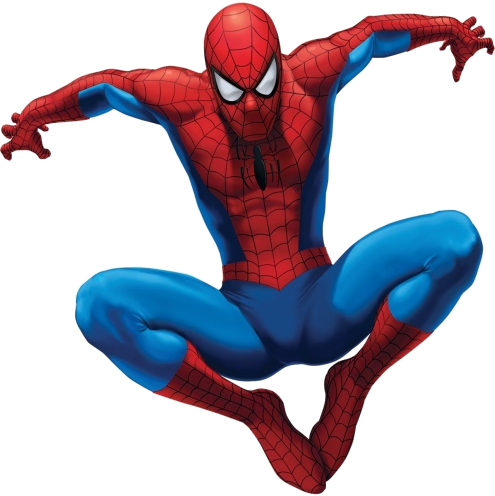
\includegraphics[height=2.9cm]{les2-hero-1}};
\node[anchor=north] (hero2) at (0.8,2.05)
{
\includegraphics[height=4cm]{les2-hero-2}};
\node[anchor=north] (hero3) at (1.3,1.575)
{
\includegraphics[height=3.1cm]{les2-hero-3}};
\node[anchor=north] (hero4) at (1.8,2.1)
{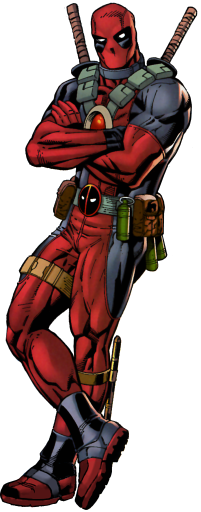
\includegraphics[height=4.1cm]{les2-hero-4}};
\node[anchor=north] (hero5) at (2.3,1.95)
{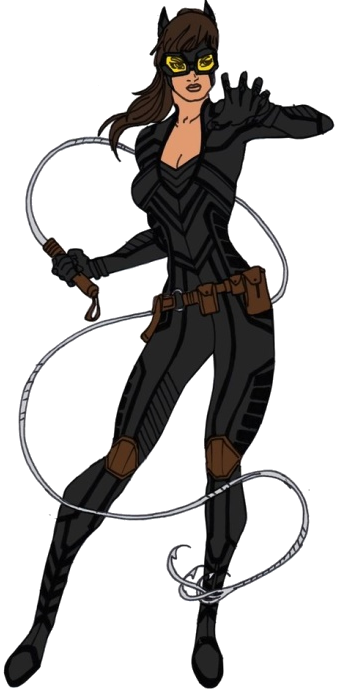
\includegraphics[height=3.8cm]{les2-hero-5}};

\node (size1) at (0.3, 1.5) {\scriptsize 141 cm};
\node (size2) at (0.8, 2.1) {\scriptsize 198 cm};
\node (size3) at (1.3, 1.51) {\scriptsize 143 cm};
\node (size4) at (1.8, 2.15) {\scriptsize 201 cm};
\node (size5) at (2.3, 1.95) {\scriptsize 184 cm};
\end{tikzpicture}

  \caption{Superhero sizes, in cm.}
  \label{fig:heroes-size}
\end{figure}

\subsection{Arithmetic mean}
\label{ssec:arithmetic-mean}

\begin{definition}[Arithmetic mean]
    \label{def:mean}
    
    The \emph{arithmetic mean}\index{mean!arithmetic} or \emph{average} (notation $\overline{x}$, x-bar) of a set of values is the sum of all values divided by the number of values.
    \begin{equation}
    \overline{x} = \frac{1}{n} \times \sum_{i=1}^{n} x_{i}
    \label{eq:Mean}
    \end{equation}
    
    With:
    \begin{itemize}
        \item $x_{i}$ the different values of a set (in the example of Figure~\ref{fig:heroes-size}: 141, 198, 143, etc.)
        \item $n$ the number of values (in the example is $n = 5$).
    \end{itemize}
\end{definition}

\begin{remark}[!!]
    Note that the symbol $\overline{x}$ specifically indicates the average of a \emph{sample}.
    The average of a \emph{population} is indicated by the Greek letter mu, $\mu $.
    
    See Appendix~\ref {app:notation} for an overview of the symbols and notations used in this syllabus.
\end{remark}

\begin{exercise}
    What is the average length of the superheroes in Figure~\ref{fig:heroes-size}?
\end{exercise}

\begin{exercise}
    The average of 15 numbers is 12. What number do we need to add to get an average of 13?
\end{exercise}

\begin{exercise}
    The arithmetic mean is sensitive to outliers, i.e. values far away from the mean. Extreme values can heavily influence the arithmetic mean.
    
    Assume that Kabout Wesley (10 cm) is added to the team of superheroes. What happens to the arithmetic mean?
\end{exercise}

\subsection{Variance and standard deviation}
\label{ssec:variance-and-standard-deviation}

The dispersion measure that is typically associated with the average is the standard deviation.
Before defining the standard deviation, we first provide the definition of the \emph{variance}.

\begin{definition}[Variance]
    The \emph{variance}\index{variance} (notation: $s^{2}$) of a sample is the mean squared difference between the values of the sample and the arithmetic mean.
    \begin{equation}
    s^{2} = \frac{1}{n-1} \times \sum_{i=1}^{n} \left( \overline{x} - x_i \right)^{2}
    \label{eq:variance}
    \end{equation}
\end{definition}

You may have noticed that in the formula the denominator is $n-1$ and not $n$, which you would expect. However, there is a variant of the formula with $n$ in the denominator. This latter one is called the population variance, indicated by $\sigma^2 $ (the Greek letter sigma).

The variance of a sample is used in practice as an estimate for the (unknown) population variance. The formula with $n-1$ in the denominator is a so-called \textit{pure estimator}, which means that in many repetitions the average of the estimates converges to the population variance. You can prove this mathematically, but this is beyond the scope of this course.

\begin{example}
    The variance of the length of our superheroes is calculated as follows:
    
    \begin{align*}
    s^{2} & =  \frac{(173,4 - 141)^{2} + (173,4 - 198 )^{2} + (173,4 - 143)^{2} + (173,4 - 201)^{2} + (173,4 - 184 )^{2}}{4} \\
    & =  \frac{(-32,4)^{2} + (24,6)^{2} + (-30,4)^{2} + (27,6)^{2} + (10,6)^{2}}{4}                                    \\
    & = \frac{1049,76 + 605,16 + 924,16 + 761,76 + 112,36}{4}                                                          \\
    & = \frac{3453,2}{4} = 863,3
    \end{align*}
\end{example}

When calculating the variance of our sample, we divide by $n-1$ and not by $n$. Why? 
As the sum of the deviations $x_{i} - \overline {x} $ always returns 0 (see below in Equation~\ref{eq:sumAvg}), the last deviation can be derived from the first $n-1$ deviations. Therefore we do not calculate the average of $n$ numbers without relationship. Only $n-1$ of the squared deviations can move freely, so we calculate the average by dividing the total by $n-1$. The number $n-1$, the number of logically independent values, is also called the \index{degrees of freedom} \emph{degrees of freedom}.

\begin{equation}
\sum_{i}^{n}(x_{i} - \overline{x}) = \sum_{i}^{n}x_{i} - \sum_{i}^{n}\overline{x} = \sum_{i}^{n}x_{i} - n \left(\frac{1}{n}\sum_{i}^{n} x_{i}\right)
\label{eq:sumAvg}
\end{equation}

\begin{definition}[Standard deviation]
    The \emph{standard deviation}\index{standard deviation} is the square root of the variance.
    \begin{equation}
    s = \sqrt{s^{2}} = \sqrt{\frac{1}{n-1} \sum_{i=1}^{n} \left(\overline{x} - x_i \right)^{2}}
    \label{eq:stdev}
    \end{equation}
\end{definition}

\begin{remark}[!!]
    In this definition we also explicitly defined the variance and standard deviation of a \emph{sample}. The standard deviation of a \emph{population} is indicated by the Greek letter sigma, $\sigma$.
\end{remark}

The standard deviation provides insight into what is normal and abnormal: 
A small standard deviation indicates that the values are close to the central tendency (arithmetic mean, $\overline{x}$),while  a large standard deviation indicates that the values are dispersed over a larger range of values. In some cases, a small standard deviation is desired, in other cases, it may not be that important, as illustrated below.

\begin{example}
  In the manufacturing process of screw drivers, the size of the head is important for its functioning. When the heads of a batch of 1000 screw drivers is measured, their sizes should be very similar, so a very small standard deviation is an indication of good quality.    
\end{example}

\begin{example}
  Super heroes are a very diverse group. Some are very rich (e.g.~Batman, Iron Man), some are middle class (e.g.~Spiderman), others are quite poor (e.g.~Arsenal). The dispersion of their income would be very large, but that isn't necessarily a bad thing.
\end{example}

An interesting property of the standard deviation is that it is expressed in the same unit as the measured data. In the example (size of superheroes), the standard deviation is 29,38 cm. 

Just like the arithmetic mean, the variance and standard deviation are sensitive to outliers. The variance is even more sensitive than the mean, because of the squared differences.

\subsection{Median}
\label{ssec:median}

The median is also a measure for central tendency. Compared to the arithmetic mean, the median is much less sensitive to outliers.

\begin{definition}[Median]
    The \emph{median}\index{median} is the value separating the higher half of a data set from the lower half. When you sort the values from low to high, the median will be the value in the middle. If the set has an even number of values, the median is the average of the two values in the middle. 
\end{definition}

\begin{exercise}
    What is de median of the sizes of our superheroes?
\end{exercise}

\begin{exercise}
    What would be the median if Kabouter Wesley (10 cm) is added to the group? 
    Is the impact bigger or smaller compared to the arithmetic mean?
\end{exercise}

\subsection{Range}
\label{ssec:range}

\begin{definition}[Range]
    The \emph{range}\index{range} of a dataset is the absolute value of the difference between the highest and the lowest value.
    \begin{equation}
    | max_i(x_i) - min_i(x_i) |
    \end{equation}    
\end{definition}

The range of a variable is often not interesting as a measure for dispersion, because it is very sensitive to outliers.


\subsection{Quartiles and Interquartile Range}
\label{ssec:quartiles}

The interquartile range is a better measure for dispersion, as it is less sensitive to outliers.
To understand the interquartile range, we first have to introduce the concept of \emph{quartiles}.

\begin{definition}[Quartiles]
    The \emph{quartiles}\index{quartiles} of a sorted set of numbers are the three values that divide the set into 4 equally large subsets.
    
    \begin{itemize}
        \item the first/lower quartile ($Q_{1}$) is the value that separates the lowest quarter of values from the rest
        \item the second quartile ($Q_{2}$) is the value that separates the lowest half of values from the highest half.
        \item the third/higher quartile ($Q_{3}$) is the value that separates the highest quarter of values from the rest
    \end{itemize}
\end{definition}

To determine the values of the quartiles in a sorted set, you can follow this approach~\autocite{Moore2002}:

If $n$ is an odd number, then:
\begin{itemize}
    \item $Q_{1}$ is the $\frac{n+1}{4}$th value;
    \item $Q_{3}$ is the $\frac{3n+3}{4}$th value.
\end{itemize}

If $n$ is an even number:
\begin{itemize}
    \item $Q_{1}$ is the $\frac{n+2}{4}$th value;
    \item $Q_{3}$ is the $\frac{3n+2}{4}$th value.
\end{itemize}

\begin{exercise}
    The second quartile, $Q_2$ corresponds to which other metric introduced in this chapter?
\end{exercise}

\begin{definition}[Interquartile range]
    The \emph{interquartile range}\index{range!interquartile} ($IQR$) is the difference between the higher and lower quartile.
    \begin{equation}
    IQR = Q_3 - Q_1
    \end{equation}
\end{definition}

The concept of quartiles can be generalized to percentages. The $P$-th \emph{percentile} of a list of ordered values is the smallest value in the list so that $P$ percent of the data is less than or equal to that value.


\section{Visualization of a Single Variable}

Even when visualizing one variable, the most suitable chart type depends on the measurement level.
Table~\ref{tab:charttypes-1-variable} provides an overview.
.

\begin{table}
    \centering
    \begin{tabular}{ll}
        \toprule
        \textbf{Measurement Level} & \textbf{Chart Type}   \\
        \midrule
        Qualitative         & Bar chart of frequencies     \\
        \midrule
        Quantitative        & Box plot, histogram, density \\
        \bottomrule
    \end{tabular}
    \caption{Suitable chart types per measurement level for visualizing a single variable.}
    \label{tab:charttypes-1-variable}
\end{table}

\subsection{Bar Chart}

When visualizing a qualitative variable, a frequency table is first calculated for all occurring values.

\begin{definition}[Frequency table]
    A \emph{frequency table}\index{frequency table} is a table that summerizes how often each value occurs in the data set.
    Frequency tables are usually vertically oriented.
\end{definition}

To draw a \index{bar chart}\emph{bar chart} (cfr. Figure~\ref{fig:barchart}), the different values are listed below the X-axis and for each value a bar is drawn whose height is determined by the number of times the corresponding value occurs.

\begin{figure}
    \centering
    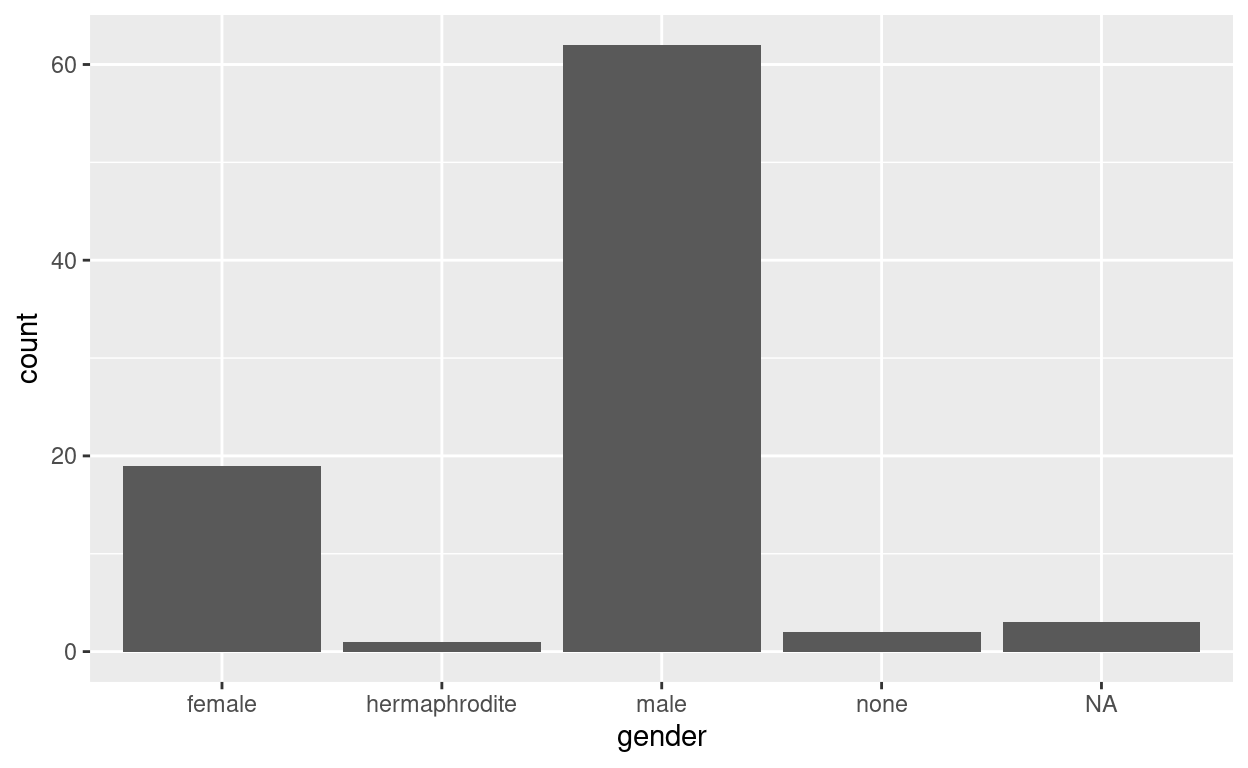
\includegraphics[width=.7\textwidth]{barchart}
    \caption[Example of a bar chart]{\textbf{Example of a bar chart.} The labels on the x-axis indicate the possible values of the visualized qualitative variable. The height of each bar indicates the frequency of each value within the sample.}
    \label{fig:barchart}
\end{figure}

\subsection{Box Plot}

A \index{box plot}\emph{box plot} is a chart that shows the dispersion of a set of values (cfr. Figure~\ref{fig:boxplot}). It is formed by a rectangle with sides at the quartiles ($Q_1$ and $Q_3$). Inside the rectangle, the median is drawn as well. The whiskers attached to the upper and lower sides of the rectangle cover the rest of the observations, except for outliers and extremes.

\begin{itemize}
    \item An \emph{outlier}\index{outlier} is a value that is more than 1.5 times the IQR below the lower quartile or above the higher quartile. It is indicated by a circle.
    \item An \emph{extreme value}\index{extreme} is a value that is more than 3 times the IQR below the lower quartile or above the higher quartile. It is indicated by a star.
\end{itemize}

A box plot is oriented horizontally or vertically, based on what is clearest.

\begin{figure}
    \centering
    % Source: http://mirrors.ibiblio.org/CTAN/graphics/pgf/contrib/pgfplots/doc/pgfplots.pdf
    % p.430
    \begin{tikzpicture}
    \begin{axis}[x=3cm,xticklabels={},xmax=2.3]
    \addplot+[
    boxplot prepared={
        draw direction=y,
        lower whisker=5,
        lower quartile=7,
        median=8.5,
        upper quartile=9.5,
        upper whisker=10,
    },
    ]
    table[row sep=\\,y index=0] {
        data\\ 1\\ 3\\
    }
    [right,color=hgorange]
    node at (boxplot box cs: 1,.6) {outlier}
    node at (boxplot box cs: \boxplotvalue{lower quartile},1) {$Q_1$}
    node at (boxplot box cs: \boxplotvalue{median},1)         {$Q_2$, median}
    node at (boxplot box cs: \boxplotvalue{upper quartile},1) {$Q_3$}
    node at (boxplot box cs: \boxplotvalue{upper whisker},1)  {max}
    ;
    \end{axis}
    \end{tikzpicture}
    \caption[Example of a box plot]{\textbf{Example of a box plot.} The blue rectangle indicates the interval in which half of the measured values are located. The limits are the first quartile at the bottom ($Q_1$) and the third quartile at the top ($Q_3$). The line in the middle of the rectangle is the median (or the second quartile, $Q_2$). The other blue horizontal lines in theory indicate the smallest and largest values. In this case, however, there are some observations that are very far from the median. These are called outliers and are plotted separately as individual points.}
    \label{fig:boxplot}
\end{figure}

\subsection{Histogram}

A \index{histogram}\emph{histogram} (cfr. Figure~\ref{fig:histogram}) is a kind of bar chart, but adjusted for quantitative variables.
The range of the variable is subdivided into a number of, typically equal, intervals or classes. For each class, the number of observations is counted and the height of the bars is determined based on this number.

\begin{figure}
    \centering
    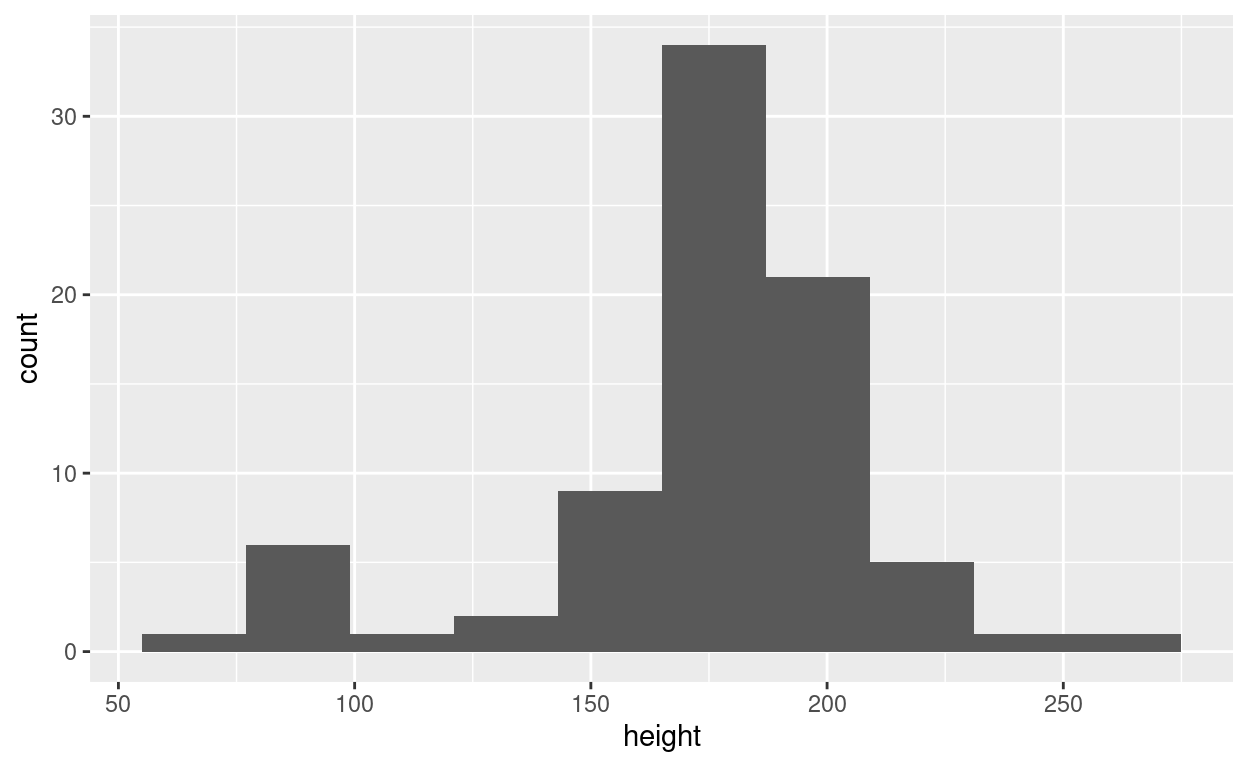
\includegraphics[width=.7\textwidth]{histogram}
    \caption[Example of a histogram]{\textbf{Example of a histogram.} The X-axis is subdivided into a number of equally large intervals. The height of each bar is based on the number of observations within each interval.}
    \label{fig:histogram}
\end{figure}

\subsection{Density Graph}

The clarity of a histogram largely depends on the choice of intervals. If these are chosen too large, you will lose precision, and if they are too small, different intervals will not contain any observations. As an alternative to a histogram, you can also plot a \index{density graph}\emph{density graph} (cfr. Figure~\ref{fig:dichtheidsgrafiek}). In this graph, the X-axis is not subdivided into classes. Instead, a continuous curve is drawn, and the height of this curve corresponds to the amount of observations ``in the neighborhood''. A density graph typically shows even better how the observations are spread.

\begin{figure}
    \centering
    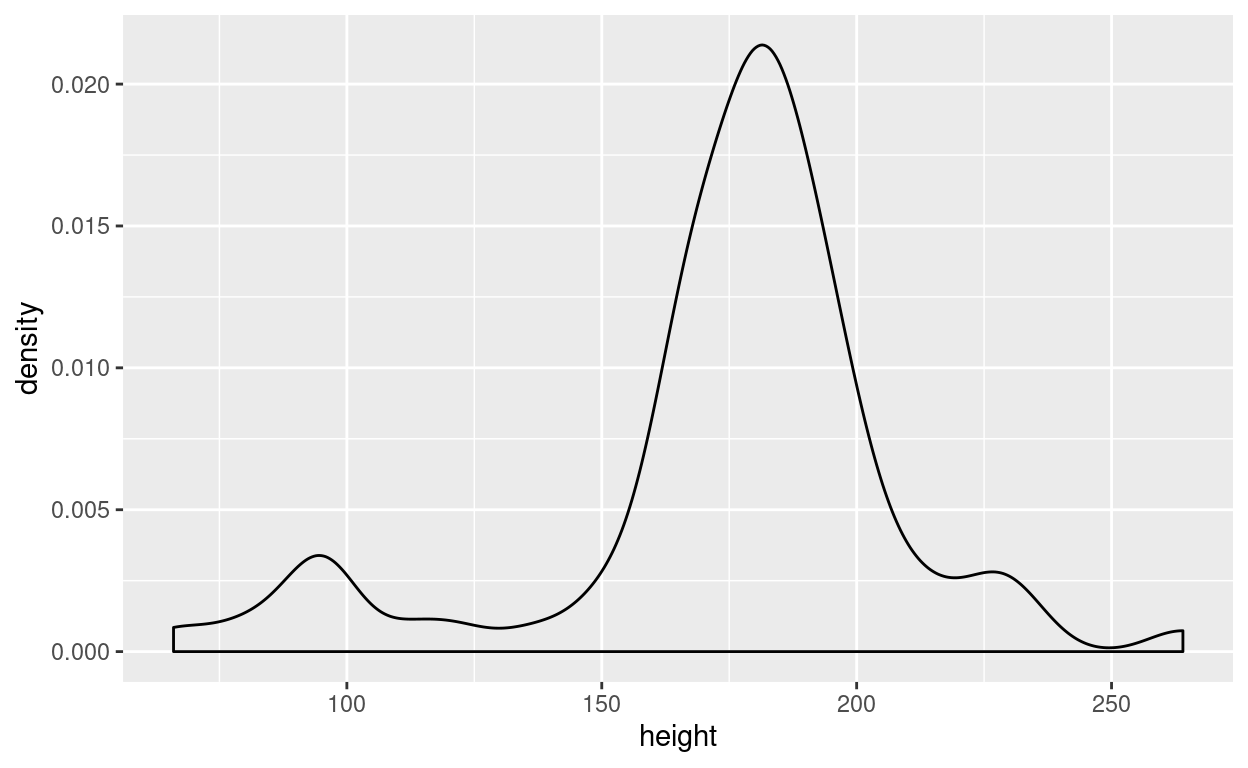
\includegraphics[width=.7\textwidth]{dichtheidsgrafiek}
    \caption[Example of a density graph]{\textbf{Example of a density graph.} The graph shows the same data as the histogram in Figure~\ref{fig:histogram}.}
    \label{fig:dichtheidsgrafiek}
\end{figure}

\section{Exercises}
\label{sec:exercises-univariate-analysis}

\subsection{Central Tendency and Dispersion}

\begin{exercise}
  \label{ex:mean-stdev-freq}
  The formulas for the sample mean $\overline{x}$, variance $s^2$ and standard deviation $s$ can be found in Section~\ref{ssec:arithmetic-mean} and~\ref{ssec:variance-and-standard-deviation} respectively.
  How should these formulas  be adapted to be used with a frequency table? Apply these formulas to the data provided in Table~\ref{tab:pinfreq}.
\end{exercise}

\begin{table}
  \centering
  \begin{tabular}{@{}ll@{}}
    \toprule
    Pins $x$ & Frequence $f_{x}$ \\ 
    \midrule
        0      &         2          \\
        1      &         1          \\
        2      &         2          \\
        3      &         0          \\
        4      &         2          \\
        5      &         4          \\
        6      &         9          \\
        7      &         11         \\
        8      &         13         \\
        9      &         8          \\
        10     &         8          \\
    \bottomrule
  \end{tabular}
  \caption{Frequency table for the number of pins knocked down in a game of bowling.}
  \label{tab:pinfreq}
\end{table}

\begin{exercise}
  \label{ex:variance-formula}
  Why does variance (see Equation~\ref{eq:variance}) use the square of the differences? Why not the actual values themselves (i.e. $(\overline{x} - x_i)$) or the absolute value of the difference (i.e. $\left|\overline{x} - x_i\right|$)?
  
  \begin{align}
  s^{2}_{1} &= \frac{1}{n-1} \sum_{i=1}^{n} (\overline{x} - x) \\
  s^{2}_{2} &= \frac{1}{n-1} \sum_{i=1}^{n} \left| \overline{x} - x\right| \\
  s^{2}_{3} &= \frac{1}{n-1} \sum_{i=1}^{n} (\overline{x} - x)^{2}
  \end{align}
  
  Try out each variant of the equation for both datasets $X = \left\{4,4,-4,-4\right\}$ and $Y = \left\{7,1,-6,-2\right\}$.
\end{exercise}

\begin{exercise}
  Find out what the \emph{coefficient of variation} (CV) means. How is it defined? What is the major difference with the standard deviation?
\end{exercise}

\begin{exercise}
  \label{ex:ais}
  Import the file \texttt{ais.csv} in R (this file is available in the Github repository of this course, inside the folder \texttt{exercises/datasets}). 
  A description of this data frame can be found in the same folder, file \texttt{ais.html}.

  You can import this file in R using the following code:
  \begin{lstlisting}
  ais <- read.csv("ais.csv", sep = ",")
  attach(ais)
  \end{lstlisting}

  Consider the following subsets of this data frame, and calculate for each subset the appropriate measures for central tendency and dispersion for the variables \texttt{sex} and \texttt{ht}.

  \begin{enumerate}
      \item the rowers;
      \item the rowers, the netballers and the tennis players combined;
      \item the female basketball players and rowers.
  \end{enumerate}
\end{exercise}

\begin{exercise}
  \label{ex:mean-range-R}
  Use the functions \texttt{mean} and \texttt{range} in R to determine the mean and range of:
  \begin{itemize}
      \item the numbers 1, 2, \dots, 21.
      \item 50 random values, generated from a normal distribution with mean 0 and variance 1 (function \texttt{rnorm}).
      \item the columns \texttt{height} and \texttt{weight} of the data frame \texttt{women} (built-in in R).
  \end{itemize}
\end{exercise}


In previous exercises we described the different measures for central tendency and dispersion.
As you might have notices, these metrics are also used in the research of~\textcite{Akin2016}.
In the next exercies, we will try to reproduce the results.

For this, we need the file \texttt{android\_persistence\_cpu.csv}.
This file can also be found inside the folder \texttt{exercises/datasets} on GitHub.


\begin{exercise}
  \label{oef:casus-akin2016-1var}
  Open this file in a spreadsheet application and study the structure of the data. 
  Can you identify the variables and their measurement level?
\end{exercise}

We will be using the \texttt{R} programming language for statistical computing with RStudio. 

\begin{lstlisting}[breaklines=true]
  android_cpu <- read.csv("android_persistence_cpu.csv", sep=";", dec=".")
  attach(android_cpu)
\end{lstlisting}

You can use the above code to import the file in R. 
After importing the file, try to calculate the average execution time, the standard deviation, the different quantiles, etc.
Use the commands \texttt{mean}, \texttt {median}, \texttt {quantile}, \texttt {min}, \texttt{max}, \texttt{var}, \texttt{sd}. 
You can also use the \texttt{summary} command to get a nice overviw.

Tips:

\begin{itemize}
  \item A column/variable of a data table is referred to as: \verb|Table$Column|. When you have \verb|attach|ed the table, you can use the \verb|Column| name directly.
  \item You can group values according to a qualitative value with \verb|Variable ~ Categories|.
\end{itemize}


\begin{exercise}
  Is it possible to draw conclusions from these results? If so, what are they? If not, why not?
\end{exercise}

\subsection{Charts in R}
\subsubsection{Histogram}

A histogram is a plot that shows the frequencies of observations between specific ranges.

\begin{lstlisting}[breaklines=true]
  hist(android_cpu$Time, main="Distribution of execution time", xlab="Execution time (ms)")
  hist(android_cpu$Time, main="Distribution of execution time", xlab="Execution time (ms)", breaks=2)
\end{lstlisting}

\begin{exercise}
  Can you draw useful conclusions from this graph\footnote{You can find general info about generating plots in R here:  \url{https://www.datacamp.com/community/tutorials/15-questions-about-r-plots\#gs.RK_ORsI}.}? 
  What happens if you increase the number of \texttt{breaks}?
\end{exercise}

\subsubsection{Boxplot}

A boxplot shows the median, quartiles, and extremes in a dataset. 
It provides a good overview of the distribution of the data.

\begin{lstlisting}[breaklines=true]
  boxplot(android_cpu$Time)
  boxplot(android_cpu$Time, main='Distribution of execution time', ylab="Execution time (ms)")
\end{lstlisting} 

\begin{exercise}
  By default, boxplots are drawn vertically. Use the help function in RStudio to find out how to draw it horizontally.
\end{exercise}

In the previous exercises, when we tried to analyse the dataset as a whole, we noticed that this is pretty much useless, since the data set is divided into several categories. 
Let's create separate boxplots for each category.

\begin{lstlisting}[breaklines=true]
  boxplot(android_cpu$Time ~ android_cpu$DataSize, main="Distribution of CPU time over the data sizes", ylab="Time in ms");
\end{lstlisting}

\begin{exercise}
	\label{ex:boxplot}
  Interpret the results from this plot. Do these make more sense?
\end{exercise}

We can do the same for the different persistence types.

\begin{exercise}
  Do the same as in \ref{ex:boxplot}, but group by \verb|PersistenceType| and interpret the results. Do these make sense?
\end{exercise}

Finally, let's see how the data is distributed over \emph{both} categories.

\begin{lstlisting}[breaklines=true]
  boxplot(android_cpu$Time ~ android_cpu$PersistenceType * android_cpu$DataSize, main="Distribution of CPU time over data sizes for the different persistent types", ylab="Time in ms");
\end{lstlisting}

By looking at the data over the different categories, we get a clearer view on the data, but the graph is a bit overcrowded now.

There are several ways of selecting data that meets specific criteria, a.o.~the functions \verb|which| and \verb|subset|.

\begin{lstlisting}[breaklines=true]
  greenDOA <- android_cpu[which(android_cpu$PersistenceType=='GreenDAO'),];
  boxplot(greenDOA$Time ~ greenDOA$DataSize);
\end{lstlisting}

\begin{exercise}
  Wat can you conclude from this plot?
\end{exercise}

\begin{exercise}
  Find out which box plots are meaningful for this data and whether your results match those of~\textcite{Akin2016}. What are your conclusions?
\end{exercise}

\begin{exercise}[Retrieval practice]
  Use the procedure for retrieval practice from exercise~\ref{ex:retrieval-practice-meetniveaus} 
  to study the \emph{techqniques for analysis and visualization of a single variable}.
  
  Provide for each measurement level:
  
  \begin{itemize}
    \item The appropriate measurements for central tendency and dispersion (name + definitions and formulas)
    \item The appropriate graph types
  \end{itemize}
\end{exercise}




%Exercise~\ref{ex:q2}: the median

%Exercise~\ref{ex:variance-formula}:

%\begin{itemize}
  %\item When using the values themselves, negative and positive values would cancel out each other, resulting in a variance of 0 in set $X$.
  %\item When using the absolute value, both data sets would have the same variance, although the dispersion of set $Y$ is clearly larger.
%  \item When squaring the differences, these problems do not occur.
%\end{itemize}



% Answers
\subsection{Solutions to selected exercises}

\paragraph{Exercise \ref{ex:mean-stdev-freq}}

\begin{itemize}
  \item $\overline{x} = 7$
  \item $s^2 \approx 5.830508$
  \item $s \approx 2.414645$
\end{itemize}

\paragraph{Exercise \ref{ex:variance-formula}}
Table~\ref{tab:opl-variance-ht} provides an overview of the adjusted sample variance for both datasets.

\begin{table}
  \centering
  \begin{tabular}{@{}l|rrr@{}}
    \toprule
      & \textbf{$s^{2}_{1}$} & \textbf{$s^{2}_{2}$} & \textbf{$s^{2}_{3}$} \\
    \midrule                
      \textbf{$ X $} & 0           & 5.333333    & 21.33333    \\ 
      \textbf{$ Y $} & 0           & 5.333333    & 30          \\           
    \bottomrule
  \end{tabular}
  \caption{Results of the adjusted sample variance for both datasets, for the different formulas of exercise~\ref{ex:variance-formula}.}
  \label{tab:opl-variance-ht}
\end{table}

\paragraph{Exercise \ref{ex:ais}}

Table~\ref{tab:opl-ais-ht} provides an overview of the most important measurements for central tendency and dispersion for the variable \texttt{ht} (height/length) for the requested groups.

\begin{table}
  \centering
  \begin{tabular}{@{}l|r|rrrr|rr@{}}
    \toprule
    & \textbf{(1)} & \multicolumn{4}{c}{\textbf{(2)}}                                                 & \multicolumn{2}{c}{\textbf{(3)}} \\ 
    & \textbf{Row} & \textbf{Total}    & \textbf{Row} & \textbf{Netball} & \textbf{Tennis} & \textbf{B\_ball}  & \textbf{Row} \\ \midrule
    \textbf{mean}       & 182.376      & 179.066                      & 182.376      & 176.087          & 174.164         & 182.269           & 178.859      \\
    \textbf{stdev}      & 7.798        & 7.936                        & 7.798        & 4.124            & 9.858           & 8.621             & 5.970        \\
    \textbf{min}        & 156.000      & 156.000                      & 156.000      & 168.600          & 157.900         & 169.100           & 156.000      \\
    \textbf{Q1}         & 179.300      & 174.200                      & 179.300      & 173.450          & 167.300         & 174.000           & 177.600      \\
    \textbf{median}     & 181.800      & 179.500                      & 181.800      & 176.000          & 175.000         & 184.600           & 179.650      \\
    \textbf{Q3}         & 186.300      & 183.400                      & 186.300      & 179.150          & 180.750         & 188.700           & 181.200      \\
    \textbf{max}        & 198.000      & 198.000                      & 198.000      & 183.300          & 190.800         & 195.900           & 186.300      \\
    \textbf{IQR}        & 7.000        & 9.150                        & 7.000        & 5.700            & 13.450          & 14.700            & 3.600        \\ \bottomrule
  \end{tabular}
  \caption{Overview results Exercise~\ref{ex:ais} for the variable \texttt{ht} (height/length).}
  \label{tab:opl-ais-ht}
\end{table}

In part 1 and 2 we take the variable \texttt{sex} as an example, cfr. Table~\ref{tab:opl-ais-sex} for an overview.
We cannot say much about qualitative variables, so we provide a frequency table from which we can derive the mode.

In part 3 only women are selected, and Table~ \ref{tab:opl-ais-sport} illustrates the frequencies of the variable \texttt{sport}.

\begin{table}
  \centering
  \begin{tabular}{@{}l|r|rrrr}
  	\toprule
  	               & \textbf{(1)} &                    \multicolumn{4}{c}{\textbf{(2)}}                     \\
  	               & \textbf{Row} & \textbf{Whole group}& \textbf{Row} & \textbf{Netball} & \textbf{Tennis} \\ \midrule
  	\textbf{f}     &           22 &                  52 &           22 &               23 &               7 \\
  	\textbf{m}     &           15 &                  19 &           15 &                0 &               4 \\
  	\textbf{mode}  &            f &                   f &            f &                f &               f \\ \bottomrule
  \end{tabular}
  \caption{Overview results Exercise~\ref{ex:ais} (1) and (2) for the variable \texttt{sex}. This table provides the different frequencies, as well as the mode.}
  \label{tab:opl-ais-sex}
\end{table}

\begin{table}
  \centering
  \begin{tabular}{@{}l|l}
  	\toprule
  	                 & Frequency   \\ \midrule
  	\textbf{B\_ball} & 13          \\
  	\textbf{Row}     & 22          \\
  	\textbf{modus}   & Row         \\ \bottomrule
  \end{tabular}
  \caption{Overview results Exercise~\ref{ex:ais} (3) for the variable \texttt{sport}.}
  \label{tab:opl-ais-sport}
\end{table}


\paragraph{Exercise \ref{ex:mean-range-R}}
Table~\ref{tab:opl-mean-range-R} provides an overview of the mean and range for exercise~\ref{ex:mean-range-R}.

\begin{table}
  \centering
  \begin{tabular}{@{}l|r|rl@{}}
    \toprule
      & \textbf{Mean} & \multicolumn{2}{c}{\textbf{Range}} \\
    \midrule                
                  \textbf{$1,2,...,21$} & 11       & 1    & 21    \\ 
        \textbf{\texttt{women\$height}} & 65       & 58   & 72    \\
        \textbf{\texttt{women\$weight}} & 136.7333 & 115  & 164   \\
    \bottomrule
  \end{tabular}
  \caption{Mean and range for the datasets of Exercise~\ref{ex:mean-range-R}.}
  \label{tab:opl-mean-range-R}
\end{table}
\chapter{The Central Limit Theorem}
\label{ch:central-limit-theorem}

In this chapter the central limit theorem in introduced (cfr. Section~\ref{sec:central-limit-theorem}). This theorem is a key concept in probability theory, because multiple statistical testing procedures (cfr. Chapter~\ref{ch:testing-procedures}) are based on this. The central limit theorem allows you to generalize measurements obtained from a sample to the full population under certain conditions.

We also discuss the concept of point estimators and confidence intervals. A point estimator is a number that is calculated from the sample, which can be used to estimate a property of the population. For example, the mean/average of a sample $\overline{x}$ is a point estimator for the mean/average of the population $\mu$. A confidence interval is used to propose a range of plausible values for an unknown parameter together with an associated confidence level. For example, a 95\% confidence interval for the mean of a population is an interval derived from the sample, of which we can say that - under clear conditions - the population mean has a 95\% chance to be in the proposed range.

But before introducing these concepts, we first start with a short rehearsal of general concepts of the probability theory (cfr. Section~\ref{sec:probability-distribution-sample}) and discuss the normal distribution (cfr Section~\ref{sec:normal-distribution}).

\section{Learning Goals}
\label{sec:central-limit-theorem-learning-goals}

By the end of this chapter you must be able to:

\begin{itemize}
  \item Explain and apply the following concepts:
  \begin{itemize}
    \item Sample Space (universum), event, probability space, probability, discrete/continuous probability distribution
    \item Point Estimator, confidence interval
    \item Degrees of freedom
  \end{itemize}
  \item Sketch the probability distribution of the normal distribution for a given mean and standard deviation (Gaussian curve) and indicate the mean and standard deviation on this graph;
  \item Calculate the $z$ score of a value in a normally distributed random variable;
  \item Calculate the left- ($P(X<x)$) and right tail-probability ($P(X>x)$) or combinations of both (eg. $P(x<X<y)$) for a value in a normally distributed calculate stochastic variable, using the symmetry rule and the 100\% rule where necessary;
  \item Determine to what extent a given stochastic variable is normally distributed based on the probability density curve, QQ plot, skewness or kurtosis;
  \item Formulate the central limit theorem (and in particular know the probability distribution of the sample mean) and explain its importance for statistical analysis.
  \item Calculate a confidence interval for the population mean of a sample with a given confidence level in the following cases:
  \begin{itemize}
    \item a large sample with known population variance
    \item a small sample with unknown population variance
    \item a sampling fraction
  \end{itemize}
\end{itemize}

\section{Probability Distribution of a Sample}
\label{sec:probability-distribution-sample}

\subsection{Stochastic Experiment}
A random (or stochastic) experiment requires the following elements:

\begin{definition}[Sample Space or Universum]\
   The sample space or universum of an experiment
   is the collection of all possible outcomes of this experiment and
   is denoted by $\Omega$.
   \end{definition}

   \textbf{Remarks}
   \begin{itemize}
   \item The sample space needs to be \emph{complete} or \emph{collectively exhaustive}\/: 
   Every possible outcome of an experiment should be an element of $\Omega$.
   \item Additionally, it needs to be \emph{mutually exclusive}\/:
   Every outcome of an experiment should correspond with \emph{exactly one} element of $\Omega$.
   \item In summary: after executing an experiment it should be unambiguous 
   to indicate what element of $\Omega$ has occured.
   \end{itemize}
   
   \begin{definition}[Event]
    An \emph{event}\index{event} is a subset of the sample space. A singular or elementary event is a singleton. A composite event has a cardinality greater than 1.
\end{definition}

When $A$ and $B$ are events, the following events can be formed:
\begin{itemize}
    \item $A$ \textbf{or} $B$, noted as $A \cup B$;
    \item $A$ \textbf{and} $B$, noted as $A \cap B$;
    \item \textbf{not} $A$, noted as $\overline{A}$.
\end{itemize}

Events that don't have common outcomes are called \emph{disjoint}\index{event!disjoint}.
Consequently, disjoint events can never occur simultaneously. 
When events $A$ and $B$ are disjoint, then $A \cap B = \emptyset$. 

\textbf{Remarks}
\begin{itemize}
   \item It can be proven by induction that the union of $n$ events $A_1$ up to $A_n$ is also an event.
   \item The same goes for the intersection between events.
   \item For some application, countable infinite unions or intersections are also considered.
\end{itemize}
   
\begin{definition}[Probability space] 
    The probability of an event $A$ is noted as $P(A)$. Probabilities of events should meet the following requirements:

   \begin{enumerate}
   \item Probabilities of events are positive: $\forall A \subset \Omega: P(A) \geq 0$
   \item The total probability of all elements in $\Omega$ is 1: $P(\Omega) = 1.$
   \item If $A$ and $B$ are \emph{disjoint} events, then:
    \[P(A\cup B) = P(A) + P(B). \]
    This is called the Rule of Sum.
   \end{enumerate}

   When the probability function $P$ meets these requirements (axioms), 
   then the triple $(\Omega, \mathcal{P}(\Omega), P)$ is a \emph{probability space}\index{probability space} 
   (with $\mathcal{P}(\Omega)$ the \emph{power set} of $\Omega$, i.e.~the set of all its subsets).
\end{definition}
   
\begin{example}
\label{ex:dice}
    Consider a sample space $\Omega =  \left\{ 1,2,3,4,5,6 \right\} $ and a probability function $P(\omega) = \frac{1}{|\Omega|}$. 
    This combination could represent a dice with 6 sides, and outcomes $1, \ldots, 6$, each having a probability $P(\omega) = \frac{1}{6}$.
\end{example}
   
In this part of the syllabus we will look at \textbf{statistical inference}: make statements about the population based on a drawn sample.

\subsection{Probability distribution}
\label{ssec:probability-distribution}
   
\subsubsection{Discrete probability distribution}

If we continue the example of rolling a dice (cfr Example~\ref{ex:dice}), the probability of each outcome $\Omega = \{1,2,3,4,5,6\}$ can be summarized using a table or histogram (cfr. Figure~\ref{fig:probabilities-1-dice}). Some important notes:

\begin{enumerate}
    \item All probabilities are nonnegative.
    \item The probability of a specific outcome equals the area of the corresponding bar.
    \item The total area of all bars is 1.
\end{enumerate}

\begin{figure}
    \centering
    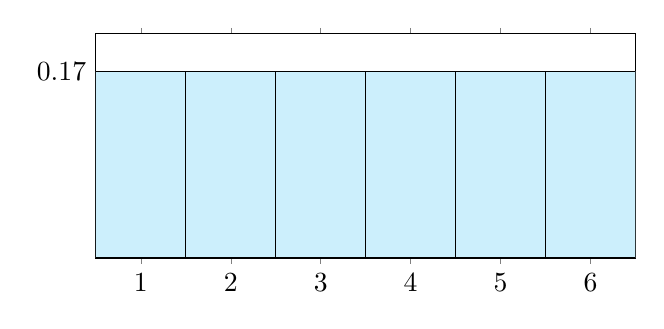
\begin{tikzpicture}
    \begin{axis}[ybar,ytick=data,ymin=0, ymax=.2, anchor=north, bar width=1, yscale=.5]
    \addplot[fill=cyan!20]
    coordinates {
        (1, 1/6)
        (2, 1/6)
        (3, 1/6)
        (4, 1/6)
        (5, 1/6)
        (6, 1/6)};
    \end{axis}
    \end{tikzpicture}
    \caption{Probability distribution when rolling a single dice.}
    \label{fig:probabilities-1-dice}
\end{figure}

When rolling \emph{two} dice, there are $6 \times 6 = 36$ possible outcomes, but some of them are equivalent. 
For example, $5$ and $2$, $2$ and $5$, $3$ and $4$, etc. all have a total outcome of $7$. 
There are two ways to roll a $3$. Consequently, $P(X=3) = \frac{2}{36}$. 
For $n = 1, \ldots, 7$, it holds that $P(X=n) = \frac{n-1}{36}$. 
Figure~\ref{fig:probabilities-2-dice} shows the corresponding histogram of the probability distribution.

\begin{figure}
    \centering
    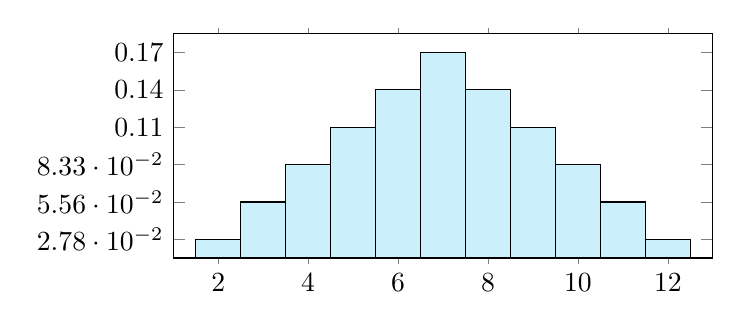
\begin{tikzpicture}
    \begin{axis}[ybar,ytick=data, anchor=north, bar width=1, yscale=.5]
    \addplot[fill=cyan!20]
    coordinates {
      (2, 1/36)
      (3, 2/36)
      (4, 3/36)
      (5, 4/36)
      (6, 5/36)
      (7, 6/36)
      (8, 5/36)
      (9, 4/36)
      (10, 3/36)
      (11, 2/36)
      (12, 1/36)
    };
    
    \end{axis}
    \end{tikzpicture}
    \caption{Probability distribution when rolling two dice.}
    \label{fig:probabilities-2-dice}
  \end{figure}

The histogram allows for the following calculations:
\begin{itemize}
  \item The probability of rolling a 10 or higher is the sum of the area of bars 10, 11, and 12.
  \item The probability of rolling a number between 2 and 7 (not included) is the sum of the area of bars 3, \ldots, 6.
  \item $\ldots$
  \item The total area is 1: the probability that 1 of all these outcomes occurs is 100\%.
\end{itemize}

\subsubsection{Continuous probability distribution}

Continuous probability distributions\index{probability distribution!continuous} are distributions where the sample space doesn't merely consist of a limited number of outcomes (nominal or ordinal level of measurement), but where outcomes can be any numeric value (interval and ratio level).
Take for example the weight of our superheroes: this is a continuous variable since a value can be not only a whole number like $70$ kg or $95$ kg, but also (approximately) $86,8735485653$ kg. In principle, any real value is possible, although in practice it's impossible to measure this exactly. This has an important consequence for the probability distribution. The distribution no longer consist of separate bars, but has become a continuous curve (cfr. Figure~\ref{fig:verdelingReactievermogen}). This implies that the probability of measuring exactly $70$ kg is effectively zero. However, when we say $70$ kg, we usually mean any value between $69.5$ and $70.5$ kg, or more precisely the interval $[69.5, 70.5[$. Likewise, $70,00000$ kg could refer to a value within the interval $[69.999995, 70.000005[$ kg.

The properties of probability distributions mentioned before still hold. The surface below the curve totals to 1. Also, the probability between two values is the surface below the curve, between the boundaries defined by these values. Remark that it's not actually important whether the limits are included or not, since their probabilities are negligable.

\section{The normal distribution}
\label{sec:normal-distribution}

\begin{figure}[t]
\centering
\begin{tikzpicture}
\begin{axis}[
  domain=0:10, samples=100,
  axis lines*=left, xlabel=$x$, ylabel=$y$,
  every axis y label/.style={at=(current axis.above origin),anchor=south},
  every axis x label/.style={at=(current axis.right of origin),anchor=west},
  height=5cm, width=12cm,
  xtick={5,3.5,6.5}, ytick=\empty,
  enlargelimits=false, clip=false, axis on top,
  grid = major
  ]
  \addplot [fill=cyan!20, draw=none, domain=0:9] {gauss(5,1.5)} \closedcycle;
  \draw [yshift=-0.6cm, latex-latex](axis cs:3.5,0) -- node [fill=white] {$\sigma$} (axis cs:5.0,0);
\end{axis}
\end{tikzpicture}
\caption{The probability of Superman's reaction speed. This curve illustrates the normal distribution with mean $\mu = 5$ ms and standard deviation $\sigma = 1.5 ms.$}
\label{fig:verdelingReactievermogen}
\end{figure}


Figure \ref{fig:verdelingReactievermogen} illustrates the probability distribution of Superman's reaction speed, variable $X$. The curve follows the normal distribution\index{distribution!normal} with a mean of 5 ms and a standard deviation of 1.5 ms. This is also notated as:
\[ X  \sim Nor(\mu = 5; \sigma = 1.5) \]

The equation of this function, the probability density, is sometimes referred to as the Gaussian bell curve, called after mathematician Carl Friedrich Gauss:
\begin{equation}
  f(x) = \frac{1}{\sigma \sqrt{2\pi}} e^{-\frac{1}{2} \frac{(x - \mu)^{2}}{\sigma^{2}}}
  \label{eq:normalFunction}
\end{equation}

De normal distribution has the following properties:
\begin{itemize}
  \item The probability density is bell-shaped;
  \item The probability density is symmetric around $\mu$;
  \item Because of this symmetry, the mean, median and mode are equal;
  \item The total area below the bell curve and above the $x$-axis is 1;
  \item The area between $\mu - \sigma$ en $\mu + \sigma$ (the so-called sigma area) contains approximately 68\% of the observations;
  \item The area between $\mu - 2 \sigma$ and $\mu + 2 \sigma$ contains about 95\% of all observations;
  \item The area between $\mu - 3 \sigma$ and $\mu + 3 \sigma$ contains about 99.7\% of all observations;
  \item The different areas are illustrated in Figure~\ref{fig:standard-normal-distribution}.
\end{itemize}

\subsection{The standard normal distribution}
\label{ssec:standard-normal-distribution}

If the distribution of stochastic variable $X$ is $X \sim N(\mu, \sigma)$, then the distribution of $Z = \frac{X - \mu}{\sigma}$ is $Z \sim N(0,1)$. This is called the standard normal distribution\index{distribution!standard normal}.

% Bron: http://johncanning.net/wp/?p=1202
\begin{center}
\begin{figure}
\centering
\begin{tikzpicture}
    \begin{axis}[
        no markers, domain=0:10, samples=100,
        axis lines*=left,height=6cm, width=10cm,
        xtick={-3, -2, -1, 0, 1, 2, 3}, ytick=\empty,
        enlargelimits=false, clip=false, axis on top,
        grid = major
    ]
    \addplot [smooth,fill=cyan!20, draw=none, domain=-3:3] {gauss(0,1)} \closedcycle;
    \addplot [smooth,fill=orange!20, draw=none, domain=-3:-2] {gauss(0,1)} \closedcycle;
    \addplot [smooth,fill=orange!20, draw=none, domain=2:3] {gauss(0,1)} \closedcycle;
    \addplot [smooth,fill=blue!20, draw=none, domain=-2:-1] {gauss(0,1)} \closedcycle;
    \addplot [smooth,fill=blue!20, draw=none, domain=1:2] {gauss(0,1)} \closedcycle;
    \addplot[<->] coordinates {(-1,0.4) (1,0.4)};
    \addplot[<->] coordinates {(-2,0.3) (2,0.3)};
    \addplot[<->] coordinates {(-3,0.2) (3,0.2)};
    \node[coordinate, pin={68.3\%}] at (axis cs: 0, 0.35){};
    \node[coordinate, pin={95.4\%}] at (axis cs: 0, 0.25){};
    \node[coordinate, pin={99.7\%}] at (axis cs: 0, 0.15){};
    \node[coordinate, pin={34.1\%}] at (axis cs: -0.5, 0){};
    \node[coordinate, pin={34.1\%}] at (axis cs: 0.5, 0){};
    \node[coordinate, pin={13.6\%}] at (axis cs: 1.5, 0){};
    \node[coordinate, pin={13.6\%}] at (axis cs: -1.5, 0){};
    \node[coordinate, pin={2.1\%}] at (axis cs: 2.5, 0){};
    \node[coordinate, pin={2.1\%}] at (axis cs: -2.5, 0){};
    \end{axis}
\end{tikzpicture}
\caption{The standard normal distribution with different ``zones'' indicating the percentage of observations within each zone.}
\label{fig:standard-normal-distribution}
\end{figure}
\end{center}

Often, it is useful to compare observations from different normal distributions. We can \emph{normalize} an observation by calculating the distance from the mean in terms of the standard deviation. This is called the $z$-score and is calculated as follows:

\begin{equation}
    z = \frac{x-\mu}{\sigma}
    \label{eq:zscore}
  \end{equation}

This score indicates how extreme an observation is, or in other words how many standard deviations it is located away from the mean. 
For a random value of $x$ we can use Equation~\ref{eq:zscore} to calculate the corresponding $z$-score.
The $z$-scores are so significant and often used that specific tables were composed containing the probabilities that an observation drawn from $Z$ is smaller than $z$, the so-called left tail probability\footnote{Similar tables containing the right tail probability exist as well}: $P(Z<z)$.

R also has functions for calculating with probabilities of normally distributed variables. These are summarized in Table~\ref{rab:norm-prob-r}.

\begin{table}
  \centering
  \begin{tabular}{ll}
  	\textbf{Function}     & \textbf{Description}                                           \\ \hline
  	\verb|pnorm(x, m, s)| & Left tail probability, $P(X<\mathtt{x})$                       \\
  	\verb|dnorm(x, m, s)| & Altitude of the Gaussian curve at point \texttt{x}             \\
  	\verb|qnorm(p, m, s)| & What boundary value contains \texttt{p}\% of the observations?\\
  	\verb|rnorm(n, m, s)| & Generate \texttt{n} normally distributed random numbers
  \end{tabular}

  \caption{Functions for calculating the probability in R for a normal distribution with mean \texttt{m} and standard deviation \texttt{s}. If the values for arguments \texttt{m} and \texttt{s} are omitted, the standard normal distribution is used.}
  \label{rab:norm-prob-r}
\end{table}

In order to calculate probabilities for any normal distribution, the following method can be used:

\begin{enumerate}
  \item Determine the stochastic variable with the associated normal distribution ($\mu$ and $\sigma$);
  \item Calculate the $z$-score for a given $x$-value;
  \item Reduce the requested probability to a left tail probability, using the probabilities of the normal distribution:
  \begin{itemize}
    \item $P(Z > z) = P(Z < -z)$ (symmetry rule);
    \item $P(Z > z) = 1 - P(Z < z)$ (100\% probability rule)
  \end{itemize}
\end{enumerate}

Plotting or sketching the requested probability is also very useful to gain insight into the calculation.

\begin{example}
What is the probability that Superman reacts in less than 4 ms?
\[ P(X < 4) = P(Z < -0,67) = 0,2514 \]
\end{example}

\begin{example}
What is the probability that he reacts in less than 7 ms?
\[ P(X < 7) = P(Z < 1,33) = 0,9082 \]
\end{example}

\begin{example}
What is the probability that he reacts in less than 3 ms?
\[ P(X<3) = P(Z < -1,33) = 0,0918 \]
\end{example}

\begin{example}
What is the probability that he reacts between 2 en 6.5 ms?
\[ P( 2 < X < 6,5) = P(X<6,5) - P(X<2) = P(Z<1) - P(Z<-2) = 0,8186 \]
\end{example}

\subsection{Testing for normality}
\label{ssec:testing-for-normality}

Because of the desirable properties of the normal distribution, it's often good to know whether a sample is actually drawn from a normal distribution. Several methods exist to test for normality:

\begin{enumerate}
  \item Plot a histogram for the data and look at the shape of the chart. If the observations are drawn from a normal distribution, the shape will approximate a bell curve.
  \item Calculate the intervals $\overline{x} \pm s$, $\overline{x} \pm 2s$, $\overline{x} \pm 3s$ and determine the percentage of observations in each interval. If the observations are normally distributed, these percentages should be around 68\%, 95\%, and 99,7\%, respectively.
  \item Draw a Q-Q plot\index{Q-Q plot} (normality plot, cfr. Definition~\ref{def:qq-plot}) for the observations. If they are normally distributed, the observations will be plotted approximately on a straight line.
  \item Calculate the \emph{kurtosis}\index{kurtosis}, a metric for the ``sharpness'' of the distribution's ``peak'':
    \begin{itemize}
      \item A normal distribution has a kurtosis of 3, or, alternatively, an \emph{excess kurtosis}\index{kurtosis!excess} of 0;
      \item A ``flat'' distribution has a negative excess kurtosis;
      \item A distribution with a sharp peak has a positive excess kurtosis.
      \item Note: when using the original definition of kurtosis, the normal distribution has a kurtosis of 3. We however use an alternative definition of kurtotis here, often referred to as the ``excess kurtosis'', which substracts 3 of the original value, resulting in a kurtosis of 0 for a normal distribution.
    \end{itemize}
  \item Calculate the \emph{skewness}\index{skewness}, a metric for the symmetry of the data:
    \begin{itemize}
      \item A symmetric distribution (including the normal distribution) has a skewness of 0;
      \item A distribution with a long left tail has a negative skewness;
      \item A distribution with a long right tail has a positive skewness;
      \item Rule of thumb: if the absolute value of the skewness $>1$, the distribution is not considered to be symmetrical.
    \end{itemize}
\end{enumerate}

\begin{definition}[Q-Q plot or normality plot]
    \label{def:qq-plot}
    A normality plot, or \emph{Q-Q plot}\index{Q-Q plot}\footnote{Q stands for quantile} for a set of observations is a probability plot with the sorted observations on one axis and the associated expected $z$-values on the other axis. See Figure~\ref{fig:qqplot} for some examples. The code in R used for generating the images is given below. If the data is normally distributed, the observations will be plotted on or near the line $y = x$.
  \end{definition}

\begin{figure}
  \begin{center}
    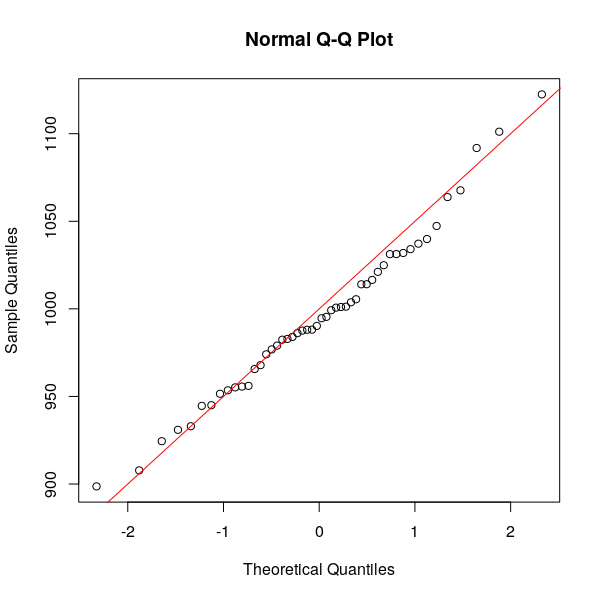
\includegraphics[width=.45\textwidth]{sampling-qqplot-good}
    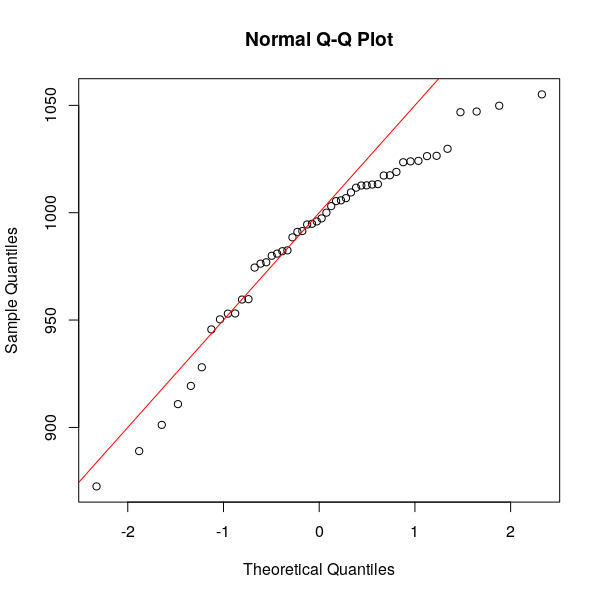
\includegraphics[width=.45\textwidth]{sampling-qqplot-bad}
  \end{center}
  \caption{The Q-Q plot on the left is based on a sample of 50 observations drawn from a normal distribution with mean 1000 and standard deviation 50. The plot on the right is based on a sample of 50 observations drawn from a Student's $t$-distribution with 15 degrees of freedom, with the same mean and standard deviation. The lines in red indicate where the observations should theoretically be situated. In the plot on the left, this is more or less the case, but on the right, especially in the extremes, observations deviate from the line.}
  \label{fig:qqplot}
\end{figure}

\lstinputlisting{data/qqplot.R}

\section{The Central Limit Theorem}
\label{sec:central-limit-theorem}

In this section, we'll discuss one of the most fundamental results in statistics and the foundation of sampling: the central limit theorem.

\begin{definition}[Linear combination of independent, identically distributed stochastic variables]
  Formal: A linear combination of a sufficiently large number of independent, identically distributed stochastic variables (i.e. with a well defined expected value and variance) will approximate the normal distribution, regardless of the underlying distribution.

  \[X_{i} \sim Nor(\mu_{i}, \sigma_{i}) \Rightarrow Y = \sum_{i} \alpha_{i} X_{i} \textnormal{ approximates the normal distribution} \]

  Consequently, the mean of a sample derived from a population with a random distribution will approximate a normal distribution for a sufficiently large value of $n$.
\end{definition}

Therefore, given a random sample of independent variables with a normal distribution,
the central limit theorem states that the mean of this sample will also approximate the normal distribution.
So, if you would repeatedly take a sample of the same size, and measure the mean, the resulting plot will approximate the graph of a normal distribution (cfr. Figure~\ref{sec:normal-distribution}).
The larger the sample, the closer the approximation will be.
The mean of the sample therefore has a normal distribution, independent of the underlying distribution of the metric from which a sample is taken. 

In general:

\begin{definition}[The Central Limit Theorem]
  Consider a random sample of $n$ observations drawn from a population with expected value $\mu$ and standard deviation $\sigma$.
  If $n$ is sufficiently large, the probability distribution of the sample mean $\overline{x}$ will approximate a normal distribution with expected value $\mu_{\overline{x}} = \mu$ and standard deviation $\sigma_{\overline{x}} = \frac{\sigma}{\sqrt{n}}$.
  The larger the sample, the better the probability distribution of $\overline{x}$ will approximate the expected value of the population, $\mu$.
\end{definition}

When taking a sample, the underlying distribution is rarely known, and yet one can make statements about the sample mean. This is entirely thanks to the central limit theorem, which imposes a rule about the mean regardless of the underlying probability distribution. 
The central limit theorem keeps the sample mean under control, locking it in the Gaussian cage from which it can never escape. This, and only this, allows scientists to study it carefully, observe it, and enables them to formulate conclusions.

Because, if the distribution of the sample mean would depend on the underlying distribution, which would be expected to some extent, it would be impossible to make concrete statements about many scientific results. 
In statistics theory, limits of sample means appear everywhere, and they can be easily replaced by a normal distribution thanks to the central limit theorem. 
If this would not be possible, the whole theory of estimating parameters would collapse, which would be disastrous in practice. 
Comparing research would be reduced to an almost impossible task, and statistics in general would become much more difficult and complicated.

The proof of the central limit theorem is outside the scope of this course, even though it is surprisingly easy to understand.

\subsection{Application of the Central Limit Theorem}
When drawing a random sample of a sufficiently large size $n$ form a population with an unknown $\mu$ and (known) standard deviation $\sigma$, the probability distribution of the sample mean is a stochastic variable $M \sim N (\overline{x}, \frac{\sigma}{\sqrt{n}})$.

\begin{example}
  Let's consider the reaction times of all our superheroes and assume we have drawn a random sample with $n = 100$, $\overline{x} = 90$, and $\sigma = 60$ (ms).
  We can then ask ourselves: what is the probability that the average reaction time of a superhero is below $104$ ms?

  \begin{enumerate}
    \item In this example, the stochastic variable is the average reaction speed $\overline{x}$ in a sample of $n=100$ superheroes. Because of the central limit theory, the following holds:
    \[ \overline{x} \sim Nor(\mu = 90, \sigma_{\overline{x}} = \frac{60}{\sqrt{100}} = 6) \]
    \item We can calculate the associated $z$-score:
    \[ z = \frac{104-90}{\frac{60}{\sqrt{100}}} = \frac{104-90}{6} = 2.33 \]
    \item And therefore: $P(\overline{x} < 104) = P(Z < 2.33) = 1 - 0.0099 \approx 0.99$ or about 99\%
  \end{enumerate}
\end{example}

\subsection{Estimating Stochastic Parameters}
\label{ssec:estimating-stochastic-parameters}

If we want to study a sample, it is usually to draw conclusions about the population as a whole. 
For example, we want to know the average strength of a superhero, or the fraction of rich superheroes. 
In general, we'll \emph{estimate} a parameter of the population based on the sample. For example, $\overline{x}$ is used as an estimate of $\mu$. This type of estimation is defined as:

\begin{definition}[point estimate]
  A \emph{Point Estimate}\index{estimate!point} for a population parameter is a formula or equation that allows us to calculate a value to estimate that parameter.
\end{definition}

Another type of estimates are \emph{interval estimates}\index{estimate!interval}, a.o.~confidence intervals. These are discussed in the next sections.

\subsection{Confidence interval for the population mean of a large sample}
\label{ssec:confidence-interval-pop-mean-large-sample}

When we estimate the population mean from a sample, we have no idea how correct this estimate is. However, the properties of the normal distribution allow us to construct an interval that will contain the population mean with the desired level of confidence.

\begin{definition}[Confidence Interval]
  A \emph{Confidence Interval}\index{confidence interval} is an equation or formula that allows us to construct an interval that will contain the parameter to be estimated with a certain level of confidence.
\end{definition}

An initial estimate for the population mean is of course the sample mean:

\[ \overline{x} = \frac{1}{n} \sum_{i} x_{i} \]

Of course this estimate is not the real population mean. However, because of the central limit theorem, we know that the mean of a sample of size $n$ is normally distributed with mean $\mu$ and standard deviation $\frac{\sigma}{\sqrt{n}}$.
After standardisation, we get:
\[ Z = \frac{\overline{x} - \mu}{\frac{\sigma}{\sqrt{n}}} \]

This expression depends on $\mu$, but we know that this parameter has a normal distribution. As a result, we can find limits $-z$ and $z$, independent from $\mu$, that will contain $Z$ with a \emph{confidence level} $1 - \alpha$ (which can be chosen by the researcher). In this example, we choose $1 - \alpha= 0.95$ (and consequently $\alpha = 0.05$).

\[P(-z < Z < z) = 1 - \alpha = 0.95 \]

After applying the rule of symmetry, we find that we need to determine $z$ by:

\[ P( Z < z) = 1 - 0,025 = 0.975 \]

When we look this up in a Z-table, we'll find that $z = 1.96$. Or, alternatively, we can calculate \verb|qnorm(0.975)| in R.

The confidence interval then is:

\[ P( -1.96 < \frac{\overline{x} - \mu}{\frac{\sigma}{\sqrt{n}}} < 1.96 ) = 1 - \alpha\]

and therefore
\[ P ( \overline{x} -1.96 \frac{\sigma}{\sqrt{n}} <\mu < \overline{x} + 1.96 \frac{\sigma}{\sqrt{n}}) = 1 - \alpha \]

Using this technique, we can determine the bounds of an interval that will contain $\mu$ with a confidence level of 95\%. 
If you would repeatedly draw a sample from this population and calculate the confidence interval around $\overline{x}$, then in 95\% of the cases, we expect the actual $\mu$ to be inside the interval bounds.

However, note that we assume to know the standard deviation of the population, which will generally not be the case. If the sample size is sufficiently large, the standard deviation of the sample is used as a point estimate for the standard deviation of the population.

\[ P ( \overline{x} -1,96 \frac{\sigma_{\overline{x}}}{\sqrt{n}} < \mu < \overline{x} + 1,96 \frac{\sigma_{\overline{x}}}{\sqrt{n}}) = 1 - \alpha \]


\begin{figure}
\centering
\begin{tikzpicture}
\begin{axis}[
  domain=-3:3, samples=100,
  axis lines*=left, xlabel=$z$,
  every axis y label/.style={at=(current axis.above origin),anchor=south},
  every axis x label/.style={at=(current axis.right of origin),anchor=west},
  height=5cm, width=12cm,
  xtick={-1.96,0,1.96}, ytick=\empty,
  enlargelimits=false, clip=false, axis on top,
  grid = major
  ]
  \addplot [fill=cyan!20, draw=none, domain=-3:3] {gauss(0,1)} \closedcycle;
  \draw [yshift=-0.6cm, latex-latex](axis cs:-1.96,0) -- node [fill=white] {$\sigma$} (axis cs:1.96,0);
\end{axis}
\end{tikzpicture}
\caption{Standard normal distribution with a 95\% confidence interval.}
\label{fig:verdelingStandaardnormaal}
\end{figure}

\subsection{Confidence interval for the population mean of a small sample}
\label{ssec:confidence-interval-pop-mean-small-sample}

In the case of a small sample, we can no longer assume that the probability distribution of $\overline{x}$ approximates the normal distribution. 
The central limit theorem only holds for large sample sizes of about $n > 30$.

The shape of the probability distribution of $\overline{x}$ now depends of the shape of the underlying probability distribution of the population. 
Although $\sigma_{\overline{x}} = \frac{\sigma}{\sqrt{n}}$ still holds, the standard deviation of the sample $s$ 
could be a bad estimate for $\sigma$ if the sample is small.

However, there is a solution in the form of the so-called Student's $t$-distribution. Instead of calculating the z-score:
\[ z = \frac{\overline{x} - \mu}{\frac{\sigma}{\sqrt{n}}} \]

we can use the $t$-score:
\[ t = \frac{\overline{x} - \mu}{\frac{s}{\sqrt{n}}} \]

The probability density of the Student's $t$-distribution is very similar to the standard normal distribution: 
bell-shaped, symmetrical, and with an expected value of 0.

The exact shape depends on the sample size $n$, or more precisely on the degrees of freedom\index{degrees of freedom} $(n-1)$ (abbreviated as $df$).

Note that:
\begin{itemize}
  \item $(n-1)$ is also used to calculate the sample variance $s^{2}$;
  \item When $n \rightarrow \infty$ this converges to the standard normal distribution.
\end{itemize}

To calculate a confidence interval for a sample with a small number of observations, we need to do the following:

\begin{definition}[Confidence Interval for a Small Sample]
  To determine a confidence interval for the average based on a small sample, we calculate:
  \[ \overline{x} \pm t_{\frac{\alpha}{2}}(\frac{s}{\sqrt{n}}) \]
  in which $t_{\frac{\alpha}{2}}$ is based on $(n-1)$ degrees of freedom. 
  We still assume that the sample is random and drawn from a population that is approximately normally distributed.
\end{definition}

\begin{table}
  \centering
  \begin{tabular}{ll}
    \textbf{Function}     & \textbf{Description}                                      \\
    \midrule
  	\verb|pt(x, df)| & Left tail probability, $P(X<\mathtt{x})$                       \\
  	\verb|dt(x, df)| & Altitude of the Gaussian curve at point \texttt{x}             \\
  	\verb|qt(p, df)| & What boundary value contains \texttt{p}\% of the observations? \\
  	\verb|rt(n, df)| & Generate \texttt{n} random numbers using the $t$ distribution  \\ 
  \end{tabular}

  \caption{Functions for calculating the probability in R for the Student's $t$-distribution with \texttt{df} degrees of freedom, expected value 0 and standard deviation 1.}
  \label{tab:t-prob-r}
\end{table}

\subsection{Confidence interval for a population fraction of a large sample}
\label{ssec:confidence-interval-pop-fraction-large-sample}

If you want to measure a variable as a fraction, for example the percentage of people that responded with ``yes'' to a specific question, this is equivalent to estimating the probability $p$ on success in a binomial experiment, i.e.~an experiment with a sample space consisting of two elements, ``success'' and ``failure''. 
If the probability of ``success'' is $p$, the probability of ``failure'' is $q = 1 - p$. 
The value of $p$ can be estimated based on the sample:

\[ \overline{p} = \frac{\textnormal{number of successes}}{n} \]

In order to calculate a confidence interval for $\overline{p}$, we need to know the probability distribution of $\overline{p}$. 
The central limit theory can then be applied to the average number of successes in a sample of size $n$. 
If success = 1 and failure = 0, we have a sample of $n$ elements, each having the same distribution (probability of 1 is $p$ and probability of 0 is $q=1-p$).
The probability distribution of $\overline{p}$ has the following properties:

\begin{itemize}
  \item The expected value of the probability distribution of $\overline{p}$ is $p$.
  \item The standard deviation of the probability distribution of $\overline{p}$ is $\sqrt{\frac{pq}{n}}$.
  \item For large samples, $\overline{p}$ is approximately normally distributed.
\end{itemize}

Since $\overline{p}$ is the sample mean of the number of successes, this allows us to calculate a confidence interval, analougous to the one for $\mu$ for large samples.

\begin{definition}[Confidence interval for $p$ for a large sample]
  \[ \overline{p} \pm z_{\frac{\alpha}{2}} \sqrt{\frac{\overline{p}\overline{q}}{n}} \]
  with $\overline{p} = \frac{x}{n}$ and $\overline{q} = 1- \overline{p}$
\end{definition}


\section{R}
We take a look at some basic operations related to several probability distributions.
Although R knows many different distributions, we will only focus on the main ones.
To find out all supported distributions, you can use the following command in R:

\begin{lstlisting}
> help.search ("distribution")
\end{lstlisting}

In this section we will provide some details about the command used for a normal distribution, and briefly mention the command for other distributions.
The functions for the different distributions are very similar.

The prefixes are as follows:
\begin{description}
	\item[d] returns the altitude of the selected curve
	\item[p] returns the cumulative probability density function
	\item[q] returns the reverse cumulative density function
	\item[r] returns a random value
\end{description}

\subsection{The Normal Distribution}
There are four functions to generate values associated with the normal distribution.
\subsubsection{dnorm}

When a value is provided, this function returns the height of the probability distribution for each requested point.
If no other parameters are provided, without mean or standard deviation, the standard normal distribution is used (with mean 0 and standard deviation 1).
However, it is also possible to use a different value for the average and standard deviation by adding the corresponding parameters.

\lstinputlisting{data/norm.R}

\subsubsection{pnorm}

This function returns the cumulative probability density function, or in other words the left tail probability: \texttt{pnorm(x)} is $P(Z < x)$.

\subsubsection{qnorm}
The function \texttt{qnorm} is the inverse of \texttt{pnorm}.
The main idea behind \texttt{qnorm} is that when you provide a probability $\alpha$, 
this function returns the value for which the left tail probability is $\alpha$.

\lstinputlisting{data/qnorm.R}

\subsubsection{rnorm}

The \texttt{rnorm} function can generate random values using a normal distribution.
The first argument is the required number of values, and a custom average and standard deviation can also be supplied as optional parameters.

\lstinputlisting{data/rnorm.R}




% Exercises 
\section{Exercises}
\label{sec:sampling-exercises}

\begin{exercise}
  \label{ex:prob-norm-dist}
  Calculate the following probabilities, either using a $z$ table, or using the appropriate R function. Also draw a sketch of the area.
  \begin{enumerate}[label=\alph*.]
    \item $P(Z < 1.33)$
    \item $P(Z > 1.33)$
    \item $P(Z < -1.33)$
    \item $P(Z > -1.33)$
    \item $P(Z < 0.45)$
    \item $P(Z > -1.05)$
    \item $P(Z < 0.65)$
    \item $P(-0.45 < Z < 1.20)$
    \item $P(-1.35 < Z < -0.10)$
    \item $P(-2.10 < Z < -0.90)$
  \end{enumerate}
\end{exercise}

\begin{exercise}
  Determine the probability distribution and the cumulative probability curve for a normal distribution with mean $\mu = 2.5$ and standard deviation $\sigma = 1.5$.
  Determine the area of the surface below the density curve between $ x = 0.5 $ and $ x = 4 $.
  Verify your answer by doing the calculation.
\end{exercise}

\begin{exercise}
  Determine the probability distribution and cumulative probability curve for a $t$-distribution with $df = 3$.
  Also draw a normal distribution with $\mu = 0$ and $\sigma = 1$.
\end{exercise}

\begin{exercise}
  Use the \verb|rnorm()| function to generate a random sample of 25 values based on a normal distribution with mean $\mu = 0$ and standard deviation $\sigma = 1$.
  Draw a histogram, using \verb|probability = TRUE|.

  Draw an overlay on the histogram consisting of (a) the theoretical probability distribution curve of a normal distribution with mean $\mu = 0$ and standard deviation $\sigma = 1$;
  and (b) an ``estimated'' probability distribution curve based on the measured sample mean and standard deviation.

  Repeat this for a sample consisting of 100 and 500 values.
\end{exercise}

\begin{exercise}

  The course of research techniques at a college is organised in two separate classes. 
  Students were distributed at random over the two classes, A and B, so we can assume that one class is not significantly better than the other. 
  Class A is lectured by Mrs. X, class B by Mr. Y.

  Mrs. X is rather strict and her group gets grades with an average of 54/100 and a standard deviation of 11.

  Y is less strict and is known for stimulating his students by giving them a bonus point at times. By the end of the academic year, the grades for his group have an average of 62/100 with a standard deviation of 7.

  Wouter is a student of class A and got a grade of $\frac{63}{100}$, Stijn from class B got $\frac{67}{100}$. Who has the best result?
\end{exercise}

\begin{exercise}
  A survey conducted between 1988 and 1994 indicated that the average cholesterol level of women between 20 and 29 years was 183 mg/dl, with a standard deviation of 36. 
  The sample consisted of 81 women, and we assume that the sample was taken at random.

  \begin{enumerate}[label=\alph*.]
    \item Plot the probability distribution for the sample mean $\overline{x}$.
    \item What is the probability that $\overline{x}$ is smaller than 185?
    \item What is the probability that $\overline{x}$ is between 175 and 185?
    \item What is the probability that $\overline{x}$ is larger than 190? 
  \end{enumerate}
\end{exercise}

\begin{exercise}
  A random sample consisting of 64 observations is drawn from a population with an unknown distribution. 
  However, the population mean and standard deviation are known: $\mu = 20$ and $\sigma = 16$.

  \begin{enumerate}[label=\alph*.]
    \item What are the mean and standard deviation of the sample?
    \item Describe the shape of the probability distribution of the sample mean. Does this depend on the sample size?
    \item Calculate the $z$-score for $\overline{x_{1}} = 15.5$ and $\overline{x_{2}} = 23$.
    \item Calculate the probability that $\overline{x} < 16$.
    \item Calculate the probability that $\overline{x} > 23$.
    \item Calculate the probability that $16 < \overline{x} < 22$.
  \end{enumerate}
\end{exercise}

\begin{exercise}
  Speed bumps are designed to influence the speed of drivers. 
  Depending on the desired speed in a street, speed bumps can be made steeper or more gradual.
  Speed bump A is designed so that 85\% of drivers pass over with a maximum speed of 50 km/h. 
  The speed of the drivers appears to be normally distributed. A sample indicates that the average speed is 43.1 km/h with a standard deviation of 6.6 km/h.

  \begin{enumerate}[label=\alph*.]
    \item Prove that 85\% of drivers actually do not drive faster than 50 km/h.
    \item If the sample size was 1200, what is the expected probability of a driver passing with a speed of at least 55 km/h?
  \end{enumerate}
\end{exercise}

\begin{exercise}
  Lately, a canned goods manufacturer received complaints about the net contents of their carrot and peas cans. 
  According to the label, the can should contain 1 liter. 
  To verify these complaints, the QA department draws a random sample of 40 cans and checks the contents. 
  The results are provided in Table~\ref{tab:canned-goods-sample-values}.

  A. Add the following data to the table:
  \begin{itemize}
    \item the cumulative absolute frequency
    \item the relative frequency
    \item the cumulative relative frequency
  \end{itemize}

  B. Calculate:
  \begin{itemize}
    \item The mean and standard deviation of the sample
    \item The percentage of cans for which the contents are too low
    \item Plot a histogram of the absolute frequency
    \item Are the observations normally distributed? How can you determine this?
  \end{itemize}
\end{exercise}

\begin{table}
  \centering
  \begin{tabular}{lr}
    \toprule
    Contents & $n_{i}$ \\
    \midrule
    $[970,980[$ & 3 \\
    $[980,990[$ & 5 \\
    $[990,1000[$ & 13 \\
    $[1000,1010[$ & 11 \\
    $[1010,1020[$ & 5 \\
    $[1020,1030[$ & 3 \\
    \bottomrule
  \end{tabular}
  \caption{Sample Values}
  \label{tab:canned-goods-sample-values}
\end{table}

\begin{exercise}
  Confidence intervals.
  
  \begin{enumerate}
    \item What are the lower and upper boundary values for a confidence interval of 99\%?
    \item A confidence interval of 99\% is wider than a confidence interval for 95\%. Why?
    \item What would a confidence interval of 100\% look like?
  \end{enumerate}
  
\end{exercise}

\begin{exercise}
  \label{ex:confidence-money}
  
  Import the dataset \texttt{money.csv} in R. 
  We assume that the values of this sample are normally distributed with 
  an unknown population mean $\mu$, but the standard deviation of the population
  is supposed to be known; $\sigma = 99$. 
  
  \begin{enumerate}
    \item Determine a 99\% confidence interval for the population mean.
    \item Determine a 95\% confidence interval for the population mean.
    \item Suppose that $\sigma$ is also unkown. In this case, determine a 95\% confidence interval for the population mean.
    \item Determine a 95\% confidence interval for the population mean, assuming that the sample consists of only the 25 first values of the imported file.
  \end{enumerate}
\end{exercise}

\begin{exercise}
  A web hosting company has a Service Level Agreement with a customer that guarantees an uptime of ``five nines'' (99.999\%). 
  This is verified at the end of each year and if the minimal uptime is not met, a fine is imposed.

  To measure the uptime, a monitoring system queries the web server every minute using a \texttt{HTTP GET /} request and verifies the result using the HTTP return code. 
  In january, a single HTTP request was unsuccesful.

  \begin{itemize}
    \item If the current trend continues, what is the probability that the SLA is not met at the end of the year? Use the formula for the probability distribution of a fraction.
    \item In this particular case, the formula actually isn't suitable, and gives a slightly distorted result. Why?
  \end{itemize}
\end{exercise}






% Answers
\section{Solutions to selected exercises}
\label{sec:oplossingen-steekproefonderzoek}

\paragraph{Exercise \ref{ex:prob-norm-dist}}

\begin{enumerate}[label=\alph*.]
  \item $0.908$
  \item $0.092$
  \item $0.092$
  \item $0.908$
  \item $0.674$
  \item $0.853$
  \item $0.742$
  \item $0.559$
  \item $0.372$
  \item $0.166$
\end{enumerate}

\paragraph{Exercise \ref{ex:confidence-money}}

\begin{enumerate}
  \item $[481.725; 523.368]$
  \item $[486.704; 518.390]$
  \item $[486.476; 518.617]$
  \item $[485.761; 519.332]$
\end{enumerate}

   
\chapter{Testing Procedures}
\label{ch:testing-procedures}

In previous chapters we introduced an approach for estimating certain key metrics about a population based on a sample, for example using point estimators or confidence intervals.
We can also use this information to test certain hypotheses about a population. A hypothesis is an assumption that has yet to be proven.
The purpose of a testing procedure is to test a hypothesis regarding the value of 1 or more population parameters.

\begin{definition}[Statistical Hypothesis]
  A statistical hypothesis\index{hypothesis!statistical} is a statement about the numerical value of a population parameter.
\end{definition}

Examples of hypotheses:

\begin{itemize}
  \item On average, a superhero rescues at least 3.3 people a day.
  \item The average height of a superhero is at least 120 cm.
  \item \dots
\end{itemize}

In this chapter we will formulate the general theory of testing using hypotheses about the population mean $\mu$, the $Z$-test.
Apart from the $Z$-test, there are many other statistical hypothesis tests that can be used in specific cases.
The most appropriate statistical test depends, among other things, on the population size in question (average, standard deviation, etc.),
and assumptions regarding the underlying stochastic distribution of the population (normally distributed or not, etc.).

\section{Learning Goals}
\label{sec:testing-procedures-learning-goals}

By the end of this chapter you must be able to:

\begin{itemize}
  \item Explain the following concepts:
  \begin{itemize}
    \item hypothesis test, statistical hypothesis, null hypothesis, alternative hypothesis;
    \item test statistics, region of acceptance, region of rejection / critical region, probability value;
    \item $Z$-test, $t$-test, left tail, right tail, two tail;
    \item Type I and Type II errors;
  \end{itemize}
  \item Describe the general procedure for a statistical test;
  \item Based on the description of a situation in which you are asked to verify a statement about the population mean:
  \begin{itemize}
    \item to determine whether a $z$- or $t$-test could be used;
    \item to deduce from the research question whether the left, right of two tail variant should be used;
  \end{itemize}
  \item To correctly apply the $z$- or $t$-test for a given situation, i.e.:
  \begin{itemize}
    \item Formulate the null and alternative hypotheses (mathematical notation);
    \item Calculate the test statistic
    \item Calculate the critical value(s) and determine whether the test statistic is inside the region of acceptance or rejection;
    \item Calculate the probability value;
    \item Formulate a correct conclusion (reject null hypothesis or not);
    \item Formulate an answer to the research question.
  \end{itemize}
\end{itemize}

\section{Elements of a hypothesis test}
\label{sec:elements-hypothesis-test}

In general, a testing procedure consists of 4 elements:
\begin{enumerate}
  \item \textbf{Null Hypothesis}\index{null hypothesis}\index{hypothesis!null} $H_{0}$: We will try to disprove this hypothesis using proof by contradiction. We will accept this hypothesis, unless observations from the sample convincingly point to the contrary.
  \item \textbf{Alternative hypothesis}\index{hypothesis!alternative} $H_{1}$: In general, this is the hypothesis the researcher wants to prove. However, this hypothesis will only be accepted if the observations from the sample convincingly indicate its correctness.
  \item \textbf{Test Statistic}: The variable that is derived from the sample
  \item Region of acceptance and region of rejection / critical region:
  \begin{itemize}
    \item \textbf{Region of Acceptance\index{region of acceptance}}: The region of values supporting the null hypothesis $H_{0}$
    \item \textbf{Region of Rejection\index{region of rejection}}: The region containing the values that reject the null hypothesis. Also referred to as critical region\index{region!critical}.
  \end{itemize}
\end{enumerate}

An alternative for the last step is calculating the \emph{probability value} (see further).

The decision to reject or accept the null hypothesis $H_{0}$ is based on information from a sample, drawn from a population on which the hypothesis is based.
The sample values are used to calculate a single value of a test statistic that will determine the decision. 
To this end, all possible values for the test statistic are divided into two regions, the region of acceptance and the region of rejection.
If the value of the test statistic is inside the region of rejection, the null hypothesis is rejected and the alternative hypothesis accepted.
If the value of the test statistis is inside the region of acceptance, the null hypothesis is accepted.

\section{Testing Procedure for the \texorpdfstring{$z$}{z}-test}
\label{sec:testing-procedure-z-test}

For the first test procedure we will discuss in this course, we will verify a statement about the population mean $\mu$.
This test procedure is commonly known as the $Z$-test\index{$Z$-test}\index{test!$Z$}.

\begin{enumerate}
  \item The suspicions about the population are described using two hypotheses $H_{0}$ and $H_{1}$. For the (right-tail) $Z$-test the null hypothesis states that the population mean $\mu$ has a certain value, and the alternative hypothesis states that $\mu$\ is \emph{greater} than this value.
  \item The significance level\index{significance level}\index{level!significance} $\alpha$ and sample size $n$ are determined. In principle, you can choose a value for $\alpha$ (e.g. 0.05)\footnote{Note that the significance level is related to the confidence interval $1-\alpha$, cfr. Section~\ref{ssec:confidence-interval-pop-mean-large-sample}}. The closer the significance level is to 0, the less doubt there is about the result of the test, but on the other hand it becomes more difficult to reject the null hypothesis.
  \item The value of the test statistic for the sample is calculated. The result determines whether we can reject the null hypothesis $H_{0}$ or not. Thanks to the central limit theorem we know that the probability distribution of the sample mean is normally distributed, $M \sim Nor( \mu, \frac{\sigma}{\sqrt{n}})$.
  \item We determine the critical region, or more specifically the boundary between the region of acceptance and the region of rejection. We look for a critical value $g$ so that:
  
  \begin{align}
  P(M > g) = \alpha & \Leftrightarrow P\left(Z> z=\frac{g-\mu}{\sigma/\sqrt{n}}\right) = \alpha & \mathrm{(standardization)}\\
  & \Leftrightarrow P\left(Z < z = \frac{g-\mu}{\sigma/\sqrt{n}}\right) = 1-\alpha & \mathrm{(100\%-rule)}
  \end{align}
  
  The $z$-value depends on the chosen significance level, and can be found using a $z$-table or calculated using the R function \texttt{qnorm(1-alpha)}. From this we can derive $g$:
  
  \begin{equation}
  z = \frac{g-\mu}{\sigma/\sqrt{n}} \Leftrightarrow g = \mu + z \frac{\sigma}{\sqrt{n}}
  \label{eq:critical-calue-z-test}
  \end{equation}

  All values \emph{left} of $g$ form the region of acceptance. Value on the right, which are far away from the assumed population mean $H_0$, form the region of rejection, cfr. Section~\ref{sec:critical-region}.
\end{enumerate}

\begin{example}
  \label{ex:hypothesis-test-daily-rescues}
  In general we assume that superheroes rescue 3.3 people per day on average. However, researchers are getting the feeling that this is not the case: they have the impression that a superhero rescues \emph{more} than $3.3$ people per day.

  The researchers want to to investigate this and take a sample of $n = 30$ superheroes. For this sample, the sample mean is $\overline{x} = 3,483$. The standard deviation of the population is assumed to be known and is equal to $\sigma = 0.55$.
  
  Using these results, can the researchers conclude that superheroes rescue on average more than 3.3 people per day?

  \begin{enumerate}
    \item We assume that the number of people a superhero rescues on average is normally distributed and formulate two hypotheses regarding the parameter $\mu$.
    \begin{itemize}
      \item $H_{0}$ = the null hypothesis (that we want to reject). In this case: \[ H_{0} : \mu = 3.3 \]
      \item $H_{1}$ = alternative hypothesis (suspect that we want to prove). In this case: \[H_{1}= \mu > 3.3 \]
    \end{itemize}
  
    We initially assume that the null hypothesis $H_{0}$ is true. If the average number of people rescued per day of the sample ($\overline{x}$) differs a lot from the assumed value, we reject the null hypothesis $H_{0}$ and accept the alternative hypothesis $H_{1}$.

    But how do we define ``differs a lot''? Would it be easy to draw a sample with a mean of $3.483$ based on a population with a mean of $3.3$? The central limit theorem (cfr. Section~\ref{ch:central-limit-theorem}) allows for calculating the probability of this.
    
    \item Determine significance level $\alpha$ and sample size $n$. We want to have a significance level of 5\%, so $\alpha = 0.05$. The sample size is provided for this case, and is equal to $n = 30$.
    
    \item Calculate the value of the test statistic in the sample. For this example, we take the sample mean: $\overline{x} = 3.483$
    
    We assume that the null hypothesis $H_{0}$ is true and that we have a good estimate for $\sigma$ ($\sigma = 0,55$). Then, according to the central limit theorem, we can say about the sample mean $M$ that:

    \[M \sim  Nor(\mu = 3.3; \sigma = \frac{0.55}{\sqrt{30}})\]

    The value $\overline{x} = 3,483$ is located on the far right (see Figure~\ref{fig:hypothesis-test-daily-rescues}). $\overline{x} $ is so far to the right that the probability to get this or a greater value, is very small (if $H_{0}$ is true). As a result, it is very difficult to explain such a value based on mere coincidence. Intuitively we feel that the further the observed value of $\overline{x}$ is located in the right direction, the more inclined we are to reject the null hypothesis. But what is too far and what is not?
    
    \item Calculate the critical value. The $z$=value for a significance level of $0,05$ equals 1.654\footnote{This can be calculated in R using \texttt{qnorm(1 - 0.05)}}.
    
    \[ g = \mu + z \times \frac{\sigma}{\sqrt{n}} = 3.3 + 1.645 \times \frac{0.55}{\sqrt{30}} \approx 3.45 \]
    
    The sample mean $\overline{x} = 3.483 $ is even further away from $\mu = 3.3$ than the limit value $g = 3.45$. It is therefore very unlikely that such a sample can be drawn from a population with this average. Such an event will only occur in 34 samples out of 1000. In other words, the sample value is in the rejection area. Because of this, we can reject $H_0$ and conclude that superheroes indeed rescue \emph{more} than 3.3 people a day.

  \end{enumerate}

\end{example}

\begin{exercise}
  Can we assume in Example~\ref{ex:hypothesis-test-daily-rescues} that the mean has a normal distribution? Why (not)?
\end{exercise}

\begin{figure}
  \centering
  \begin{tikzpicture}
    \begin{axis}[
        domain=3:3.6, samples=100,
        axis lines*=left, xlabel=$x$,
        every axis y label/.style={at=(current axis.above origin),anchor=south},
        every axis x label/.style={at=(current axis.right of origin),anchor=west},
        height=5cm, width=12cm,
        xtick={3.3,3.483}, ytick=\empty,
        xticklabels={$\mu$,$\overline{x}$},
        enlargelimits=false, clip=false, axis on top,
        grid = minor
      ]
      \addplot [fill=cyan!20, draw=none, domain=3:3.465] {gauss(3.3,0.1004)} \closedcycle;
      \addplot [fill=none, draw=black, domain=3:3.6] {gauss(3.3,0.1004)} \closedcycle;
      \draw [-](axis cs:3.465,1.6) -- (axis cs:3.465,0);
      \node at (axis cs:3.465,1.8) {3.465};
      \node at (axis cs:3.483,-0.7) {3.483};
      \node at (axis cs:3.3,-0.7) {3.3};
    \end{axis}
  \end{tikzpicture}
  \caption{Distribution of the number of people rescued by a superhero on average per day (Example~\ref{ex:hypothesis-test-daily-rescues}). The probability distribution of the sample mean is normally distributed with $\mu = 3.3$ and $\sigma = 0.55$. The sample mean is $\overline{x} = 3.483$. The critical value for acceptance/recjection of $H_{0}$ is 3.465.}
  \label{fig:hypothesis-test-daily-rescues}
\end{figure}

\section{Critical Region}
\label{sec:critical-region}

The formula for calculating the critical value (cfr. Equation~\ref{eq:critical-calue-z-test}) is based on the central limit theorem, and in particular on confidence intervals.

The critical value defines a confidence interval around $\mu$ for a selected significance level. For example, if we assume that $\alpha = 0.05$, the central limit theorem states that if we repeatedly take enough samples from this population, we can expect that in 95\% of cases the sample mean will be located within this confidence interval.

If we reverse this reasoning, and took a sample for which the mean $\overline{x}$ is \emph{not} located within this confidence interval, then the chance is very small (less than 5\%) that the sample has been drawn from a population with assumed mean $\mu$. Therefore, in this case we can reject the null hypothesis.

In Example~\ref{ex:hypothesis-test-daily-rescues} the critical value is the value of $g$ for which:

\[ P(M > g) = \alpha \]

This can be converted to:

\[ P(Z > \frac{g - \mu}{\frac{\sigma}{\sqrt{n}}}) = \alpha \]

And as a result:

\begin{equation}
  \label{eq:critical-value-right-tail}
  g = \mu + z \times \frac{\sigma}{\sqrt{n}}
\end{equation}

\section{Probability Value}
\label{sec:probability-value}

A characteristic that is often used to show how strongly the observed value deviates from $H_{0}$ is the probability value (also known as $p$-value\index{$p$-value}). This is an alternative way to determine whether the null hypothesis can be rejected or not.

\begin{definition}[probability value]
  The \emph{probability value}\index{probability value} is the probability, if the null hypothesis is true, to obtain a value for the test statistic that is at least as extreme as the observed value.
\end{definition}

\begin{definition}[statistical significance]
  In statistical hypothesis testing, a result has a \emph{statistical significance}\index{significance} when the observed probability value $p$ of the test statistic is lower than the significance level $\alpha$.
  A $p$-value below the selected signifance level is considered to be too extreme to hold to the assumption that the null hypothesis is true.
\end{definition}

\begin{example}
  In the research regarding the daily number of rescues by superheroes (cfr. Example~\ref{ex:hypothesis-test-daily-rescues}) the probability value can be calculated as follows:
  
  \[ P(M > 3.483) = P \left(Z> \frac{3.483 - 3.3}{\frac{\sigma}{\sqrt{n}}}\right) = P (Z > 1.822) = 0.0344 \]
\end{example}

If the probability value (or $p$-value) is less than the significance level, $H_{0}$ is rejected, if the $p$-value is equal or greater than $\alpha$ we cannot reject $H_{0}$.
In our example the $p$-value is $0.0344$, which is less than $\alpha = 0.05$, so we have to reject $H_{0}$.

\begin{itemize}
  \item $p$-value $< \alpha \Rightarrow$ reject $H_{0}$, because the obtained value for $\overline{x}$ is too extreme;
  \item $p$-value $\geq \alpha \Rightarrow$ not rejecting $H_{0}$, because the obtained value for $\overline{x}$ can still be explained by coincidence.
\end{itemize}

\section{One- or two-tailed tests}
\label{sec:one-or-two-tailed-tests}

Example~\ref{ex:hypothesis-test-daily-rescues} focuses on a hypotheses where we suspect that the population mean is \emph{greater than} a certain value. We doubt the correctness of the null hypotheses if our sample mean is significantly greater than the target average $\mu = 3.3; \alpha = 0.05$. The critical region to reject $H_{0}$ is on the right side of the curve and therefore we call this test right-tailed.

We could also create a test in which we suspect that the superheroes on average rescue \emph{fewer} people a day. In this case, the critical region is on the left side of the curve and we call this test left-tailed.

\begin{exercise}
  \label{ex:critical-value-left-tail}
  
  What would you have to change in Equation~\ref{eq:critical-value-right-tail} in order to calculate a correct value for a left-tailed $Z$-test?
\end{exercise}

Sometimes it might be necessary to perform a two-tailed test. 
In this case, the alternative hypothesis states that the population mean is different from a certain value.
Two critical values must then be calculated, namely the left and right value:

\begin{equation}
  g = \mu \pm z \times \frac{\sigma}{\sqrt{n}}
  \label{eq:critical-value-two-tailed}
\end{equation}

The critical region has a total area of $1 - \alpha$, and consists of two regions with an area of $\alpha / 2$, one on the left and one on the right.
We therefore have to pick the corresponding $z$-values. For example, if the significance level $\alpha = 0.05$, we look for the $z$-value for which:

\[P(Z < -z) + P(Z > z) = \alpha \Leftrightarrow 2 P(Z>z) = \alpha \Leftrightarrow P(Z < z) = 1-\frac{\alpha}{2} = 0,975\]

The corresponding $z$-value is about $1.96$ (can be found in the $z$-table or in R by using \texttt{qnorm(.975)}).

The three types of the $Z$-test are summarized in Table~\ref{tab:z-test-types}.

\begin{table}
  \centering
  \begin{tabular}{l|ccc}
    \toprule
    Goal              & \multicolumn{3}{l}{\parbox{.5\textwidth}{Test a statement regarding the mean of the population $\mu$ by using a sample of $n$ random values}} \\
    \midrule
    Condition         & \multicolumn{3}{l}{\parbox{.5\textwidth}{The population has a random distribution, $n$ is sufficiently large}} \\
    \midrule
    Test Type         & Two-Tailed           & Left-Tailed     & Right-Tailed     \\
    \midrule
    $H_{0}$           & $\mu = \mu_{0}$      & $\mu = \mu_{0}$ & $\mu = \mu_{0}$  \\
    $H_{1}$           & $\mu \neq \mu_{0}$   & $\mu < \mu_{0}$ & $\mu > \mu_{0}$  \\
    Critical Region   & $\left|z\right| > g$ & $z< -g $        & $z>g$            \\
    Test Statistic    & \multicolumn{3}{c}{$z = \frac{\overline{x} - \mu_{0}}{\frac{\sigma}{\sqrt{n}}}$} \\
    \bottomrule
  \end{tabular}
  \caption{Summary of the different types of the $Z$-test.}
  \label{tab:z-test-types}
\end{table}

\section{The \texorpdfstring{$z$}{z}-test in R}
\label{sec:z-test-R}

The code example below is the elaboration of Example~\ref{ex:hypothesis-test-daily-rescues} in R.

\lstinputlisting{data/z-test.R}

\begin{figure}
  \centering
  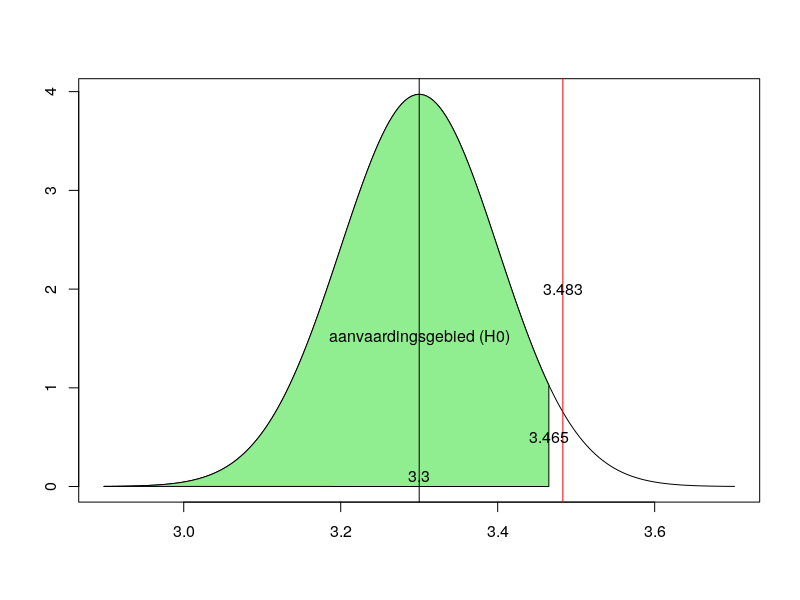
\includegraphics[width=\textwidth]{z-toets-reddingen}
  \caption{R Plot for the case study of Example~\ref{ex:hypothesis-test-daily-rescues}}
\end{figure}

\section{Examples}
\label{sec:testing-procedures-examples}

\begin{example}
  For a random sample consisting of 50 observations we have that:
  \begin{itemize}
    \item $\overline{x} = 25$
    \item $s = \sqrt{55} = 7,41$
  \end{itemize}
  
  We want to find out if there is a reason to assume that the popolation mean $\mu$ is smaller than 27.
  
  \begin{enumerate}
    \item Formulate both hypotheses. 
    
    $H_{0} : \mu = 27$ and $H_{1}: \mu < 27$.
    
    \item Determine significance level $\alpha$ and sample size $n$.
    
    $\alpha = 0.05$ and $n=50$.
    
    \item Calculate the value of the test statistic.
    
    For this we select the sample mean $M$. According to the central limit theorem, we have that:
    
    \[ M \sim Nor(\mu = 27, \frac{\sigma}{\sqrt{n}}) \]
    
    The test statistic is:
    \[ Z = \frac{\overline{x} - \mu}{\frac{\sigma}{\sqrt{n}}} = \frac{25-27}{\sqrt\frac{55}{50}} \approx -1.91\]
    
    \item Calculate the critical value.
    
    We discover a critical value for the mean of \texttt{pnorm(-1.91)} or about $0.0281$. Given a significance level of 0.05, this indicates that we can reject $H_{0}$.
    
    \item Calculate and plot the critical region.
    
    \[ g = \mu - z \times \frac{\sigma}{\sqrt{n}} \]
    
    and therefore:
    
    \[ g = 27 - 1.645 \times \sqrt{\frac{55}{50}} \]
    \[ g =  25.27470944 \]
    
    We discover that $\overline{x} < g$, and therefore we can make the same conclusion, to reject $H_{0}$.
    
  \end{enumerate}
\end{example}

\begin{example}
  In a reseach about the amount of change in the pockets of our superheroes, researchers state that on average a superhero carries 25 euro of cash.
  They assume that the population variance $\sigma = 7$.
  For a random sample of size $n=64$, the average amount of money a superhero carries is $\overline{x} = 23$ euro. 
  For the significance level, $\alpha = 0,05$ is selected.
  
  \begin{enumerate}
    \item Formulate both hypotheses.
    
    $H_{0} : \mu = 25$ and $H_{1}: \mu \neq 25$.
    
    \item Determine significance level $\alpha$ and sample size $n$.
    
    $\alpha = 0.05$ and $n=64$.
    
    \item Calculate the critical values.
    
    \[ g_{1} = \mu - z \times \frac{\sigma}{\sqrt{n}} = 23.28 \]
    
    \[ g_{2} = \mu + z \times \frac{\sigma}{\sqrt{n}} = 26.72 \]
    
    \item Critical region.
    
    We discover that $\overline{x}$ is inside the critical region (because $\overline{x} = 23 < g_1 = 23.28$), so we can reject $H_{0}$.
    
  \end{enumerate}
\end{example}

\section{The \texorpdfstring{$t$}{t}-test}
\label{sec:t-test}

For the $Z$-test there are a few assumptions that we need to take into account:

\begin{itemize}
  \item The sample size needs to be sufficiently large ($n \ge 30$);
  \item The test statistic needs to have a normal distribution;
  \item The variance of the population, $\sigma$, is known.
\end{itemize}
 
Because of these, we can apply the central limit theorem.

Sometimes these assumptions will not hold and therefore we can \emph{not} use the $Z$-test! In this scenario we can use the Student's $t$-distribution. However, note that the $t$-test\index{$t$-test}\index{test!$t$-} assumes that the investigated variable has a normal distribution.

The Student's $t$-distribution is named after statisticus William Sealy Gosset\index{Gosset, William Sealy}. He was working in the Guiness brewery and applied statistical methods to guarantee the quality of the beer. His employer considered this to be a company secret and did not allow Gosset to publish using his own name. Therefore, he used the pseudonym Student\index{Student}.

For the $t$-test, the formula to calculate the critical value is adjusted to: 

\begin{equation}
  g = \mu \pm t \times \frac{s}{\sqrt{n}}
  \label{eq:critical-value-t-test}
\end{equation}

To determine the corresponding $t$-value, we need the number of degrees of freedom, $n-1$.
To estimate the standard deviation, we use the sample standard deviation, $s$.

\begin{example}
  \label{ex:t-test-daily-rescues}

  Suppose the researchers from Example~\ref{ex:hypothesis-test-daily-rescues} were unable to take a sufficiently large sample due to time constraints, and only made $n = 25$ observations, with the same sample mean of $\overline{x} = 3.483$. The standard deviation of this sample is $ s = 0.55 $.
  
  Given these circumstances, can we still conclude for a same significance level $\alpha = 0.05$ that on average, superhereos rescue \emph{more} than 3.3 people a day?
  
  \begin{enumerate}
    \item Formulate both hypotheses.
    
      $H_{0} : \mu = 3.3$ en $H_{1}: \mu > 3.3$.
    
    \item Determine significance level $\alpha$ and sample size $n$.
    
    $\alpha = 0.05$ en $n=25$.
    
    \item Calculate the critical value.
    
    \[ g_{2} = \mu + t \times \frac{s}{\sqrt{n}} \approx 3.3 + 1.711 \times \frac{0.55}{\sqrt{25}} \approx 3.488 \]
    
    In R, the value of $t$ is calculated using \texttt{qt(1-a, df = n - 1)} (with \texttt{a} the significance level and \texttt{df} the number of degrees of freedom.)
    
    \item Conclusion.
    
    We have that $\overline{x} = 3.483$ is smaller than the critical value, and therefore is inside the region of acceptance. Therefore we do \emph{not} reject $H_{0}$.
  \end{enumerate}

  In other words, although the results are similar in our sample, we can not make the same conclusion. Because our sample is too small, there is greater uncertainty as to whether the value of the sample mean is extreme enough to reject the null hypothesis.
  
  The code example below is the elaboration of Example~\ref{ex:t-test-daily-rescues} in R.
\end{example}

\lstinputlisting{data/t-test.R}

\begin{figure}
  \centering
  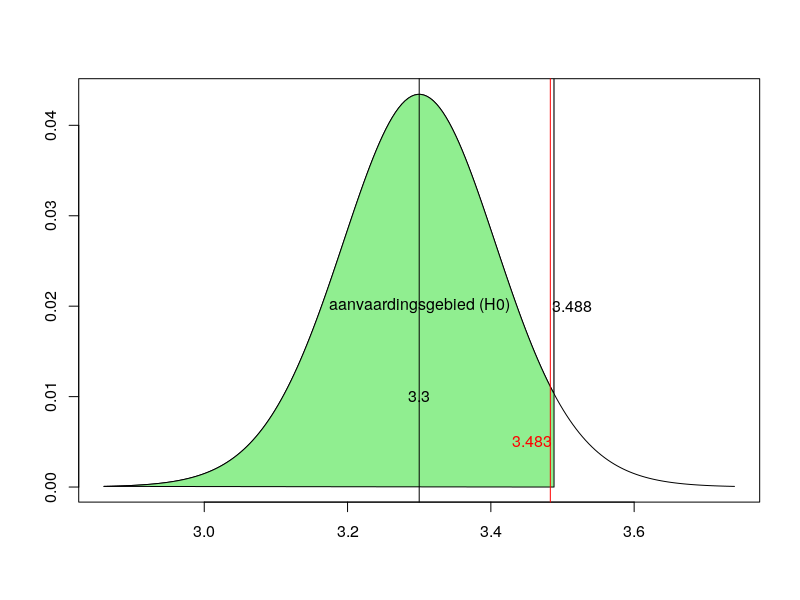
\includegraphics[width=\textwidth]{t-toets-reddingen}
  \caption{R Plot for the case study of Example~\ref{ex:t-test-daily-rescues}}
\end{figure}

\begin{example}
  An outbreak of a Salmonella-induced disease was attributed to vanilla ice cream from a particular factory~\autocite{Lindquist}.
  Scientists measured the level of Salmonella in 9 random samples.
  
  The levels (in MPN/g\footnote{Most Probable Number. See eg.~\url{http://www.microbiologie.info/mpn-methode.html} for more explanation about this method.}) are the following:
  
  \begin{center}
    \begin{tabular}{|l|l|l|l|l|}
      \hline
      0.593 & 0.142 & 0.329 & 0.691 & 0.231 \\ \hline
      0.793 & 0.519 & 0.392 & 0.418 &       \\ \hline
    \end{tabular}
  \end{center}

  Is there a reason to assume that the Salmonella level in the ice is significantly higher than 0.3 MPN/g? 
  We will use the R function \texttt{t.test} to answer this question.
  Read the help page of this function, to get an overview of all possible options.
  
  \begin{enumerate}
    \item Formulate both hypotheses.
    
    $H_0: \mu = 0.3, H_1: \mu > 0,3$
    
    \item Determine significance level $\alpha = 0.05$ and sample size $n = 9$. In R you need to use $1-\alpha = 0.95$.
    
    \item Calculate the probability value. This is a right-tailed test, which can be indicated in R using \texttt{alternative="greater"}. The selected confidence level is the default value of this function and therefore we don't need to add it explicitly.
    
\begin{lstlisting}
x <- c(0.593, 0.142, 0.329, 0.691, 0.231, 0.793, 0.519, 0.392, 0.418)
t.test(x, alternative = "greater", mu = 0.3)
\end{lstlisting}
    
    The result is:
    
\begin{verbatim}
One Sample t-test

data:  x
t = 2.2051, df = 8, p-value = 0.02927
alternative hypothesis: true mean is greater than 0.3
95 percent confidence interval:
0.3245133       Inf
sample estimates:
mean of x 
0.4564444 
\end{verbatim}
    \item Conclusion. The probability value $p = 0.029 < \alpha = 0.05$. Therefore we can reject the null hypothesis; in other words there is a strong indication that the average Salmonella level in the ice is greater than 0.3 MPN/g.
  \end{enumerate}
\textbf{Remark}: \texttt{``confidence interval: 0.3245133 Inf''} has no direct link with the region of acceptance or the critical region.
Is is also unrelated to the value $\mu_{0}=0.3$. 
It only indicates that because $\overline{x}=0.45644$,
we can say with 95\% confidence that the \textit{\'real\'} mean of the population ($\mu$) is between $0.3245133$ and $+\infty$.


See Section~\ref{ssec:confidence-interval-pop-mean-large-sample} (p.~\pageref{ssec:confidence-interval-pop-mean-large-sample}) and Section~\ref{ssec:confidence-interval-pop-mean-small-sample} (p.~\pageref{ssec:confidence-interval-pop-mean-small-sample}) for more information about confidence intervals.
\end{example}


\section{Errors in Hypothesis Tests}

In statistical hypothesis testing, errors can still occur. A type I error occurs when we reject a true null hypothesis $H_{0}$ (also known as a false positive). If we do not reject a false hypothesis $H_{0}$, we make a type II error (or false negative).

When performing a hypothesis test, the significance level $\alpha$ determines when exactly the null hypothesis can be rejected. Suppose we select a significance level of 5\%.
If the null hypothesis is true, the probability of taking a sample in the region of rejection is 5\%. 
In other words, the probability of rejecting a true null hypothesis is 5\%, or in general: the significance level of a test is equal to the probability of making a type I error.

Obviously, we want to minimize the risk of making a type I error.
Unfortunately, this is at the cost of a higher chance of making a type II error, denoted by $\beta$.
The relationship between $\alpha$ and $\beta$ is not trivial and out of scope for this course.

In many cases a type I error is worse than a type II error.
Think of a lawsuit where the null hypothesis states that the person is innocent.
If we test using a confidence level of 5\%, the probability of making a type I error is 5 out of 100.
In other words, there is a confidence of 95\% that the correct decision is made if $H_{0}$ is correct.
Because of this we try to avoid the conclusion that $H_{0}$ is accepted, 
but rather that the sample contains insufficient evidence to reject $H_{0}$ for a given significance level.

\begin{table}
  \centering
  \begin{tabular}{@{}l|cc@{}}
    \toprule
    & \multicolumn{2}{c}{\textbf{Reality}} \\
    \textbf{Decision}             & \textbf{$H_{0}$ True} & \textbf{$H_{1}$ True}     \\
    \midrule
    \textbf{$H_{0}$ not rejected} & Correct                       & Type II error (false negative) \\
    \textbf{$H_{0}$ rejected}     & Type I error (false positive) & Correct            \\
    \bottomrule
  \end{tabular}
  \caption{Conclusions and consequences when thesting a hypothesis; error types.}
  \label{tab:hypfouten}
\end{table}

\section{Exercises}
\label{sec:testing-procedures-exercises}

Source files for these exercises can be found in the Github repo, folder \texttt{exercises/datasets/}.



\begin{exercise}
  \label{ex:binding-recommendation}
  
  It is being said that introducing a ``binding recommendation on continuation of studies'' (refusing enrollment in the next academic year if a student did not complete a certain level of credits) has a positive effect on the study efficiency and success rate. Before the introduction of binding recommendations, the number of completed credits per student per year was 44 with a standard deviation of 6.2. After the introduction, a sample of 72 random students has an average number of completed credits of 46.2.
  
  \begin{enumerate}
    \item Test whether there is evidence that the introduction of binding recommendations has improved the success rate among students. Calculate the critical value for a significance level of $\alpha = 2.5\%$.
    \item Do the same by calculating the $p$-value.
    \item Explain what $\alpha = 2.5 \%$ means.
  \end{enumerate}
\end{exercise}

\begin{exercise}
  \label{ex:price-difference-cars}
  
  One of the motives for choosing a car dealership is the resale value of the previous car, or more specifically the price a dealer wants to pay for the old car when the customer buys a new one. The importer of Ford wants that all dealers implement the same price policy. The importer is of the opinion that the average price difference between the closest Ford dealer and the dealer where the old car was purchased should be at most \euro{300}. It is assumed that, if the difference is larger, potential customers will be more inclined to stay with their previous dealer.
  
  In a random sample, the following price differences are recorded:
  
  \begin{center}
    \begin{tabular}{|l|l|l|l|l|l|l|}
      \hline
      400 & 350 & 400 & 500 & 300 & 350 & 200 \\ \hline
      500 & 200 & 250 & 250 & 500 & 350 & 100 \\ \hline
    \end{tabular}
  \end{center}

  Test whether there is reason to assume that the average price difference in reality is significantly greater than \euro{300}, using a significance level of 5\%.
  
\end{exercise}

\begin{exercise}
  \label{ex:z-test-rlanders}
  Import the dataset \texttt{rlanders-generated.csv}~\footnote{This dataset was generated using \url{https://rlanders.net/dataset-generator/}} in R.
  
  The variable \emph{Money} represents a gross annual salary ($\times 100\$$). We assume this variable has a mean of $\mu = 500$ with standard deviation $\sigma = 98$. If we calculate the sample mean over the total dataset (do it yourself!), it seems to support our assumptions. But what if we looked at men and women separately (variable \emph{Gender})?
  
  Use an appropriate statistical test to verify the statements below, usinge a significance level of $\alpha = 5\%$.
  For each statement, calculate the critical value(s) and the p-value.
  
  \begin{enumerate}
    \item The average gross annual salary of men seems \emph{higher} than the average. Is it also significantly higher?
    \item The average gross annual salary of women seems \emph{lower}. Is it significantly lower?
    \item Calculate the region of acceptance for the average gross annual salary for the sample (men and women combined). In this case we want to verify if the sample mean is significantly different from the expected value, but it can be lower or higher.
  \end{enumerate}
  
\end{exercise}

\section{Solutions to selected exercises}
\label{sec:testing-procedures-solutions}

\paragraph{Exercise~\ref{ex:critical-value-left-tail}:}

\begin{equation}
g = \mu - z \times \frac{\sigma}{\sqrt{n}}
\label{eq:kritiekeRechtseWaarde2}
\end{equation}

because

\[ P(M < g) = P\left(Z < \frac{g - \mu}{\frac{\sigma}{\sqrt{n}}}\right) = 0,05 \]

Thanks the symmetry rule, we know that:
\[ P\left(Z > - \left( \frac{g - \mu}{\frac{\sigma}{\sqrt{n}}} \right) \right) = 0,05 \]

The corresponding z-value is 1.645, and therefore:
\[ z = \frac{-g + \mu}{\frac{\sigma}{\sqrt{n}}} \]
\[ \Leftrightarrow -g = \frac{\sigma}{\sqrt{n}} z - \mu \]
\[ \Leftrightarrow g = -\frac{\sigma}{\sqrt{n}} z + \mu \]

\paragraph{Exercise~\ref{ex:binding-recommendation}}

\begin{enumerate}
  \item $g \approx 45.4 < \overline{x} = 46.2$.
  
  $\overline{x}$ is inside the critical region, so we can reject the null hypothesis. Therefore, we can assume that binding recommendation on continuation of studies does increase the success rate.
  
  \item $P(M > 46.2) \approx 0.0013 < \alpha = 0.025$. The probability value is smaller than the significance level, so we can reject the null hypothesis.
  
  \item  $\alpha$ is the probability of rejecting a true null hypothesis $H_{0}$. In other words, there is a 2.5\% chance that you wrongly conclude that the success rate has increased.
\end{enumerate}

\paragraph{Exercise~\ref{ex:price-difference-cars}}

In this context ($n = 14 < 30$) the $z$-test cannot be used. Instead, we use Student's $t$-test.

\begin{itemize}
  \item $\overline{x} \approx 332.143$
  \item $s \approx 123.424$
  \item $g \approx 358.42$. The sample mean is outside of the critical region, so we cannot reject $H_0$.
  \item $p \approx 0.1738$. $p \nless \alpha$, so we cannot reject $H_0$.
\end{itemize}

Based on this sample there is no reason to assume that the average price difference on the residual value of old cars is significantly greater than the amount recommended by the importer.

\paragraph{Exercise~\ref{ex:z-test-rlanders}}

The mean of the whole sample is $\overline{x} \approx 501.156$

\begin{enumerate}
  \item Only men (right-tailed $Z$-test):
    \begin{itemize}
      \item $\overline{x}_m \approx 507.535$
      \item $g_m \approx 511.456$
      \item $p_m \approx 0.1396$
      \item We \textit{cannot} reject the null hypothesis. The average gross annual salary of men is the sample is not significantly higher than the average.
    \end{itemize}
  \item Only women (left-tailed $Z$-test):
    \begin{itemize}
      \item $\overline{x}_f \approx 472.058$
      \item $g_f \approx 477.646$
      \item $p_f \approx 0.0199$
      \item We \text{can} reject the null hypothesis. The average gross annual salary of women in the sample is significantly lower than the average.
    \end{itemize}
  \item The region of acceptance corresponds to the interval [487.852; 512.148].
\end{enumerate}
 
\chapter{Bivariate Analysis}
\label{ch:bivariate-analysis}
\chapter{Time Series}
\label{ch:time-series}

In previous chapters, we have always analyzed data collected at a specific moment in time and we made statements about that data for that specific moment.

However, within the context of IT, it might be required to monitor data that is constantly changing. For example, think of the load on a processor, the evolution of disk usage on a storage device, the response time of a website, etc.

In this chapter we will examine this type of data and discuss the main analysis methods.

\section{Learning Goals}
\label{sec:time-series-learning-goals}

By the end of this chapter you must be able to:

\begin{itemize}
  \item Explain the following concepts:
  \begin{itemize}
    \item Time series, moving average
  \end{itemize}
  \item For a given time series, i.e. a series of observations from a time series:
  \begin{itemize}
    \item Apply the moving average method;
    \item Based on a plot of observations, estimate what type of exponential smoothing (basic, double, triple/Holt-Winters) is best suited;
    \item Predict future values;
  \end{itemize}
  \item Understand and explain the formulas for the moving average and exponential smoothing, in particular, to estimate the effect of the value of parameters; 
\end{itemize}

  \section{Time Series \& Predictions}

  \begin{definition}[Time Series]
    A \emph{time series} is a sequence of observations of an arbitrary variable in time order.
\end{definition}

Examples:

\begin{itemize}
	\item monthly demand for milk
	\item annual intake of students at HOGENT
	\item daily flow rate of a river
	\item the outside temperature over the course of a day
\end{itemize}

Predicting time series is an important part of research because they often form the basis for decision models. Examples include:

\begin{itemize}
	\item general development of future plans (investments, capacity \dots)
	\item budget planning to avoid shortcomings (operating budget, marketing budget \dots)
	\item competitive delivery times of a company
	\item support for financial objectives
	\item avoid uncertainty
	\item the possibility to quantitatively model developments in road safety
\end{itemize}


Modeling time series is a statistical problem: we assume that the observations vary according to a certain probability density function as a function of time. We often assume that the observations in a time series are correlated and therefore are not obtained from a random sample.

Different model types are used to analyze time series. These models have in common that in principle they can not only describe the development in an observed time series, but they can also be used to

\begin{itemize}
	\item find explanations for this development and
	\item to predict the future values of the time series.
\end{itemize}

However, their suitability for achieving these objectives varies widely. In this chapter we limit ourselves to using time series with a history to determine time dependent models. An example of a time series is the age of the successive kings of England starting from William The Conqueror \autocite{Hipel1994}.

\begin{lstlisting}
kings <- scan(file = 'syllabus/data/time-series/kings.data', skip = 3)
kingstimeseries <- ts(kings)
plot.ts(kingstimeseries, ylab='age', xlab="time")
grid(lty=2,lwd=1,col='black')
\end{lstlisting}

\begin{figure}
	\centering
	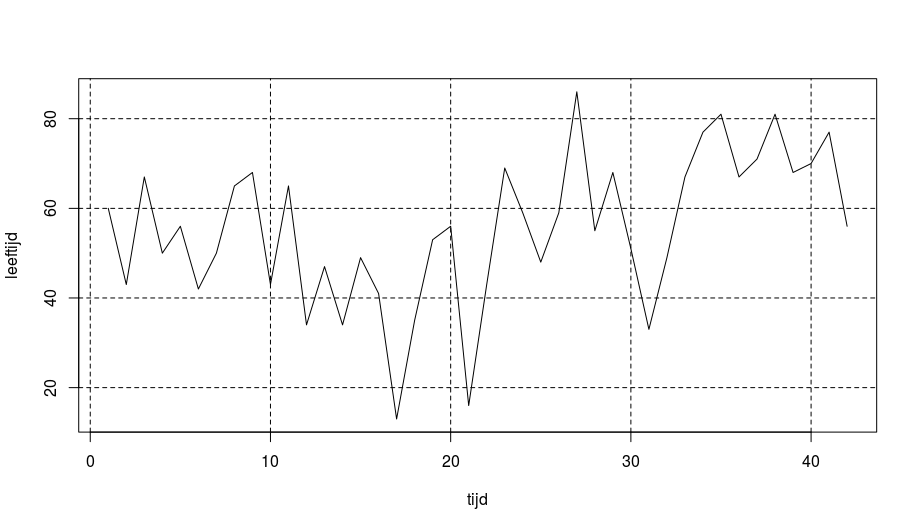
\includegraphics[width=\textwidth]{time-series/time-series-kings.png}
	\caption{The time series representing the ages of the kings.}
	\label{fig:time-series-11}
\end{figure}

\section{Time series models}

\subsection{Mathematical model}

Our goal is to create a model that explains the observed data and that allows to predict future observations as accurately as possible. The simplest model you can think of is a model where a constant $b$ is used with variations around $b$ determined by a random variable $\epsilon_{t}$ as in Equation~\ref{eq:constant}.

\begin{equation}
	X_{t} = b + \epsilon_{t}
\label{eq:constant}
\end{equation}

\begin{description}
  \item [$X_{t}$] represents a \emph{variable} that is unknown at time $t$.
  \item [$x_{t}$] represents an \emph{observation} at time $t$ (and is known). 
  \item [$\epsilon_{t}$] is called the \emph{noise} and is considered to have a mean of $0$ with variance $\sigma^{2}$ and has a normal distrbution ($\epsilon_{t} \sim Nor(0, \sigma)$). 
\end{description}

We could also assume that there is a linear relationship:

\begin{equation}
  X_{t} = b_{0} + b_{1} \times t + \epsilon_{t}
  \label{eq:linear8}
\end{equation}

The equation in \ref{eq:constant} and \ref{eq:linear8} are special cases of the polynomial case:

\begin{equation}
	X_{t} = b_{0} + b_{1} t + b_{2} t^{2} + \dots + b_{n} t^{n} + \epsilon_{t} 
\label{eq:polynomial}
\end{equation}

\begin{exercise}
	What could the following time series represent?
	\begin{equation}
		X_{t} = b_{0} + b_{1} \sin\left(\frac{2\pi t}{4}\right) + b_{1} \cos\left(\frac{2\pi t}{4}\right) + \epsilon_{t}
	\label{eq:seasonal}
\end{equation}
\end{exercise}

Answer: This is a cyclic time series with period $= 4$. This could for example be used with a time series for seasons.

\begin{lstlisting}
f <- function(a, b,t){
  return(a + b * sin((2 * pi*4)/4) + b * cos((2 * pi*4)/4) + rnorm(1))
}
t <- seq(from = 1, to = 100, by = 1)
X <- lapply(t,f,a=5,b=5)
plot(x = t, y=X, type = 'l')
\end{lstlisting}

\subsubsection{General}

In each considered model, the time series is a function of time and parameters of the model. In general, we can say that:

\begin{equation}
	X_{t} = f(b_{0}, b_{1}, b_{2}, \dots , b_{t}, t) + \epsilon_{t}
\label{eq:general}
\end{equation}

We then accept the following statements:

\begin{itemize}
	\item The model assumes two components of variability: the mean of the predictions changes with time and the variations to this mean vary randomly.
	\item The residuals of the model ($X_{t} - x_{t}$) are homoscedastic: this means that they have a constant variance in time.
\end{itemize}

Once the model is chosen, all that remains is the problem of estimating the parameters for Equation~\ref{eq:general}. This will be discussed in the following sections.

\section{Estimating the parameters}

Once a model is selected, it is up to the researcher to estimate the parameters, i.e. find parameters that ensure that the model approximates the observed values as closely as possible. We usually assume that all values are equivalent, but this is not the case with time series. Since our independent parameter is time, we need to obtain methods that make more recent data more important than old data or vice versa.

In what follows we describe the time series with estimated values for the parameters. We indicate estimators by using a hat on the parameters:

\[ \widehat{b}_{1}, \widehat{b}_{2} \dots \widehat{b}_{n} \]

\subsection{Moving average}

\begin{table}
  \centering
  \begin{tabular}{|l|l|l|l|l|l|l|l|l|l|}
    \hline
    4 & 16 & 12 & 25 & 13 & 12 & 4 & 8  & 9 & 14 \\ \hline
    3 & 14 & 14 & 20 & 7  & 9  & 6 & 11 & 3 & 11 \\ \hline
    8 & 7  & 2  & 8  & 8  & 10 & 7 & 16 & 9 & 4  \\ \hline
  \end{tabular}
  \caption{Time series data example, visualized in Figure~\ref{fig:time-series-21}.}
  \label{tab:data-time-series-21}
\end{table}

Suppose a researcher has the data of Table~\ref{tab:data-time-series-21} up to the twentieth point available (known data). The researcher does not know the subsequent data points and has to predict them. A first model that could be used is the constant model from Equation~\ref{eq:constant}.

According to this model, the data points are considered as random values from a population with a mean $b$. The best estimator for $b$ is the mean of these twenty data points.

\begin{lstlisting}
data <- c(4 , 16 , 12 , 25 , 13 , 12 , 4 , 8  , 9 , 14, 
+           3 , 14 , 14 , 20 , 7  , 9  , 6 , 11 , 3 , 11, 
+           8 , 7  , 2  , 8  , 8  , 10 , 7 , 16 , 9 , 4 )
mean(data[1:20])
\end{lstlisting}

\[ \widehat{b} = \frac{1}{20} \sum_{1}^{20} x_{t}= 10.75 \]

This is the best estimator based on the 20 data points. However, note that $x_{1} =  4$ has as much \textit{value} as  $x_{20} = 11$, or in other words: the coefficient of $x_{1}$ is the same as the coefficient of $ x_ {20} $, which is $\frac{1}{20}$.

If we use this as an estimator, Figure~\ref{fig:time-series-21} illustrates that this is not a good idea.

\begin{lstlisting}
AV20 <- matrix(10.75,30,1)
plot.ts(data, col="blue", type='b', xlab='time', ylab='Data')
lines(AV20,col='red', type='l')
legend(x= 'topright',legend = c("Data","Mean 10.75"), lty = c(1,1), lwd = c(2.5,2.5), col=c('blue','red'))
\end{lstlisting}

\begin{figure}
	\centering
		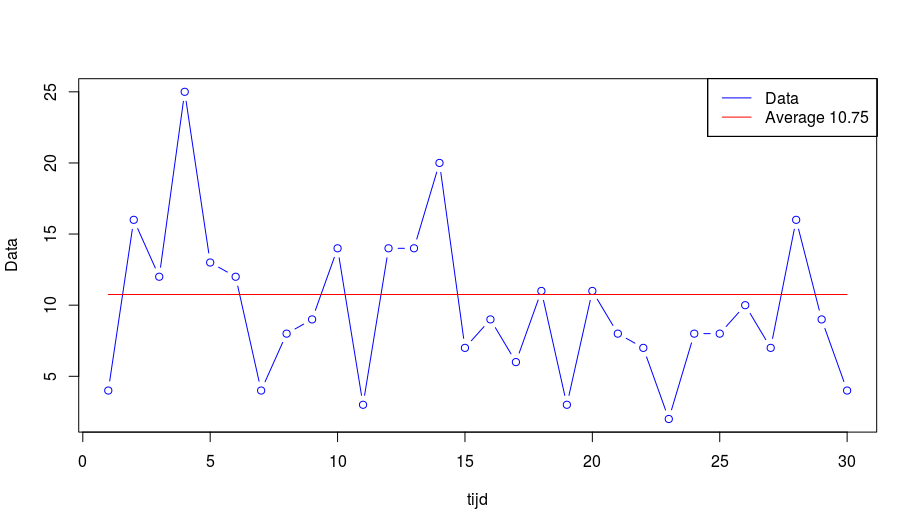
\includegraphics[width=1.00\textwidth]{time-series/time-series-20.png}
	\caption{Time series with constant mean $10.75$}
	\label{fig:time-series-21}
\end{figure}

If we assume that the data changes over time, it is better to have old data count less than more recent ones. One possibility is to use only recent data, for example the 10 or 5 last data points (cfr. Figure \ref{fig:time-series-31}).

\[ \widehat{b} = \frac{1}{10} \sum_{10}^{20} x_{t} = 10.18 \] and
\[ \widehat{b} = \frac{1}{5} \sum_{15}^{20} x_{t} = 7.83 \]

\begin{lstlisting}
sma10 <- SMA(x =data,n=10)
sma5 <- SMA(x=data,n=5)
plot.ts(x = data, col = 'blue',type = 'l')
lines(sma10, col='red', type = 'b')
lines(sma5, col='purple', type = 'b')
\end{lstlisting}

\begin{figure}
  \centering
    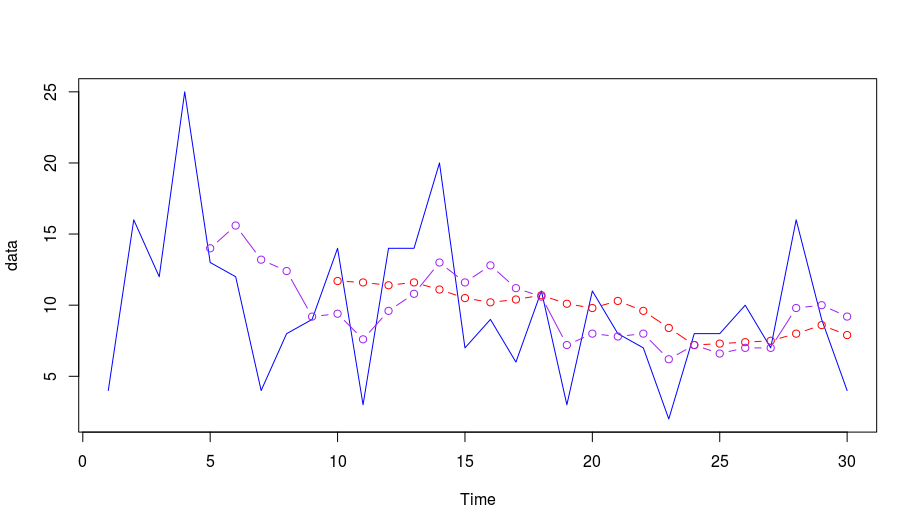
\includegraphics[width=1.00\textwidth]{time-series/time-series-sma.png}
    \caption{Time series with moving average $m = 10$ and $m=5$}. 
  \label{fig:time-series-31}
\end{figure}

These are called \textit{moving averages}\index{moving average}.

Which estimator is now best? We cannot answer this yet.

\begin{itemize}
  \item The estimator using all data points is best if the time series follows the model completely.
  \item The estimator with the more recent data points is best if the time series changes over time.
\end{itemize}

\begin{definition}[moving average]
  In general the \emph{moving average} is the average (mean) of the last $m$ observations.
  \begin{equation}
    \widehat{b} = \sum_{i=k}^{t} \frac{x_{i}}{m}
  \label{eq:movingAverage}
  \end{equation}
  with $k = t-m+1$. $m$ is the time range and is the parameter of the method.
\end{definition}

\subsection{Measuring the accuracy of predictions}

%\begin{table}
%  \centering
%\begin{tabular}{|lllllllllll|}
%
%\end{tabular}
%\caption{Voorspellingsfout voor een moving average $m = 10$}
%\label{tab:error}
%\end{table}

One method for measuring the prediction is calculating the mean absolute deviation ($MAD$): the mean of the absolute differences between the predicted and actual values of the time series.

\begin{definition}[$MAD$]
  \begin{equation}
    MAD = \frac{1}{n} \sum_{1}^{n} \left| e_{i} \right|  
  \label{eq:MAD}
  \end{equation}
\end{definition}

You can also percentage this to calculate the mean absolute percentage error ($MAPE$), also known as mean absolute percentage deviation ($MAPD$).

\begin{definition}[$MAPE$]
  \begin{equation}
    MAPE = \frac{1}{n} \sum_{1}^{n} \left| \frac{e_{i}}{X_i} \right|  
  \label{eq:MAD2}
  \end{equation}
\end{definition}

It is also possible to calculate the variance of the errors:

\begin{definition}[$VAR$]
\begin{equation}
	s^{2}_{e} = \frac{1}{m} \sum_{1}^{n} (e_{i} - \overline{e})^{2}
\label{eq:varError}
\end{equation}
\end{definition}

% TODO: moet de noemer hierboven niet n - 1 zijn??

A last insteresting parameter is the root-mean-square error ($RMSE$) or root-mean-square deviation ($RMSD$), which is the square root of the mean of the squared difference between the predicted and the actual values of the time series.

\begin{definition}[$RMSE$]
  \begin{equation}
    RMSE_{e} = \sqrt{\frac{1}{m} \sum_{1}^{n} (e_{i})^{2}}
  \label{eq:varError2}
  \end{equation}
\end{definition}

\section{Exponential smoothing}

When calculating a moving average, all previous observations have equal weight. With exponential smoothing, however, smaller weights are assigned to older observations. In other words, more recent observations gain relatively more weight than older observations.

In the case of the simple moving average, all weights are the same, namely $\frac{1}{m}$.

\subsection{Basic exponential smoothing}

Exponential smoothing is a weighted arithmetic mean that assigns positive weights to the current and past values of a time series. A single weight, $0\leq \alpha \leq1$ or the smoothing constant is selected for this. For a given time $t$, the basic exponential smoothing can be found using Equation \ref{eq:singleExpSmooting}.

\begin{definition}[Exponential Smoothing]
  \begin{equation}
    X_{t} = \alpha x_{t} + (1-\alpha)X_{t-1}, 0 \leq \alpha \leq 1, t \geq 3
  \label{eq:singleExpSmooting}
  \end{equation}
\end{definition}

In other words, $X_{t}$ is a weighted arithmetic mean of the current observation $x_t$ and the previous exponential smoothing $X_{t-1}$.

\subsection{Initial value}
Determining $X_{2}$ is an important parameter. You could choose to:
\begin{enumerate}
  \item assume that $X_{2} = x_{1}$
  \item make $X_{2}$ equal to a specific objective
  \item take the mean of the first $x$ observations
  \item \dots
\end{enumerate}

Why is this called an exponential method? If we were to substitute we find e.g. for $X_{t-1}$:

\[ X_{t} = \alpha x_{t} + (1-\alpha)\left[\alpha x_{t-1} + (1-\alpha)X_{t-2}\right] \] 
\[ X_{t} = \alpha x_{t} + \alpha (1-\alpha)x_{t-1} + (1-\alpha)^{2} X_{t-2} \]
or in general:
\[ X_{t} = \alpha \sum_{i=0}^{t-2}(1-\alpha)^{i-1}x_{t-i} + (1-\alpha)^{t-2} X_{2}, t \geq 2 \]

You will notice that older components have an exponentially smaller weight.

\subsubsection{Value of $\alpha$}
The speed at which the old observations are ``forgotten'' depends on the value of $\alpha$. For a value of $\alpha$ close to 1, old observations are quickly forgotten , whereas for  $\alpha$ close to 0, this goes less fast (as illustrated in Table \ref{tab:alpha}). Often a value between $0.10$ and $0.30$ is used.

\begin{table}
  \centering
  \begin{tabular}{l|llll}
  $\alpha$ & $(1-\alpha)$ & $(1-\alpha)^{2}$ & $(1-\alpha)^{3}$ & $(1-\alpha)^{4}$ \\ \hline
  0.9   & 0.1       & 0.01             & 0.001                      & 0.0001           \\
  0.5   & 0.5       & 0.25             & 0.125                      & 0.062            \\
  0.1   & 0.9       & 0.81             & 0.729                      & 0.6561           \\
  \end{tabular}
  \caption{Values for $\alpha$ and $(1-\alpha)^{n}$}
  \label{tab:alpha}
  \end{table}

  For example, the file \texttt{precip.data} contains the total annual rainfall in inches for London, between 1813 and 1912. Let's analyse this in R.
  
\begin{lstlisting}
rain <- scan("cursus/data/tijdreeksen/precip.data",skip=1)
rainseries <- ts(rain,start=c(1813))
plot.ts(rainseries)
plot(rainseriesforecasts)
\end{lstlisting} 

%TODO figuur maken voor verschillende alpha's

\subsubsection{Prediction with exponential smoothing}

Suppose the goal is to predict the next value $X_{t+1}$, this is equal to calculating the the smoothing value at time $t$.

\begin{equation}
	X_{t+1} = EMA_t = X_t
	\label{eq:EMA}
\end{equation}

With $X_t$ the last predicted value.

This can be easily done in R. The outcome is a \emph{prediction interval}, an interval for which we expect the predicted value to be included with a certain probability. By default, an 80\% and a 95\% interval are returned.

\begin{lstlisting} 
library('forecast')
rainseriesforecasts2 <- forecast.HoltWinters(rainseriesforecasts, h=8)
plot.forecast(rainseriesforecasts2)
\end{lstlisting} 

We should see correlations between the prediction errors for subsequent predictions. In other words, if there is a correlation between forecast errors for subsequent predictions, it is more likely that the simple exponential smoothing can be corrected by using a different prediction technique.

To find out if this is the case, we can obtain a correlogram of the in-sample prediction errors.

We remembers from Chapter~\ref{ch:bivariate-analysis} that the covariance or correlation describe the relationship between two variables. The autocovariance and autocorrelation measure the linear relationship between time-shifted values for a time series.

\begin{definition}[Autocovariance]
  We define the autocovariance for a lag $k$ as $c_k$.
	\[ c_k = \sum_{t=k+1}^{T} (y_t - \overline{y})(y_{t-k} - \overline{y}) \]
\end{definition}

\begin{definition}[Autocorrelation]
  We define the autocorrelation for a lag $k$ as $r_k$.
	\[ r_k = \frac{c_k}{c_0} \]
\end{definition}

A correlogram is a plot of the autocorrelations. You can plot this in R by using the function \texttt{acf()}. This also calculates the prediction errors. To determine the maximum lag (delay) we want to view, we use the parameter \texttt{lag.max}.

For example, to calculate a correlogram of the forecast errors for the London rainfall data for a lag between 1 and 20, we use:

\begin{lstlisting}
acf(rainseriesforecasts2$residuals, lag.max=20, na.action = na.pass)
\end{lstlisting}

To test whether there is significant evidence for significant correlations at a lag 1-20, we can apply a Ljung-Box test. This can be done in R using the function \texttt{Box.test()}. The maximal lag (or delay) we want to investiage, is specified using the parameter \texttt{Lag}.

A full explanation of this test is out of scope for this course, but the test assumes the hypotheses $H_0$ and $H_1$ as formulated below. The tes statistics can then be interpreted in a similar way as all other  hypothesis tests described in the previous chapters.

\begin{itemize}
  \item $H_0$ The data are independently distributed (in other words, the correlations in the population from which the sample is taken are 0, and therefore  any observed correlations in the data result from randomness of the sampling process).
  \item $H_1$ The data are not independently distributed, they exhibit linear (serial) correlation.
\end{itemize}

For example, to test that there are no zero autocorrelations for a lag 1-20, for the in-sample predictions errors for London rainfall data, we type:

% TODO: correcte Nl term voor in-sample error?

\begin{lstlisting}
Box.test(rainseriesforecasts2$residuals, lag=20, type="Ljung-Box")
Box-Ljung test
data:  rainseriesforecasts2$residuals
X-squared = 17.4008, df = 20, p-value = 0.6268
\end{lstlisting}

Finally, we should also look at the distribution of the errors of the forecast. As mentioned above, we assume that the errors are normally distributed with an average $\mu = 0$ and a constant standard deviation. To verify this assumption, we can plot a histogram of the forecast errors, with an overlapping normal curve with mean zero and the same standard deviation as the distribution of the prediction errors. For this, we can define a function in R \texttt{plotForecastErrors()}. It is also recommended to use the methods described in Section~\ref{ssec:testing-for-normality}.

% TODO: zin onvolledig

\begin{lstlisting}
plotForecastErrors <- function(forecasterrors)
{
# make a histogram of the forecast errors:
mybinsize <- IQR(forecasterrors)/4
mysd   <- sd(forecasterrors)
mymin  <- min(forecasterrors) - mysd*5
mymax  <- max(forecasterrors) + mysd*3
# generate normally distributed data with mean 0 and standard deviation mysd
mynorm <- rnorm(10000, mean=0, sd=mysd)
mymin2 <- min(mynorm)
mymax2 <- max(mynorm)
if (mymin2 < mymin) { mymin <- mymin2 }
if (mymax2 > mymax) { mymax <- mymax2 }
# make a red histogram of the forecast errors, with the normally distributed data overlaid:
mybins <- seq(mymin, mymax, mybinsize)
hist(forecasterrors, col="red", freq=FALSE, breaks=mybins)
# freq=FALSE ensures the area under the histogram = 1
# generate normally distributed data with mean 0 and standard deviation mysd
myhist <- hist(mynorm, plot=FALSE, breaks=mybins)
# plot the normal curve as a blue line on top of the histogram of forecast errors:
points(myhist$mids, myhist$density, type="l", col="blue", lwd=2)
}
\end{lstlisting}

\subsection{Double exponential smoothing}

Basic exponential smoothing is used when no trend is visible. When there is a visible trend (increasing or decreasing) errors may occur. For example, take a look at the data in Table~\ref{tab:trend} and Figure~\ref{fig:time-series-61}.

\begin{table}
  \centering
    \begin{tabular}{|ll|}
    \hline
    Data & Basic exponential smoothing \\
    6.4  & ~                      \\
    5.6  & 6.4                    \\
    7.8  & 6.2                    \\
    8.8  & 6.7                    \\
    11.0 & 7.3                    \\
    11.6 & 8.4                    \\
    16.7 & 9.4                    \\
    15.3 & 11.6                   \\
    21.6 & 12.7                   \\
    22.4 & 15.4                   \\ \hline
    \end{tabular}
    \caption{Basic exponential smoothing with $\alpha = 0.3$}
    \label{tab:trend}
\end{table}
  
\begin{figure}
  \centering
  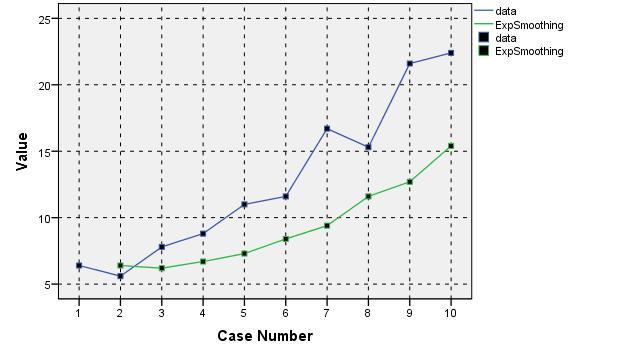
\includegraphics[width=1.00\textwidth]{time-series/time-series-61.jpg}
  \caption{Exponential smoothing for a trend}
  \label{fig:time-series-61}
\end{figure}

Therefore, we add an extra constant to bridge this gap:

\begin{definition}[Holt forcasting or double exponential smoothing]
\begin{eqnarray}
  X_{t} = \alpha x_{t} + (1-\alpha)(X_{t-1} + b_{t-1}) & 0 \leq \alpha \leq 1 \\
  b_{t} = \beta(X_{t}-X_{t-1}) + (1-\beta)b_{t-1} & 0 \leq \beta \leq 1 
\label{eq:doubleSmoothing}
\end{eqnarray}
\end{definition}

\subsection{Initial value}

As with basic exponential smoothing, there are different methods for selecting the initial values of $X_{t}$ and $b_{t}$:

\begin{itemize}
	\item $X_{1} = x_{1}$
	\item $b_{1} = x_{2} - x_{1}$
	\item $b_{1} = \frac{1}{3}\left[ (x_{2} - x_{1}) + (x_{1} - x_{2}) + (x_{4} - x_{3}) \right]$
	\item $b_{1} = \frac{x_{n} - x_{1}}{n-1}$
\end{itemize}

\subsubsection{Prediction}

Making a prediction when using double exponential smoothing is slightly different ($F_{t+1}$ is used as prediction for time $T+1$):

\[ F_{t+1} = X_{t} + b_{t} \]
or
\[ F_{t+m} = X_{t} + m b_{t} \]

If we now draw a plot with basic exponential smoothing ($\alpha = 0.977$) and double exponential smoothing ($\alpha = 0.3623, \beta = 1.0, X_{1} = x_{1} = 6.4$ and $b_{1} = \frac{1}{3}\left[ (x_{2} - x_{1}) + (x_{1} - x_{2}) + (x_{4} - x_{3}) \right] = 0.8$) we obtain the values of Table \ref{tab:doubleSingle} and Figure \ref{fig:time-series-71}:

\begin{table}
  \centering
  \begin{tabular}{|llll|}
    \hline
    Data & Basic exponential smoothing $X_{t}$ & Double exponential smoothing $X_{t}$ & $F_{t}$ \\
    6.4  & ~                      & 6.4              & ~                             \\
    5.6  & 6.4                    & 6.6              & 7.2                           \\
    7.8  & 5.6                    & 7.2              & 6.8                           \\
    8.8  & 6.7                    & 8.1              & 7.8                           \\
    11.0 & 8.8                    & 9.8              & 9.1                           \\
    11.6 & 10.9                   & 11.5             & 11.4                          \\
    16.7 & 11.6                   & 14.5             & 13.2                          \\
    15.3 & 16.6                   & 16.7             & 17.4                          \\
    21.6 & 15.3                   & 19.9             & 18.9                          \\
    22.4 & 21.5                   & 22.8             & 23.1                          \\ \hline
  \end{tabular}
  \caption{Table with basic and double exponential smoothing}
  \label{tab:doubleSingle}
\end{table}

\begin{figure}
	\centering
		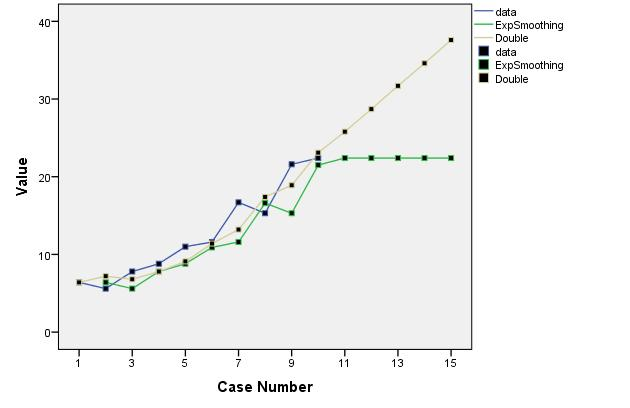
\includegraphics[width=1.00\textwidth]{time-series/time-series-71.jpg}
	\caption{Basic and double exponential smoothing}
	\label{fig:time-series-71}
\end{figure}

The procedure to solve this in R is similar to the procedure for basic exponential smoothing, except that the parameter $\beta$ should not be set to NULL. Creating the correlogram, applying the Ljung–Box test and testing the normality of the errors is done in a similar way.

\subsection{Triple exponential smoothing}

In many time series you will see that certain patterns recur. For example, take the daily turnover of a bakery: the turnover will be different every day, but if you look at it over a long period of time, you will probably see a similar pattern every week (with a top turnover on Sunday, for example).

This type of time series can be approximated by using the Holt-Winter method, or triple exponential smoothing.

\begin{eqnarray}
  X_{t} = \alpha \frac{x_{t}}{c_{t-L}} + (1-\alpha) (X_{t-1} + b_{t-1}) & \textnormal{Smoothing}\\
  b_{t} = \beta (X_{t} - X_{t-1}) + (1-\beta)b_{t-1} & \textnormal{Trend smoothing} \\
  c_{t} = \gamma \frac{x_{t}}{X_{t}} + (1-\gamma)c_{t-L} & \textnormal{Seasonal smoothing} \\
  F_{t+m} = (X_{t} + mb_{t})c_{t-L+m \mod L}  & \textnormal{Prediction}
  \label{eq:HoltWinters}
\end{eqnarray}
 with
\begin{itemize}
	\item $x_{t}$ the observation at time $t$
	\item $X_{t}$ the smoothed observation at time $t$
	\item $b_{t}$ the trend factor at time $t$
	\item $c_{t}$ the seasonal index at time $t$
	\item $F_{t}$ the prediction at time $t$
	\item $L$ the period (e.g. of the seasons)
\end{itemize}

$\alpha, \beta en \gamma$ are constants that need to be estimated.
The procedure to solve this in R is similar to the procedure for basic exponential smoothing. Creating the correlogram, applying the Ljung–Box test and testing the normality of the errors is done in a similar way.

\section{Exercises}
\label{sec:time-series-exercises}

\begin{exercise}
  The file \emph{Budget.csv} contains the turnover, advertising budget and GNP (Dutch: BNP) of a medium sized compay per quarter between 1981 and 2005. Add another column yourself that contains an ascending number for each quarter.
  
  \begin{enumerate}
    \item Calculate the basic (or simple) moving average over periods 4 and 12 of this data. Use the SMA method for this. Plot a line graph for $X$, $SMA(4)$ and $SMA(12)$.
    \item Which previously covered technique (from the section on descriptive statistics) is also suitable for making predictions about the values of $X$? Do so using the appropriate function and plot the results in the graph.
    \item Use the \emph{forecast} method to make predictions for the next 10 periods using each of the previous methods (moving average 4, 10 and regression). Also plot the results on the graph.
    \item Is the use of one of these techniques interesting to make predictions for this data?
    \item Create a time series of the data using the method \emph{ts}. Use the \emph{decompose} method to divide the time series and get an idea of the trend and the seasonal fluctuation.
    \item Calculate the exponential moving average (\emph{EMA}) using the method \emph{HoltWinters}. Make another prediction for 20 periods using the \emph{forecast} method. For the initial values, use $s_1 = x_1$ and the value generated by R for $\alpha$. Plot the result in a new graph, together with $X$.
    \item Do the same for $\alpha=0.1$.
    \item What do the predictions look like?
    \item Do the same using \emph{double} exponential smoothing. For the initial values, use $s_1 = x_1$ and $b_1 = \frac{x_n - x_1}{n - 1}$, $\alpha =  0.05$ and $\beta = 0.2$. Plot the result on the graph.
    \item Use double exponential smoothing to calculate predictions for 20 periods. Plot the values on the graph. Is this technique better or worse than the previous one for this dataset?
    \item Experiment with the value $\alpha$ and $\beta$ and look at the result, for both basic and double exponential smoothing.
    \item Use the \emph{HoltWinters} method without trend. In other words, use $\beta=0$. For the initial values, use $\alpha =  0.05$ and $\gamma = 0.9$. Plot the result on the graph.
    \item Again, calculate predictions for 20 periods. Plot the values on the graph. Is this technique better or worse than the previous one for this dataset?
    \item Experiment with the values of $\alpha$, $\beta$ and $\gamma$ and look at the result.
    \item Use the \emph{HoltWinters} method with the values generated by R, but again without using a trend ($\beta=0$). Plot the result on the graph.
    \item Again, calculate predictions for 20 periods but this time by using the function \emph{predict}. Plot the values on the graph. Is this technique better or worse than the previous one for this dataset?
  \end{enumerate}	
  \end{exercise}
  
  \begin{exercise}
  The file \emph{Passagiers2.csv} contains the number of passengers on an airline between January 1949 and December 1960.
  \begin{enumerate}
    \item Calculate the basic (or simple) moving average over periods 4 and 12 of this data. Use the \emph{MA} method for this. Plot a line graph for $X$, $MA(4)$ and $MA(12)$.
    \item Which previously covered technique (from the section on descriptive statistics) is also suitable for making predictions about the values of $X$? Do so using the appropriate function and plot the results in the graph.
    \item Use the \emph{forecast} method to make predictions for the next 10 periods using each of the previous methods (moving average 4, 12 and regression). Also plot the results on the graph. What is your conclusion?
    \item Is the use of one of these techniques interesting for making predictions for this data?
    \item Use the method \emph{decompose} to subdivide the time series and get an idea of the trend and the seasonal fluctuation.
    \item Calculate the exponential moving average (\emph{EMA}) using the \emph{ses} method with $\alpha=0.2$. Make another prediction using the \emph{forecast} method for 20 periods. Plot the result in a new graph, together with $X$.
    \item Do the same for $\alpha=0.6$ and $\alpha=0.89$.
    \item What to the predictions look like now?
    \item Do the same using \emph{double} exponential smoothing. Use the \emph{holt} method for this, with $\alpha =  0.8$ and $\beta = 0.2$. Plot the result on the graph.
    \item Use double exponential smoothing to calculate predictions for 20 periods. Plot the values on the graph. Is this technique better or worse than the previous one for this dataset?
    \item Add the option $exponential=TRUE$ to the method. Plot the result. What is the difference?
    \item Use the \emph{hw} method with the values generated by R. Plot the result on the graph.
    \item Again, calculate a few predictions using the method \emph{predict}. Plot the values on the graph. Is this technique better or worse than the previous one for this dataset?
    \item Experiment with the values for $\alpha$, $\beta$ and $\gamma$ and look at the result.
  \end{enumerate}
  
  \end{exercise}


\begin{appendices}
    %\include{logistic}
    
    \chapter{Notation}
\label{app:notation}
    
    \clearpage
    \addcontentsline{toc}{chapter}{\textcolor{maincolor}{\IfLanguageName{dutch}{Bibliografie}{Bibliography}}}
    \printbibliography
    
    \clearpage
    \addcontentsline{toc}{chapter}{\textcolor{maincolor}{Index}}
    \printindex
    
\end{appendices}
\end{document}
